\documentclass[twoside]{book}

% Packages required by doxygen
\usepackage{fixltx2e}
\usepackage{calc}
\usepackage{doxygen}
\usepackage[export]{adjustbox} % also loads graphicx
\usepackage{graphicx}
\usepackage[utf8]{inputenc}
\usepackage{makeidx}
\usepackage{multicol}
\usepackage{multirow}
\PassOptionsToPackage{warn}{textcomp}
\usepackage{textcomp}
\usepackage[nointegrals]{wasysym}
\usepackage[table]{xcolor}

% NLS support packages
\usepackage[T2A]{fontenc}
\usepackage[russian]{babel}

% Font selection
\usepackage[T1]{fontenc}
\usepackage[scaled=.90]{helvet}
\usepackage{courier}
\usepackage{amssymb}
\usepackage{sectsty}
\renewcommand{\familydefault}{\sfdefault}
\allsectionsfont{%
  \fontseries{bc}\selectfont%
  \color{darkgray}%
}
\renewcommand{\DoxyLabelFont}{%
  \fontseries{bc}\selectfont%
  \color{darkgray}%
}
\newcommand{\+}{\discretionary{\mbox{\scriptsize$\hookleftarrow$}}{}{}}

% Page & text layout
\usepackage{geometry}
\geometry{%
  a4paper,%
  top=2.5cm,%
  bottom=2.5cm,%
  left=2.5cm,%
  right=2.5cm%
}
\tolerance=750
\hfuzz=15pt
\hbadness=750
\setlength{\emergencystretch}{15pt}
\setlength{\parindent}{0cm}
\setlength{\parskip}{0.2cm}
\makeatletter
\renewcommand{\paragraph}{%
  \@startsection{paragraph}{4}{0ex}{-1.0ex}{1.0ex}{%
    \normalfont\normalsize\bfseries\SS@parafont%
  }%
}
\renewcommand{\subparagraph}{%
  \@startsection{subparagraph}{5}{0ex}{-1.0ex}{1.0ex}{%
    \normalfont\normalsize\bfseries\SS@subparafont%
  }%
}
\makeatother

% Headers & footers
\usepackage{fancyhdr}
\pagestyle{fancyplain}
\fancyhead[LE]{\fancyplain{}{\bfseries\thepage}}
\fancyhead[CE]{\fancyplain{}{}}
\fancyhead[RE]{\fancyplain{}{\bfseries\leftmark}}
\fancyhead[LO]{\fancyplain{}{\bfseries\rightmark}}
\fancyhead[CO]{\fancyplain{}{}}
\fancyhead[RO]{\fancyplain{}{\bfseries\thepage}}
\fancyfoot[LE]{\fancyplain{}{}}
\fancyfoot[CE]{\fancyplain{}{}}
\fancyfoot[RE]{\fancyplain{}{\bfseries\scriptsize Документация по Сетевой сервис. Последние изменения\+: Вт 8 Дек 2015 22\+:32\+:12. Создано системой Doxygen }}
\fancyfoot[LO]{\fancyplain{}{\bfseries\scriptsize Документация по Сетевой сервис. Последние изменения\+: Вт 8 Дек 2015 22\+:32\+:12. Создано системой Doxygen }}
\fancyfoot[CO]{\fancyplain{}{}}
\fancyfoot[RO]{\fancyplain{}{}}
\renewcommand{\footrulewidth}{0.4pt}
\renewcommand{\chaptermark}[1]{%
  \markboth{#1}{}%
}
\renewcommand{\sectionmark}[1]{%
  \markright{\thesection\ #1}%
}

% Indices & bibliography
\usepackage{natbib}
\usepackage[titles]{tocloft}
\setcounter{tocdepth}{3}
\setcounter{secnumdepth}{5}
\makeindex

% Hyperlinks (required, but should be loaded last)
\usepackage{ifpdf}
\ifpdf
  \usepackage[pdftex,pagebackref=true]{hyperref}
\else
  \usepackage[ps2pdf,pagebackref=true]{hyperref}
\fi
\hypersetup{%
  colorlinks=true,%
  linkcolor=blue,%
  citecolor=blue,%
  unicode%
}

% Custom commands
\newcommand{\clearemptydoublepage}{%
  \newpage{\pagestyle{empty}\cleardoublepage}%
}


%===== C O N T E N T S =====

\begin{document}

% Titlepage & ToC
\hypersetup{pageanchor=false,
             bookmarks=true,
             bookmarksnumbered=true,
             pdfencoding=unicode
            }
\pagenumbering{roman}
\begin{titlepage}
\vspace*{7cm}
\begin{center}%
{\Large Сетевой сервис }\\
\vspace*{1cm}
{\large Создано системой Doxygen 1.8.9.1}\\
\vspace*{0.5cm}
{\small Вт 8 Дек 2015 22:32:12}\\
\end{center}
\end{titlepage}
\clearemptydoublepage
\tableofcontents
\clearemptydoublepage
\pagenumbering{arabic}
\hypersetup{pageanchor=true}

%--- Begin generated contents ---
\chapter{Алфавитный указатель пространств имен}
\section{Пространства имен}
Полный список пространств имен.\begin{DoxyCompactList}
\item\contentsline{section}{\hyperlink{namespace_network_service}{Network\+Service} }{\pageref{namespace_network_service}}{}
\end{DoxyCompactList}

\chapter{Иерархический список классов}
\section{Иерархия классов}
Иерархия классов.\begin{DoxyCompactList}
\item \contentsline{section}{Network\+Service\+:\+:Application}{\pageref{class_network_service_1_1_application}}{}
\item iterator\begin{DoxyCompactList}
\item \contentsline{section}{Network\+Service\+:\+:My\+Const\+Iterator$<$ T $>$}{\pageref{class_network_service_1_1_my_const_iterator}}{}
\item \contentsline{section}{Network\+Service\+:\+:My\+Iterator$<$ T $>$}{\pageref{class_network_service_1_1_my_iterator}}{}
\end{DoxyCompactList}
\item \contentsline{section}{Network\+Service\+:\+:Link\+Table}{\pageref{class_network_service_1_1_link_table}}{}
\begin{DoxyCompactList}
\item \contentsline{section}{Network\+Service\+:\+:Server}{\pageref{class_network_service_1_1_server}}{}
\end{DoxyCompactList}
\item \contentsline{section}{Network\+Service\+:\+:Service\+Descriptor}{\pageref{class_network_service_1_1_service_descriptor}}{}
\begin{DoxyCompactList}
\item \contentsline{section}{Network\+Service\+:\+:Network\+Descriptor}{\pageref{class_network_service_1_1_network_descriptor}}{}
\item \contentsline{section}{Network\+Service\+:\+:Post\+Descriptor}{\pageref{class_network_service_1_1_post_descriptor}}{}
\begin{DoxyCompactList}
\item \contentsline{section}{Network\+Service\+:\+:File\+Descriptor}{\pageref{class_network_service_1_1_file_descriptor}}{}
\end{DoxyCompactList}
\end{DoxyCompactList}
\end{DoxyCompactList}

\chapter{Алфавитный указатель классов}
\section{Классы}
Классы с их кратким описанием.\begin{DoxyCompactList}
\item\contentsline{section}{\hyperlink{class_network_service_1_1_application}{Network\+Service\+::\+Application} \\*Класс, реализующий работу приложения }{\pageref{class_network_service_1_1_application}}{}
\item\contentsline{section}{\hyperlink{class_network_service_1_1_file_descriptor}{Network\+Service\+::\+File\+Descriptor} \\*Класс, описывающий сервис \char`\"{}файл\char`\"{} }{\pageref{class_network_service_1_1_file_descriptor}}{}
\item\contentsline{section}{\hyperlink{class_network_service_1_1_link_table}{Network\+Service\+::\+Link\+Table} \\*Класс, реализующий \char`\"{}таблицу связи\char`\"{} }{\pageref{class_network_service_1_1_link_table}}{}
\item\contentsline{section}{\hyperlink{class_network_service_1_1_my_const_iterator}{Network\+Service\+::\+My\+Const\+Iterator$<$ T $>$} \\*Шаблонный класс итератора }{\pageref{class_network_service_1_1_my_const_iterator}}{}
\item\contentsline{section}{\hyperlink{class_network_service_1_1_my_iterator}{Network\+Service\+::\+My\+Iterator$<$ T $>$} \\*Шаблонный класс итератора }{\pageref{class_network_service_1_1_my_iterator}}{}
\item\contentsline{section}{\hyperlink{class_network_service_1_1_network_descriptor}{Network\+Service\+::\+Network\+Descriptor} \\*Описатель сервиса \char`\"{}сеть\char`\"{}, наследуется от \hyperlink{class_network_service_1_1_service_descriptor}{Service\+Descriptor} }{\pageref{class_network_service_1_1_network_descriptor}}{}
\item\contentsline{section}{\hyperlink{class_network_service_1_1_post_descriptor}{Network\+Service\+::\+Post\+Descriptor} \\*Описатель сервиса \char`\"{}почта\char`\"{}, наследуемый от \hyperlink{class_network_service_1_1_service_descriptor}{Service\+Descriptor} }{\pageref{class_network_service_1_1_post_descriptor}}{}
\item\contentsline{section}{\hyperlink{class_network_service_1_1_server}{Network\+Service\+::\+Server} \\*Описатель сервера }{\pageref{class_network_service_1_1_server}}{}
\item\contentsline{section}{\hyperlink{class_network_service_1_1_service_descriptor}{Network\+Service\+::\+Service\+Descriptor} \\*Описатель сервиса, абстрактный класс }{\pageref{class_network_service_1_1_service_descriptor}}{}
\end{DoxyCompactList}

\chapter{Список файлов}
\section{Файлы}
Полный список файлов.\begin{DoxyCompactList}
\item\contentsline{section}{Network\+Service\+Lib/\hyperlink{application_8cpp}{application.\+cpp} \\*Файл, содержащий реализацию класса Application }{\pageref{application_8cpp}}{}
\item\contentsline{section}{Network\+Service\+Lib/\hyperlink{application_8h}{application.\+h} \\*Файл, содержащий объявление класса Application }{\pageref{application_8h}}{}
\item\contentsline{section}{Network\+Service\+Lib/\hyperlink{filedescriptor_8cpp}{filedescriptor.\+cpp} \\*Файл, содержащий реализацию класса File\+Descriptor }{\pageref{filedescriptor_8cpp}}{}
\item\contentsline{section}{Network\+Service\+Lib/\hyperlink{filedescriptor_8h}{filedescriptor.\+h} \\*Файл, содержащий объявление класса File\+Descriptor }{\pageref{filedescriptor_8h}}{}
\item\contentsline{section}{Network\+Service\+Lib/\hyperlink{helpers_8cpp}{helpers.\+cpp} \\*Файл, содержащий реализацию функций-\/помощников, не принадлежащих какому-\/либо объекту }{\pageref{helpers_8cpp}}{}
\item\contentsline{section}{Network\+Service\+Lib/\hyperlink{helpers_8h}{helpers.\+h} \\*Файл, содержащий реализацию функций-\/помощников, не принадлежащих какому-\/либо объекту }{\pageref{helpers_8h}}{}
\item\contentsline{section}{Network\+Service\+Lib/\hyperlink{linktable_8cpp}{linktable.\+cpp} \\*Файл, содержащий реализацию класса Link\+Table }{\pageref{linktable_8cpp}}{}
\item\contentsline{section}{Network\+Service\+Lib/\hyperlink{linktable_8h}{linktable.\+h} \\*Файл, содержащий объявление класса Link\+Table }{\pageref{linktable_8h}}{}
\item\contentsline{section}{Network\+Service\+Lib/\hyperlink{myiterator_8h}{myiterator.\+h} \\*Файл, содержащий шаблонных классов My\+Iterator, My\+Const\+Iterator }{\pageref{myiterator_8h}}{}
\item\contentsline{section}{Network\+Service\+Lib/\hyperlink{networkdescriptor_8cpp}{networkdescriptor.\+cpp} \\*Файл, содержащий реализацию класса Network\+Descriptor }{\pageref{networkdescriptor_8cpp}}{}
\item\contentsline{section}{Network\+Service\+Lib/\hyperlink{networkdescriptor_8h}{networkdescriptor.\+h} \\*Файл, содержащий объявление класса Network\+Descriptor }{\pageref{networkdescriptor_8h}}{}
\item\contentsline{section}{Network\+Service\+Lib/\hyperlink{networkservice_8h}{networkservice.\+h} \\*Файл, содержаший все необходимые определения и включения для работы библиотеки }{\pageref{networkservice_8h}}{}
\item\contentsline{section}{Network\+Service\+Lib/\hyperlink{networkservicelib_8cpp}{networkservicelib.\+cpp} }{\pageref{networkservicelib_8cpp}}{}
\item\contentsline{section}{Network\+Service\+Lib/\hyperlink{postdescriptor_8cpp}{postdescriptor.\+cpp} \\*Файл, содержащий реализацию класса Post\+Descriptor }{\pageref{postdescriptor_8cpp}}{}
\item\contentsline{section}{Network\+Service\+Lib/\hyperlink{postdescriptor_8h}{postdescriptor.\+h} \\*Файл, содержащий объявление класса Post\+Descriptor }{\pageref{postdescriptor_8h}}{}
\item\contentsline{section}{Network\+Service\+Lib/\hyperlink{server_8cpp}{server.\+cpp} \\*Файл, содержащий реализацию класса Server }{\pageref{server_8cpp}}{}
\item\contentsline{section}{Network\+Service\+Lib/\hyperlink{server_8h}{server.\+h} \\*Файл, содержащий объявление класса Server }{\pageref{server_8h}}{}
\item\contentsline{section}{Network\+Service\+Lib/\hyperlink{servicedescriptor_8cpp}{servicedescriptor.\+cpp} \\*Файл, содержащий реализацию класса Service\+Descriptor }{\pageref{servicedescriptor_8cpp}}{}
\item\contentsline{section}{Network\+Service\+Lib/\hyperlink{servicedescriptor_8h}{servicedescriptor.\+h} \\*Файл, содержащий объявление абстрактного класса Service\+Descriptor }{\pageref{servicedescriptor_8h}}{}
\end{DoxyCompactList}

\chapter{Пространства имен}
\hypertarget{namespace_network_service}{}\section{Пространство имен Network\+Service}
\label{namespace_network_service}\index{Network\+Service@{Network\+Service}}
\subsection*{Классы}
\begin{DoxyCompactItemize}
\item 
class \hyperlink{class_network_service_1_1_application}{Application}
\begin{DoxyCompactList}\small\item\em Класс, реализующий работу приложения \end{DoxyCompactList}\item 
class \hyperlink{class_network_service_1_1_file_descriptor}{File\+Descriptor}
\begin{DoxyCompactList}\small\item\em Класс, описывающий сервис \char`\"{}файл\char`\"{}. \end{DoxyCompactList}\item 
class \hyperlink{class_network_service_1_1_link_table}{Link\+Table}
\begin{DoxyCompactList}\small\item\em Класс, реализующий \char`\"{}таблицу связи\char`\"{}. \end{DoxyCompactList}\item 
class \hyperlink{class_network_service_1_1_my_const_iterator}{My\+Const\+Iterator}
\begin{DoxyCompactList}\small\item\em Шаблонный класс итератора \end{DoxyCompactList}\item 
class \hyperlink{class_network_service_1_1_my_iterator}{My\+Iterator}
\begin{DoxyCompactList}\small\item\em Шаблонный класс итератора \end{DoxyCompactList}\item 
class \hyperlink{class_network_service_1_1_network_descriptor}{Network\+Descriptor}
\begin{DoxyCompactList}\small\item\em Описатель сервиса \char`\"{}сеть\char`\"{}, наследуется от \hyperlink{class_network_service_1_1_service_descriptor}{Service\+Descriptor}. \end{DoxyCompactList}\item 
class \hyperlink{class_network_service_1_1_post_descriptor}{Post\+Descriptor}
\begin{DoxyCompactList}\small\item\em Описатель сервиса \char`\"{}почта\char`\"{}, наследуемый от \hyperlink{class_network_service_1_1_service_descriptor}{Service\+Descriptor}. \end{DoxyCompactList}\item 
class \hyperlink{class_network_service_1_1_server}{Server}
\begin{DoxyCompactList}\small\item\em Описатель сервера \end{DoxyCompactList}\item 
class \hyperlink{class_network_service_1_1_service_descriptor}{Service\+Descriptor}
\begin{DoxyCompactList}\small\item\em Описатель сервиса, абстрактный класс \end{DoxyCompactList}\end{DoxyCompactItemize}
\subsection*{Перечисления}
\begin{DoxyCompactItemize}
\item 
enum \hyperlink{namespace_network_service_abe1196dad9e8afcbc5c6b38196ce2c65}{Direction} \{ \hyperlink{namespace_network_service_abe1196dad9e8afcbc5c6b38196ce2c65aba432dcf573f50b84f5ed73af5d4a1d1}{S\+E\+N\+D}, 
\hyperlink{namespace_network_service_abe1196dad9e8afcbc5c6b38196ce2c65ad723a3e2a611f41c5add1e872173dc45}{R\+E\+C\+V}
 \}
\begin{DoxyCompactList}\small\item\em Направление передачи данных \end{DoxyCompactList}\end{DoxyCompactItemize}
\subsection*{Функции}
\begin{DoxyCompactItemize}
\item 
std\+::string \hyperlink{namespace_network_service_a814602dad243fba31a6b60d5c56587ac}{Long\+I\+Pto\+String} (ulong)
\begin{DoxyCompactList}\small\item\em Преобразование I\+P адреса из ulong-\/представления в строковое \end{DoxyCompactList}\item 
ulong \hyperlink{namespace_network_service_a72263b9e1be1b1629b46daa243761ab9}{string\+To\+Long\+I\+P} (std\+::string)
\begin{DoxyCompactList}\small\item\em Преобразование I\+P адреса из строкового представления в ulong-\/представление \end{DoxyCompactList}\item 
bool \hyperlink{namespace_network_service_a4e78f6978578fd3ee62f1c3f8b555009}{is\+Valid\+I\+P} (ulong)
\begin{DoxyCompactList}\small\item\em Проверка, является ли I\+P адрес верным \end{DoxyCompactList}\end{DoxyCompactItemize}


\subsection{Перечисления}
\hypertarget{namespace_network_service_abe1196dad9e8afcbc5c6b38196ce2c65}{}\index{Network\+Service@{Network\+Service}!Direction@{Direction}}
\index{Direction@{Direction}!Network\+Service@{Network\+Service}}
\subsubsection[{Direction}]{\setlength{\rightskip}{0pt plus 5cm}enum {\bf Network\+Service\+::\+Direction}}\label{namespace_network_service_abe1196dad9e8afcbc5c6b38196ce2c65}


Направление передачи данных 

\begin{Desc}
\item[Элементы перечислений]\par
\begin{description}
\index{S\+E\+N\+D@{S\+E\+N\+D}!Network\+Service@{Network\+Service}}\index{Network\+Service@{Network\+Service}!S\+E\+N\+D@{S\+E\+N\+D}}\item[{\em 
\hypertarget{namespace_network_service_abe1196dad9e8afcbc5c6b38196ce2c65aba432dcf573f50b84f5ed73af5d4a1d1}{}S\+E\+N\+D\label{namespace_network_service_abe1196dad9e8afcbc5c6b38196ce2c65aba432dcf573f50b84f5ed73af5d4a1d1}
}]Передача \index{R\+E\+C\+V@{R\+E\+C\+V}!Network\+Service@{Network\+Service}}\index{Network\+Service@{Network\+Service}!R\+E\+C\+V@{R\+E\+C\+V}}\item[{\em 
\hypertarget{namespace_network_service_abe1196dad9e8afcbc5c6b38196ce2c65ad723a3e2a611f41c5add1e872173dc45}{}R\+E\+C\+V\label{namespace_network_service_abe1196dad9e8afcbc5c6b38196ce2c65ad723a3e2a611f41c5add1e872173dc45}
}]Прием \end{description}
\end{Desc}


\subsection{Функции}
\hypertarget{namespace_network_service_a4e78f6978578fd3ee62f1c3f8b555009}{}\index{Network\+Service@{Network\+Service}!is\+Valid\+I\+P@{is\+Valid\+I\+P}}
\index{is\+Valid\+I\+P@{is\+Valid\+I\+P}!Network\+Service@{Network\+Service}}
\subsubsection[{is\+Valid\+I\+P}]{\setlength{\rightskip}{0pt plus 5cm}bool Network\+Service\+::is\+Valid\+I\+P (
\begin{DoxyParamCaption}
\item[{ulong}]{ip}
\end{DoxyParamCaption}
)}\label{namespace_network_service_a4e78f6978578fd3ee62f1c3f8b555009}


Проверка, является ли I\+P адрес верным 


\begin{DoxyParams}{Аргументы}
{\em ip} & I\+P адрес в ulong-\/представлении \\
\hline
\end{DoxyParams}
\begin{DoxyReturn}{Возвращает}
true если I\+P верный, false в противном случае
\end{DoxyReturn}
I\+P адрес считается верным, если он не начинается и не заканчивается на 0 или 255. Проверка происходит с использованием битовых сдвигов, побитовых \char`\"{}и\char`\"{} и сравнений. Пример реализации проверки 
\begin{DoxyCodeInclude}
    \textcolor{keywordflow}{if} ( (ip&0xFF)==0 || (ip&0xFF)==0xFF)
        \textcolor{keywordflow}{return} \textcolor{keyword}{false};
    \textcolor{keywordflow}{if} (((ip>>(IPSize-8))&0xFF)==0 || ((ip>>(IPSize-8))&0xFF)==0xFF)
        \textcolor{keywordflow}{return} \textcolor{keyword}{false};
    \textcolor{keywordflow}{return} \textcolor{keyword}{true};
\end{DoxyCodeInclude}
\mbox{[}ipcode\mbox{]}

\mbox{[}ipcode\mbox{]} \hypertarget{namespace_network_service_a814602dad243fba31a6b60d5c56587ac}{}\index{Network\+Service@{Network\+Service}!Long\+I\+Pto\+String@{Long\+I\+Pto\+String}}
\index{Long\+I\+Pto\+String@{Long\+I\+Pto\+String}!Network\+Service@{Network\+Service}}
\subsubsection[{Long\+I\+Pto\+String}]{\setlength{\rightskip}{0pt plus 5cm}std\+::string Network\+Service\+::\+Long\+I\+Pto\+String (
\begin{DoxyParamCaption}
\item[{ulong}]{ip}
\end{DoxyParamCaption}
)}\label{namespace_network_service_a814602dad243fba31a6b60d5c56587ac}


Преобразование I\+P адреса из ulong-\/представления в строковое 


\begin{DoxyParams}{Аргументы}
{\em ip} & I\+P в ulong-\/представлении \\
\hline
\end{DoxyParams}
\begin{DoxyReturn}{Возвращает}
Строковое представление адреса 
\end{DoxyReturn}

\begin{DoxyExceptions}{Исключения}
{\em logic\+\_\+error} & в случае ошибки преобразования\\
\hline
\end{DoxyExceptions}
Функция преобразует I\+P адрес в строковое представления, используя C функцию inet\+\_\+ntop() \hypertarget{namespace_network_service_a72263b9e1be1b1629b46daa243761ab9}{}\index{Network\+Service@{Network\+Service}!string\+To\+Long\+I\+P@{string\+To\+Long\+I\+P}}
\index{string\+To\+Long\+I\+P@{string\+To\+Long\+I\+P}!Network\+Service@{Network\+Service}}
\subsubsection[{string\+To\+Long\+I\+P}]{\setlength{\rightskip}{0pt plus 5cm}ulong Network\+Service\+::string\+To\+Long\+I\+P (
\begin{DoxyParamCaption}
\item[{std\+::string}]{src}
\end{DoxyParamCaption}
)}\label{namespace_network_service_a72263b9e1be1b1629b46daa243761ab9}


Преобразование I\+P адреса из строкового представления в ulong-\/представление 


\begin{DoxyParams}{Аргументы}
{\em src} & исходная строка \\
\hline
\end{DoxyParams}
\begin{DoxyReturn}{Возвращает}
ulong-\/представление адреса 
\end{DoxyReturn}

\begin{DoxyExceptions}{Исключения}
{\em logic\+\_\+error} & в случае ошибки преобразования\\
\hline
\end{DoxyExceptions}
Функция преобразует I\+P адрес из строкового представления в ulong, исползуя C функцию inet\+\_\+pton() 
\chapter{Классы}
\hypertarget{class_network_service_1_1_application}{}\section{Класс Network\+Service\+:\+:Application}
\label{class_network_service_1_1_application}\index{Network\+Service\+::\+Application@{Network\+Service\+::\+Application}}


Класс, реализующий работу приложения  




{\ttfamily \#include $<$application.\+h$>$}



Граф связей класса Network\+Service\+:\+:Application\+:\nopagebreak
\begin{figure}[H]
\begin{center}
\leavevmode
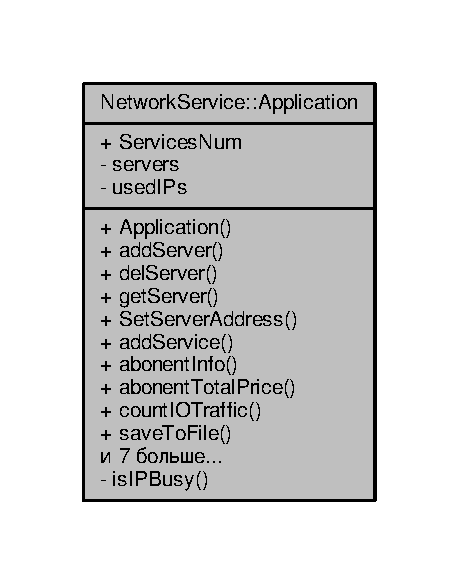
\includegraphics[width=220pt]{class_network_service_1_1_application__coll__graph}
\end{center}
\end{figure}
\subsection*{Открытые типы}
\begin{DoxyCompactItemize}
\item 
typedef \hyperlink{class_network_service_1_1_server}{Server} \hyperlink{class_network_service_1_1_application_a4cbe718a4ebf378cf75cc55fe015177a}{index\+T}
\begin{DoxyCompactList}\small\item\em Определение типа для работы итератора \end{DoxyCompactList}\item 
typedef \hyperlink{class_network_service_1_1_my_iterator}{My\+Iterator}$<$ \hyperlink{class_network_service_1_1_application}{Application} $>$ \hyperlink{class_network_service_1_1_application_a206937019d86d3391a209e9883b44f7b}{Iterator}
\begin{DoxyCompactList}\small\item\em Специализация шаблонного типа \hyperlink{class_network_service_1_1_my_iterator}{My\+Iterator}. \end{DoxyCompactList}\item 
typedef \hyperlink{class_network_service_1_1_my_const_iterator}{My\+Const\+Iterator}$<$ \hyperlink{class_network_service_1_1_application}{Application} $>$ \hyperlink{class_network_service_1_1_application_a51fff3b7cce6bf84c2edbd887c0cac45}{Const\+Iterator}
\begin{DoxyCompactList}\small\item\em Специализация шаблонного типа \hyperlink{class_network_service_1_1_my_const_iterator}{My\+Const\+Iterator}. \end{DoxyCompactList}\end{DoxyCompactItemize}
\subsection*{Открытые члены}
\begin{DoxyCompactItemize}
\item 
\hyperlink{class_network_service_1_1_application_abfad2c23a7824c984a7ee1e6141d732b}{Application} ()
\item 
void \hyperlink{class_network_service_1_1_application_a7c718890bcaa6cce31f29c1ae7e69b81}{add\+Server} (ulong addr, std\+::string name, ulong costpermin, ulong costpermb)
\begin{DoxyCompactList}\small\item\em Добавление нового сервера в таблицу \end{DoxyCompactList}\item 
void \hyperlink{class_network_service_1_1_application_ad09e462bffd3345934a1e3f3eca89774}{del\+Server} (ulong addr)
\begin{DoxyCompactList}\small\item\em Удаление сервера из таблицы \end{DoxyCompactList}\item 
\hyperlink{class_network_service_1_1_server}{Server} \& \hyperlink{class_network_service_1_1_application_acb73429fd01baca7eb138c316f05c97a}{get\+Server} (ulong addr)
\begin{DoxyCompactList}\small\item\em Находит сервер в таблице по адресу \end{DoxyCompactList}\item 
void \hyperlink{class_network_service_1_1_application_a7b18fb99b391286a0cf85c3c731b5982}{Set\+Server\+Address} (\hyperlink{class_network_service_1_1_server}{Server} \&srv, ulong newaddr)
\begin{DoxyCompactList}\small\item\em Изменение I\+P адреса сервера \end{DoxyCompactList}\item 
void \hyperlink{class_network_service_1_1_application_a31f7383eb1d003932ca6d3111571ef2e}{add\+Service} (ulong serveraddr, ulong abonentaddr, \hyperlink{class_network_service_1_1_service_descriptor}{Service\+Descriptor} $\ast$sdesc)
\begin{DoxyCompactList}\small\item\em Добавление записи об оказанной услуге в \char`\"{}таблицу связи\char`\"{} сервера \end{DoxyCompactList}\item 
std\+::vector$<$ std\+::string $>$ \hyperlink{class_network_service_1_1_application_a0b064e8f7ab3a8932a610f53713e12ab}{abonent\+Info} (ulong abonentaddr) const 
\begin{DoxyCompactList}\small\item\em Cбор информации о количестве переданных данных и длительности связи для абонента \end{DoxyCompactList}\item 
ulong \hyperlink{class_network_service_1_1_application_ab44d0123e96ef44496aab54effc42281}{abonent\+Total\+Price} (ulong abonentaddr) const 
\begin{DoxyCompactList}\small\item\em Считает итоговую стоимость оказанных услуг абонента \end{DoxyCompactList}\item 
std\+::pair$<$ ulong, ulong $>$ \hyperlink{class_network_service_1_1_application_a52c98b58888cda1930b1d88d99ab7af7}{count\+I\+O\+Traffic} () const 
\begin{DoxyCompactList}\small\item\em Считает количество переданных данных и количество полученных данных \end{DoxyCompactList}\item 
void \hyperlink{class_network_service_1_1_application_a670578bac65348d3c604fdf53585102b}{save\+To\+File} (std\+::string \&path)
\begin{DoxyCompactList}\small\item\em Сохраняет записи в J\+S\+O\+N формате в текстовый файл \end{DoxyCompactList}\item 
void \hyperlink{class_network_service_1_1_application_ab86f830805a3b9ab2909ea65f7eb48b8}{read\+From\+File} (std\+::string \&path)
\begin{DoxyCompactList}\small\item\em Считывает информацию о серверах и оказанных услугах из текстового файла, содержащего J\+S\+O\+N представление \end{DoxyCompactList}\item 
\hyperlink{class_network_service_1_1_application_a206937019d86d3391a209e9883b44f7b}{Iterator} \hyperlink{class_network_service_1_1_application_af79bea7489f0192a631af1477290af14}{begin} ()
\begin{DoxyCompactList}\small\item\em Итератор, указывающий на первый элемент таблицы \end{DoxyCompactList}\item 
\hyperlink{class_network_service_1_1_application_a51fff3b7cce6bf84c2edbd887c0cac45}{Const\+Iterator} \hyperlink{class_network_service_1_1_application_a2d3762c2bc3f66e96b1295ec584f779d}{begin} () const 
\begin{DoxyCompactList}\small\item\em Константный итератор, указывающий на первый элемент таблицы \end{DoxyCompactList}\item 
\hyperlink{class_network_service_1_1_application_a206937019d86d3391a209e9883b44f7b}{Iterator} \hyperlink{class_network_service_1_1_application_ab0fcfd1baa6f19b018ad6e8ab7ca122c}{end} ()
\begin{DoxyCompactList}\small\item\em Итератор, указывающий на конец таблицы (индекс, равный размеру) \end{DoxyCompactList}\item 
\hyperlink{class_network_service_1_1_application_a51fff3b7cce6bf84c2edbd887c0cac45}{Const\+Iterator} \hyperlink{class_network_service_1_1_application_ae464b274be530d8d8a546488780a077e}{end} () const 
\begin{DoxyCompactList}\small\item\em Константный итератор, указывающий на конец таблицы (индекс, равный размеру) \end{DoxyCompactList}\item 
\hyperlink{class_network_service_1_1_server}{Server} \& \hyperlink{class_network_service_1_1_application_a6dba76630cbd2d6863d2331475a18518}{operator\mbox{[}$\,$\mbox{]}} (uint index)
\begin{DoxyCompactList}\small\item\em Оператор индексирования таблицы серверов \end{DoxyCompactList}\item 
virtual \hyperlink{class_network_service_1_1_application_a5f806355ef363880214dc158c24951d6}{$\sim$\+Application} ()
\end{DoxyCompactItemize}
\subsection*{Открытые атрибуты}
\begin{DoxyCompactItemize}
\item 
const uint \hyperlink{class_network_service_1_1_application_a95664d256ae9f339502b82b462d46365}{Services\+Num} = 3
\begin{DoxyCompactList}\small\item\em Количество возможных вариантов сервиса (почта,файлы,сеть) \end{DoxyCompactList}\end{DoxyCompactItemize}
\subsection*{Закрытые члены}
\begin{DoxyCompactItemize}
\item 
bool \hyperlink{class_network_service_1_1_application_a3bc3a188eb55fad7bdd9be11af54391b}{is\+I\+P\+Busy} (ulong addr) const 
\begin{DoxyCompactList}\small\item\em Проверка, занят ли адрес \end{DoxyCompactList}\end{DoxyCompactItemize}
\subsection*{Закрытые данные}
\begin{DoxyCompactItemize}
\item 
std\+::vector$<$ \hyperlink{class_network_service_1_1_application_a4cbe718a4ebf378cf75cc55fe015177a}{index\+T} $>$ \hyperlink{class_network_service_1_1_application_af499fff927e0ee95480eeac2f4bb464b}{servers}
\begin{DoxyCompactList}\small\item\em Таблица серверов \end{DoxyCompactList}\item 
std\+::vector$<$ ulong $>$ \hyperlink{class_network_service_1_1_application_a9709635bcf03ef131a655ca1c58efa6b}{used\+I\+Ps}
\begin{DoxyCompactList}\small\item\em Таблица использованных адресов \end{DoxyCompactList}\end{DoxyCompactItemize}
\subsection*{Друзья}
\begin{DoxyCompactItemize}
\item 
class \hyperlink{class_network_service_1_1_application_ad14d365afc30a96b618aab998f4572e5}{My\+Iterator$<$ Application $>$}
\end{DoxyCompactItemize}


\subsection{Подробное описание}
Класс, реализующий работу приложения 

Отвечает за взаимодействия прикладной программы с библиотекой 

\subsection{Определения типов}
\hypertarget{class_network_service_1_1_application_a51fff3b7cce6bf84c2edbd887c0cac45}{}\index{Network\+Service\+::\+Application@{Network\+Service\+::\+Application}!Const\+Iterator@{Const\+Iterator}}
\index{Const\+Iterator@{Const\+Iterator}!Network\+Service\+::\+Application@{Network\+Service\+::\+Application}}
\subsubsection[{Const\+Iterator}]{\setlength{\rightskip}{0pt plus 5cm}typedef {\bf My\+Const\+Iterator}$<${\bf Application}$>$ {\bf Network\+Service\+::\+Application\+::\+Const\+Iterator}}\label{class_network_service_1_1_application_a51fff3b7cce6bf84c2edbd887c0cac45}


Специализация шаблонного типа \hyperlink{class_network_service_1_1_my_const_iterator}{My\+Const\+Iterator}. 

\hypertarget{class_network_service_1_1_application_a4cbe718a4ebf378cf75cc55fe015177a}{}\index{Network\+Service\+::\+Application@{Network\+Service\+::\+Application}!index\+T@{index\+T}}
\index{index\+T@{index\+T}!Network\+Service\+::\+Application@{Network\+Service\+::\+Application}}
\subsubsection[{index\+T}]{\setlength{\rightskip}{0pt plus 5cm}typedef {\bf Server} {\bf Network\+Service\+::\+Application\+::index\+T}}\label{class_network_service_1_1_application_a4cbe718a4ebf378cf75cc55fe015177a}


Определение типа для работы итератора 

\hypertarget{class_network_service_1_1_application_a206937019d86d3391a209e9883b44f7b}{}\index{Network\+Service\+::\+Application@{Network\+Service\+::\+Application}!Iterator@{Iterator}}
\index{Iterator@{Iterator}!Network\+Service\+::\+Application@{Network\+Service\+::\+Application}}
\subsubsection[{Iterator}]{\setlength{\rightskip}{0pt plus 5cm}typedef {\bf My\+Iterator}$<${\bf Application}$>$ {\bf Network\+Service\+::\+Application\+::\+Iterator}}\label{class_network_service_1_1_application_a206937019d86d3391a209e9883b44f7b}


Специализация шаблонного типа \hyperlink{class_network_service_1_1_my_iterator}{My\+Iterator}. 



\subsection{Конструктор(ы)}
\hypertarget{class_network_service_1_1_application_abfad2c23a7824c984a7ee1e6141d732b}{}\index{Network\+Service\+::\+Application@{Network\+Service\+::\+Application}!Application@{Application}}
\index{Application@{Application}!Network\+Service\+::\+Application@{Network\+Service\+::\+Application}}
\subsubsection[{Application}]{\setlength{\rightskip}{0pt plus 5cm}Network\+Service\+::\+Application\+::\+Application (
\begin{DoxyParamCaption}
{}
\end{DoxyParamCaption}
)}\label{class_network_service_1_1_application_abfad2c23a7824c984a7ee1e6141d732b}
\hypertarget{class_network_service_1_1_application_a5f806355ef363880214dc158c24951d6}{}\index{Network\+Service\+::\+Application@{Network\+Service\+::\+Application}!````~Application@{$\sim$\+Application}}
\index{````~Application@{$\sim$\+Application}!Network\+Service\+::\+Application@{Network\+Service\+::\+Application}}
\subsubsection[{$\sim$\+Application}]{\setlength{\rightskip}{0pt plus 5cm}virtual Network\+Service\+::\+Application\+::$\sim$\+Application (
\begin{DoxyParamCaption}
{}
\end{DoxyParamCaption}
)\hspace{0.3cm}{\ttfamily [virtual]}}\label{class_network_service_1_1_application_a5f806355ef363880214dc158c24951d6}


\subsection{Методы}
\hypertarget{class_network_service_1_1_application_a0b064e8f7ab3a8932a610f53713e12ab}{}\index{Network\+Service\+::\+Application@{Network\+Service\+::\+Application}!abonent\+Info@{abonent\+Info}}
\index{abonent\+Info@{abonent\+Info}!Network\+Service\+::\+Application@{Network\+Service\+::\+Application}}
\subsubsection[{abonent\+Info}]{\setlength{\rightskip}{0pt plus 5cm}std\+::vector$<$ std\+::string $>$ Application\+::abonent\+Info (
\begin{DoxyParamCaption}
\item[{ulong}]{abonentaddr}
\end{DoxyParamCaption}
) const}\label{class_network_service_1_1_application_a0b064e8f7ab3a8932a610f53713e12ab}


Cбор информации о количестве переданных данных и длительности связи для абонента 


\begin{DoxyParams}{Аргументы}
{\em abonentaddr} & I\+P адрес абонента \\
\hline
\end{DoxyParams}
\begin{DoxyReturn}{Возвращает}
vector из string -\/ текстовое представление собранной информации 
\end{DoxyReturn}

\begin{DoxyExceptions}{Исключения}
{\em invalid\+\_\+argument} & если адрес абонента неверен или не найден\\
\hline
\end{DoxyExceptions}
Метод проходит по всем серверам и их таблицам связи, используя итераторы, собирая информацию во \char`\"{}временную\char`\"{} коллекцию следующего вида 
\begin{DoxyCodeInclude}
    std::vector<std::pair<ulong,ulong>> counter;
    counter.reserve(\hyperlink{class_network_service_1_1_application_a95664d256ae9f339502b82b462d46365}{ServicesNum});
\end{DoxyCodeInclude}
Первый элемент пары -\/ суммарный траффик для сервиса (передано+получено), Второй -\/ Общая длительность связи для сервиса (не для всех сервисов) Вектор result резервируется для 3-\/х сервисов \mbox{[}countervec\mbox{]}

\mbox{[}countervec\mbox{]} \hypertarget{class_network_service_1_1_application_ab44d0123e96ef44496aab54effc42281}{}\index{Network\+Service\+::\+Application@{Network\+Service\+::\+Application}!abonent\+Total\+Price@{abonent\+Total\+Price}}
\index{abonent\+Total\+Price@{abonent\+Total\+Price}!Network\+Service\+::\+Application@{Network\+Service\+::\+Application}}
\subsubsection[{abonent\+Total\+Price}]{\setlength{\rightskip}{0pt plus 5cm}ulong Application\+::abonent\+Total\+Price (
\begin{DoxyParamCaption}
\item[{ulong}]{abonentaddr}
\end{DoxyParamCaption}
) const}\label{class_network_service_1_1_application_ab44d0123e96ef44496aab54effc42281}


Считает итоговую стоимость оказанных услуг абонента 


\begin{DoxyParams}{Аргументы}
{\em abonentaddr} & I\+P адрес абонента \\
\hline
\end{DoxyParams}
\begin{DoxyReturn}{Возвращает}
Итоговая стоимость
\end{DoxyReturn}
Метод проходит по всем серверам и их \char`\"{}таблицам связи\char`\"{} (используются итераторы), вызывая для каждой записи виртуальную функцию calculate\+Price() и прибавляя ее результат к итоговому \hypertarget{class_network_service_1_1_application_a7c718890bcaa6cce31f29c1ae7e69b81}{}\index{Network\+Service\+::\+Application@{Network\+Service\+::\+Application}!add\+Server@{add\+Server}}
\index{add\+Server@{add\+Server}!Network\+Service\+::\+Application@{Network\+Service\+::\+Application}}
\subsubsection[{add\+Server}]{\setlength{\rightskip}{0pt plus 5cm}void Application\+::add\+Server (
\begin{DoxyParamCaption}
\item[{ulong}]{addr, }
\item[{std\+::string}]{name, }
\item[{ulong}]{costpermin, }
\item[{ulong}]{costpermb}
\end{DoxyParamCaption}
)}\label{class_network_service_1_1_application_a7c718890bcaa6cce31f29c1ae7e69b81}


Добавление нового сервера в таблицу 


\begin{DoxyParams}{Аргументы}
{\em addr} & I\+P адрес сервера \\
\hline
{\em name} & Имя сервера \\
\hline
{\em costpermin} & Стоимость 1 минуты связи \\
\hline
{\em costpermb} & Стоимость 1\+M\+B переданных данных \\
\hline
\end{DoxyParams}

\begin{DoxyExceptions}{Исключения}
{\em invalid\+\_\+argument} & если I\+P адрес сервера неверный \\
\hline
{\em logic\+\_\+error} & если I\+P адрес занят(используется)\\
\hline
\end{DoxyExceptions}
Метод добавляет новый сервер в таблицу, в случае успешного добавления сервера I\+P адрес добавляется в таблицу используемых адресов \hypertarget{class_network_service_1_1_application_a31f7383eb1d003932ca6d3111571ef2e}{}\index{Network\+Service\+::\+Application@{Network\+Service\+::\+Application}!add\+Service@{add\+Service}}
\index{add\+Service@{add\+Service}!Network\+Service\+::\+Application@{Network\+Service\+::\+Application}}
\subsubsection[{add\+Service}]{\setlength{\rightskip}{0pt plus 5cm}void Application\+::add\+Service (
\begin{DoxyParamCaption}
\item[{ulong}]{serveraddr, }
\item[{ulong}]{abonentaddr, }
\item[{{\bf Service\+Descriptor} $\ast$}]{sdesc}
\end{DoxyParamCaption}
)}\label{class_network_service_1_1_application_a31f7383eb1d003932ca6d3111571ef2e}


Добавление записи об оказанной услуге в \char`\"{}таблицу связи\char`\"{} сервера 


\begin{DoxyParams}{Аргументы}
{\em serveraddr} & I\+P адрес сервера \\
\hline
{\em abonentaddr} & I\+P адрес клиента \\
\hline
{\em sdesc} & Указатель на описатель сервиса (полиморфный \hyperlink{class_network_service_1_1_service_descriptor}{Service\+Descriptor}) \\
\hline
\end{DoxyParams}

\begin{DoxyExceptions}{Исключения}
{\em invalid\+\_\+argument} & Если\+:
\begin{DoxyItemize}
\item Неверный I\+P сервера
\item Неверный I\+P клиента
\item В качестве указателя на \hyperlink{class_network_service_1_1_service_descriptor}{Service\+Descriptor} передан нулевой указатель
\end{DoxyItemize}\\
\hline
\end{DoxyExceptions}
Метод ищет сервер в таблице серверов и добавляет в его \char`\"{}таблицу связи\char`\"{} информацию об оказанной услуге. Также метод добавляет I\+P адрес клиента в таблицу занятых адресов, если такого адреса там еще нет \hypertarget{class_network_service_1_1_application_af79bea7489f0192a631af1477290af14}{}\index{Network\+Service\+::\+Application@{Network\+Service\+::\+Application}!begin@{begin}}
\index{begin@{begin}!Network\+Service\+::\+Application@{Network\+Service\+::\+Application}}
\subsubsection[{begin}]{\setlength{\rightskip}{0pt plus 5cm}{\bf Application\+::\+Iterator} Application\+::begin (
\begin{DoxyParamCaption}
{}
\end{DoxyParamCaption}
)}\label{class_network_service_1_1_application_af79bea7489f0192a631af1477290af14}


Итератор, указывающий на первый элемент таблицы 

\begin{DoxyReturn}{Возвращает}
объект Iterator 
\end{DoxyReturn}
\hypertarget{class_network_service_1_1_application_a2d3762c2bc3f66e96b1295ec584f779d}{}\index{Network\+Service\+::\+Application@{Network\+Service\+::\+Application}!begin@{begin}}
\index{begin@{begin}!Network\+Service\+::\+Application@{Network\+Service\+::\+Application}}
\subsubsection[{begin}]{\setlength{\rightskip}{0pt plus 5cm}{\bf Application\+::\+Const\+Iterator} Application\+::begin (
\begin{DoxyParamCaption}
{}
\end{DoxyParamCaption}
) const}\label{class_network_service_1_1_application_a2d3762c2bc3f66e96b1295ec584f779d}


Константный итератор, указывающий на первый элемент таблицы 

\begin{DoxyReturn}{Возвращает}
объект Const\+Iterator 
\end{DoxyReturn}
\hypertarget{class_network_service_1_1_application_a52c98b58888cda1930b1d88d99ab7af7}{}\index{Network\+Service\+::\+Application@{Network\+Service\+::\+Application}!count\+I\+O\+Traffic@{count\+I\+O\+Traffic}}
\index{count\+I\+O\+Traffic@{count\+I\+O\+Traffic}!Network\+Service\+::\+Application@{Network\+Service\+::\+Application}}
\subsubsection[{count\+I\+O\+Traffic}]{\setlength{\rightskip}{0pt plus 5cm}std\+::pair$<$ ulong, ulong $>$ Application\+::count\+I\+O\+Traffic (
\begin{DoxyParamCaption}
{}
\end{DoxyParamCaption}
) const}\label{class_network_service_1_1_application_a52c98b58888cda1930b1d88d99ab7af7}


Считает количество переданных данных и количество полученных данных 

\begin{DoxyReturn}{Возвращает}
пара значений\+: первое -\/ количество переданных данных, второе -\/ количество полученных
\end{DoxyReturn}
Метод проходит по всем серверам и их \char`\"{}таблицам связи\char`\"{} (используются итераторы), считывает количество данных и направление их передачи, добавляя к результату \hypertarget{class_network_service_1_1_application_ad09e462bffd3345934a1e3f3eca89774}{}\index{Network\+Service\+::\+Application@{Network\+Service\+::\+Application}!del\+Server@{del\+Server}}
\index{del\+Server@{del\+Server}!Network\+Service\+::\+Application@{Network\+Service\+::\+Application}}
\subsubsection[{del\+Server}]{\setlength{\rightskip}{0pt plus 5cm}void Application\+::del\+Server (
\begin{DoxyParamCaption}
\item[{ulong}]{addr}
\end{DoxyParamCaption}
)}\label{class_network_service_1_1_application_ad09e462bffd3345934a1e3f3eca89774}


Удаление сервера из таблицы 


\begin{DoxyParams}{Аргументы}
{\em addr} & I\+P адрес удаляемого сервера \\
\hline
\end{DoxyParams}

\begin{DoxyExceptions}{Исключения}
{\em invalid\+\_\+argument} & если I\+P неверный или сервер с таким адресом не был наиден\\
\hline
\end{DoxyExceptions}
Метод удаляет сервер из таблицы серверов, также I\+P адрес удаляется из таблицы использованных адресов \hypertarget{class_network_service_1_1_application_ab0fcfd1baa6f19b018ad6e8ab7ca122c}{}\index{Network\+Service\+::\+Application@{Network\+Service\+::\+Application}!end@{end}}
\index{end@{end}!Network\+Service\+::\+Application@{Network\+Service\+::\+Application}}
\subsubsection[{end}]{\setlength{\rightskip}{0pt plus 5cm}{\bf Application\+::\+Iterator} Application\+::end (
\begin{DoxyParamCaption}
{}
\end{DoxyParamCaption}
)}\label{class_network_service_1_1_application_ab0fcfd1baa6f19b018ad6e8ab7ca122c}


Итератор, указывающий на конец таблицы (индекс, равный размеру) 

\begin{DoxyReturn}{Возвращает}
объект Iterator 
\end{DoxyReturn}
\hypertarget{class_network_service_1_1_application_ae464b274be530d8d8a546488780a077e}{}\index{Network\+Service\+::\+Application@{Network\+Service\+::\+Application}!end@{end}}
\index{end@{end}!Network\+Service\+::\+Application@{Network\+Service\+::\+Application}}
\subsubsection[{end}]{\setlength{\rightskip}{0pt plus 5cm}{\bf Application\+::\+Const\+Iterator} Application\+::end (
\begin{DoxyParamCaption}
{}
\end{DoxyParamCaption}
) const}\label{class_network_service_1_1_application_ae464b274be530d8d8a546488780a077e}


Константный итератор, указывающий на конец таблицы (индекс, равный размеру) 

\begin{DoxyReturn}{Возвращает}
объект Const\+Iterator 
\end{DoxyReturn}
\hypertarget{class_network_service_1_1_application_acb73429fd01baca7eb138c316f05c97a}{}\index{Network\+Service\+::\+Application@{Network\+Service\+::\+Application}!get\+Server@{get\+Server}}
\index{get\+Server@{get\+Server}!Network\+Service\+::\+Application@{Network\+Service\+::\+Application}}
\subsubsection[{get\+Server}]{\setlength{\rightskip}{0pt plus 5cm}{\bf Server} \& Application\+::get\+Server (
\begin{DoxyParamCaption}
\item[{ulong}]{addr}
\end{DoxyParamCaption}
)}\label{class_network_service_1_1_application_acb73429fd01baca7eb138c316f05c97a}


Находит сервер в таблице по адресу 


\begin{DoxyParams}{Аргументы}
{\em addr} & I\+P адрес предполагаемого сервера \\
\hline
\end{DoxyParams}
\begin{DoxyReturn}{Возвращает}
ссылка на объект \hyperlink{class_network_service_1_1_server}{Server} 
\end{DoxyReturn}

\begin{DoxyExceptions}{Исключения}
{\em invalid\+\_\+argument} & если I\+P адрес неверный или сервера с таким адресом не найдено \\
\hline
\end{DoxyExceptions}
\hypertarget{class_network_service_1_1_application_a3bc3a188eb55fad7bdd9be11af54391b}{}\index{Network\+Service\+::\+Application@{Network\+Service\+::\+Application}!is\+I\+P\+Busy@{is\+I\+P\+Busy}}
\index{is\+I\+P\+Busy@{is\+I\+P\+Busy}!Network\+Service\+::\+Application@{Network\+Service\+::\+Application}}
\subsubsection[{is\+I\+P\+Busy}]{\setlength{\rightskip}{0pt plus 5cm}bool Application\+::is\+I\+P\+Busy (
\begin{DoxyParamCaption}
\item[{ulong}]{addr}
\end{DoxyParamCaption}
) const\hspace{0.3cm}{\ttfamily [private]}}\label{class_network_service_1_1_application_a3bc3a188eb55fad7bdd9be11af54391b}


Проверка, занят ли адрес 


\begin{DoxyParams}{Аргументы}
{\em addr} & Проверяемый адрес \\
\hline
\end{DoxyParams}
\begin{DoxyReturn}{Возвращает}
true, если занят, false, если свободен
\end{DoxyReturn}
Метод ищет проверяемый адрес в таблице используемых адресов \hypertarget{class_network_service_1_1_application_a6dba76630cbd2d6863d2331475a18518}{}\index{Network\+Service\+::\+Application@{Network\+Service\+::\+Application}!operator\mbox{[}$\,$\mbox{]}@{operator[]}}
\index{operator\mbox{[}$\,$\mbox{]}@{operator[]}!Network\+Service\+::\+Application@{Network\+Service\+::\+Application}}
\subsubsection[{operator[]}]{\setlength{\rightskip}{0pt plus 5cm}{\bf Server} \& Application\+::operator\mbox{[}$\,$\mbox{]} (
\begin{DoxyParamCaption}
\item[{uint}]{index}
\end{DoxyParamCaption}
)}\label{class_network_service_1_1_application_a6dba76630cbd2d6863d2331475a18518}


Оператор индексирования таблицы серверов 


\begin{DoxyParams}{Аргументы}
{\em index} & Индекс \\
\hline
\end{DoxyParams}
\begin{DoxyReturn}{Возвращает}
Ссылка на объект \hyperlink{class_network_service_1_1_server}{Server} 
\end{DoxyReturn}

\begin{DoxyExceptions}{Исключения}
{\em invalid\+\_\+argument} & если index больше, чем размер таблицы\\
\hline
\end{DoxyExceptions}
Метод использует перегруженный оператор для \mbox{[}\mbox{]} для таблицы серверов. Метод необходим для работы итераторов \hypertarget{class_network_service_1_1_application_ab86f830805a3b9ab2909ea65f7eb48b8}{}\index{Network\+Service\+::\+Application@{Network\+Service\+::\+Application}!read\+From\+File@{read\+From\+File}}
\index{read\+From\+File@{read\+From\+File}!Network\+Service\+::\+Application@{Network\+Service\+::\+Application}}
\subsubsection[{read\+From\+File}]{\setlength{\rightskip}{0pt plus 5cm}void Application\+::read\+From\+File (
\begin{DoxyParamCaption}
\item[{std\+::string \&}]{path}
\end{DoxyParamCaption}
)}\label{class_network_service_1_1_application_ab86f830805a3b9ab2909ea65f7eb48b8}


Считывает информацию о серверах и оказанных услугах из текстового файла, содержащего J\+S\+O\+N представление 


\begin{DoxyParams}{Аргументы}
{\em path} & Путь к исходному файлу \\
\hline
\end{DoxyParams}

\begin{DoxyExceptions}{Исключения}
{\em invalid\+\_\+argument} & если не удалось открыть файл на чтение \\
\hline
{\em logic\+\_\+error} & в случае ошибки разбора\\
\hline
\end{DoxyExceptions}
Метод разбирает J\+S\+O\+N представление, взятое из файла, восстанавливая информацию о серверах и оказанных услугах \hypertarget{class_network_service_1_1_application_a670578bac65348d3c604fdf53585102b}{}\index{Network\+Service\+::\+Application@{Network\+Service\+::\+Application}!save\+To\+File@{save\+To\+File}}
\index{save\+To\+File@{save\+To\+File}!Network\+Service\+::\+Application@{Network\+Service\+::\+Application}}
\subsubsection[{save\+To\+File}]{\setlength{\rightskip}{0pt plus 5cm}void Application\+::save\+To\+File (
\begin{DoxyParamCaption}
\item[{std\+::string \&}]{path}
\end{DoxyParamCaption}
)}\label{class_network_service_1_1_application_a670578bac65348d3c604fdf53585102b}


Сохраняет записи в J\+S\+O\+N формате в текстовый файл 


\begin{DoxyParams}{Аргументы}
{\em path} & Путь к файлу назначения \\
\hline
\end{DoxyParams}

\begin{DoxyExceptions}{Исключения}
{\em logic\+\_\+error} & в случае ошибки открытия файла на запись\\
\hline
\end{DoxyExceptions}
Метод проходит по всем серверам и их \char`\"{}таблицам связи\char`\"{} (используются итераторы), сохраняя информацию в J\+S\+O\+N формате в текстовый файл \hypertarget{class_network_service_1_1_application_a7b18fb99b391286a0cf85c3c731b5982}{}\index{Network\+Service\+::\+Application@{Network\+Service\+::\+Application}!Set\+Server\+Address@{Set\+Server\+Address}}
\index{Set\+Server\+Address@{Set\+Server\+Address}!Network\+Service\+::\+Application@{Network\+Service\+::\+Application}}
\subsubsection[{Set\+Server\+Address}]{\setlength{\rightskip}{0pt plus 5cm}void Application\+::\+Set\+Server\+Address (
\begin{DoxyParamCaption}
\item[{{\bf Server} \&}]{srv, }
\item[{ulong}]{newaddr}
\end{DoxyParamCaption}
)}\label{class_network_service_1_1_application_a7b18fb99b391286a0cf85c3c731b5982}


Изменение I\+P адреса сервера 


\begin{DoxyParams}{Аргументы}
{\em srv} & Ссылка на объект \hyperlink{class_network_service_1_1_server}{Server} \\
\hline
{\em newaddr} & Новый адрес \\
\hline
\end{DoxyParams}

\begin{DoxyExceptions}{Исключения}
{\em invalid\+\_\+argument} & если адрес неверный или занят\\
\hline
\end{DoxyExceptions}
Метод меняет своиство address у объекта \hyperlink{class_network_service_1_1_server}{Server}, проверяя новый адрес на занятость по таблице занятых адресов и на правильность 

\subsection{Документация по друзьям класса и функциям, относящимся к классу}
\hypertarget{class_network_service_1_1_application_ad14d365afc30a96b618aab998f4572e5}{}\index{Network\+Service\+::\+Application@{Network\+Service\+::\+Application}!My\+Iterator$<$ Application $>$@{My\+Iterator$<$ Application $>$}}
\index{My\+Iterator$<$ Application $>$@{My\+Iterator$<$ Application $>$}!Network\+Service\+::\+Application@{Network\+Service\+::\+Application}}
\subsubsection[{My\+Iterator$<$ Application $>$}]{\setlength{\rightskip}{0pt plus 5cm}friend class {\bf My\+Iterator}$<$ {\bf Application} $>$\hspace{0.3cm}{\ttfamily [friend]}}\label{class_network_service_1_1_application_ad14d365afc30a96b618aab998f4572e5}


\subsection{Данные класса}
\hypertarget{class_network_service_1_1_application_af499fff927e0ee95480eeac2f4bb464b}{}\index{Network\+Service\+::\+Application@{Network\+Service\+::\+Application}!servers@{servers}}
\index{servers@{servers}!Network\+Service\+::\+Application@{Network\+Service\+::\+Application}}
\subsubsection[{servers}]{\setlength{\rightskip}{0pt plus 5cm}std\+::vector$<${\bf index\+T}$>$ Network\+Service\+::\+Application\+::servers\hspace{0.3cm}{\ttfamily [private]}}\label{class_network_service_1_1_application_af499fff927e0ee95480eeac2f4bb464b}


Таблица серверов 

\hypertarget{class_network_service_1_1_application_a95664d256ae9f339502b82b462d46365}{}\index{Network\+Service\+::\+Application@{Network\+Service\+::\+Application}!Services\+Num@{Services\+Num}}
\index{Services\+Num@{Services\+Num}!Network\+Service\+::\+Application@{Network\+Service\+::\+Application}}
\subsubsection[{Services\+Num}]{\setlength{\rightskip}{0pt plus 5cm}const uint Network\+Service\+::\+Application\+::\+Services\+Num = 3}\label{class_network_service_1_1_application_a95664d256ae9f339502b82b462d46365}


Количество возможных вариантов сервиса (почта,файлы,сеть) 

\hypertarget{class_network_service_1_1_application_a9709635bcf03ef131a655ca1c58efa6b}{}\index{Network\+Service\+::\+Application@{Network\+Service\+::\+Application}!used\+I\+Ps@{used\+I\+Ps}}
\index{used\+I\+Ps@{used\+I\+Ps}!Network\+Service\+::\+Application@{Network\+Service\+::\+Application}}
\subsubsection[{used\+I\+Ps}]{\setlength{\rightskip}{0pt plus 5cm}std\+::vector$<$ulong$>$ Network\+Service\+::\+Application\+::used\+I\+Ps\hspace{0.3cm}{\ttfamily [private]}}\label{class_network_service_1_1_application_a9709635bcf03ef131a655ca1c58efa6b}


Таблица использованных адресов 



Объявления и описания членов классов находятся в файлах\+:\begin{DoxyCompactItemize}
\item 
Network\+Service\+Lib/\hyperlink{application_8h}{application.\+h}\item 
Network\+Service\+Lib/\hyperlink{application_8cpp}{application.\+cpp}\end{DoxyCompactItemize}

\hypertarget{class_network_service_1_1_file_descriptor}{}\section{Класс Network\+Service\+:\+:File\+Descriptor}
\label{class_network_service_1_1_file_descriptor}\index{Network\+Service\+::\+File\+Descriptor@{Network\+Service\+::\+File\+Descriptor}}


Класс, описывающий сервис \char`\"{}файл\char`\"{}.  




{\ttfamily \#include $<$filedescriptor.\+h$>$}



Граф наследования\+:Network\+Service\+:\+:File\+Descriptor\+:\nopagebreak
\begin{figure}[H]
\begin{center}
\leavevmode
\includegraphics[height=550pt]{class_network_service_1_1_file_descriptor__inherit__graph}
\end{center}
\end{figure}


Граф связей класса Network\+Service\+:\+:File\+Descriptor\+:\nopagebreak
\begin{figure}[H]
\begin{center}
\leavevmode
\includegraphics[height=550pt]{class_network_service_1_1_file_descriptor__coll__graph}
\end{center}
\end{figure}
\subsection*{Открытые члены}
\begin{DoxyCompactItemize}
\item 
\hyperlink{class_network_service_1_1_file_descriptor_a87c067c9340ac785ff7fb7a012ea8bba}{File\+Descriptor} (ulong \hyperlink{class_network_service_1_1_post_descriptor_ae2eef559828a42ec299ab59711f88e59}{traffic}, \hyperlink{namespace_network_service_abe1196dad9e8afcbc5c6b38196ce2c65}{Direction} \hyperlink{class_network_service_1_1_post_descriptor_a04faf66e747b2d4f2d89bf1e92f4ab5c}{direction}, ulong address, \hyperlink{networkservice_8h_ac877dfabb0f4f6a8184aa821b447e81d}{ftimepoint} \&\hyperlink{class_network_service_1_1_service_descriptor_a08bfd17afce0cba1954d30bd76a14df4}{linktime}, \hyperlink{networkservice_8h_a476cc728ef971cba9111c75ea41a760a}{fduration} \&\hyperlink{class_network_service_1_1_file_descriptor_a1ce56aef66c93f0a6a5eebc8d43c4bb8}{linkduration}, \hyperlink{class_network_service_1_1_server}{Server} $\ast$\hyperlink{class_network_service_1_1_service_descriptor_ad504b32ced44a75e0e02ea961d9434c4}{server})
\begin{DoxyCompactList}\small\item\em Создает запись об оказанной услуге, основываясь на параметрах \end{DoxyCompactList}\item 
const \hyperlink{networkservice_8h_a476cc728ef971cba9111c75ea41a760a}{fduration} \& \hyperlink{class_network_service_1_1_file_descriptor_ae77011c643f4d7889a417e6fc91a3c72}{get\+Link\+Duration} () const 
\begin{DoxyCompactList}\small\item\em Получение продолжительности связи \end{DoxyCompactList}\item 
std\+::string \hyperlink{class_network_service_1_1_file_descriptor_a68270f753630bf3ac34c621a56e4f6f7}{get\+Type} () const 
\begin{DoxyCompactList}\small\item\em Получение названия типа услуги \end{DoxyCompactList}\item 
ulong \hyperlink{class_network_service_1_1_file_descriptor_a2c480da1613f7072d3113082d1f8cc54}{calculate\+Price} () const 
\begin{DoxyCompactList}\small\item\em Рассчет стоимости оказанных услуг \end{DoxyCompactList}\item 
virtual \hyperlink{class_network_service_1_1_file_descriptor_aaf3da94e82c4a05406c6872a56701195}{$\sim$\+File\+Descriptor} ()
\end{DoxyCompactItemize}
\subsection*{Защищенные члены}
\begin{DoxyCompactItemize}
\item 
void \hyperlink{class_network_service_1_1_file_descriptor_a2f280462647a42806033a39da3f55528}{set\+Link\+Duration} (\hyperlink{networkservice_8h_a476cc728ef971cba9111c75ea41a760a}{fduration} \&ld)
\begin{DoxyCompactList}\small\item\em Установка длительности связи \end{DoxyCompactList}\end{DoxyCompactItemize}
\subsection*{Закрытые члены}
\begin{DoxyCompactItemize}
\item 
\hyperlink{class_network_service_1_1_file_descriptor_addaf36ba62b80d5a50f6fee2c4d02965}{File\+Descriptor} ()
\end{DoxyCompactItemize}
\subsection*{Закрытые данные}
\begin{DoxyCompactItemize}
\item 
\hyperlink{networkservice_8h_a476cc728ef971cba9111c75ea41a760a}{fduration} \hyperlink{class_network_service_1_1_file_descriptor_a1ce56aef66c93f0a6a5eebc8d43c4bb8}{linkduration}
\end{DoxyCompactItemize}


\subsection{Подробное описание}
Класс, описывающий сервис \char`\"{}файл\char`\"{}. 

Наследуется от \hyperlink{class_network_service_1_1_post_descriptor}{Post\+Descriptor} в связи с большим количеством общих полей 

\subsection{Конструктор(ы)}
\hypertarget{class_network_service_1_1_file_descriptor_addaf36ba62b80d5a50f6fee2c4d02965}{}\index{Network\+Service\+::\+File\+Descriptor@{Network\+Service\+::\+File\+Descriptor}!File\+Descriptor@{File\+Descriptor}}
\index{File\+Descriptor@{File\+Descriptor}!Network\+Service\+::\+File\+Descriptor@{Network\+Service\+::\+File\+Descriptor}}
\subsubsection[{File\+Descriptor}]{\setlength{\rightskip}{0pt plus 5cm}File\+Descriptor\+::\+File\+Descriptor (
\begin{DoxyParamCaption}
{}
\end{DoxyParamCaption}
)\hspace{0.3cm}{\ttfamily [private]}}\label{class_network_service_1_1_file_descriptor_addaf36ba62b80d5a50f6fee2c4d02965}
\hypertarget{class_network_service_1_1_file_descriptor_a87c067c9340ac785ff7fb7a012ea8bba}{}\index{Network\+Service\+::\+File\+Descriptor@{Network\+Service\+::\+File\+Descriptor}!File\+Descriptor@{File\+Descriptor}}
\index{File\+Descriptor@{File\+Descriptor}!Network\+Service\+::\+File\+Descriptor@{Network\+Service\+::\+File\+Descriptor}}
\subsubsection[{File\+Descriptor}]{\setlength{\rightskip}{0pt plus 5cm}File\+Descriptor\+::\+File\+Descriptor (
\begin{DoxyParamCaption}
\item[{ulong}]{traffic, }
\item[{{\bf Direction}}]{direction, }
\item[{ulong}]{address, }
\item[{{\bf ftimepoint} \&}]{linktime, }
\item[{{\bf fduration} \&}]{linkduration, }
\item[{{\bf Server} $\ast$}]{server}
\end{DoxyParamCaption}
)}\label{class_network_service_1_1_file_descriptor_a87c067c9340ac785ff7fb7a012ea8bba}


Создает запись об оказанной услуге, основываясь на параметрах 


\begin{DoxyParams}{Аргументы}
{\em traffic} & Количество переданной информации в M\+B \\
\hline
{\em direction} & Направление передачи \\
\hline
{\em address} & Адрес назначения \\
\hline
{\em linktime} & Время связи \\
\hline
{\em linkduration} & Продолжительность связи \\
\hline
{\em server} & Указатель на сервер (объект \hyperlink{class_network_service_1_1_server}{Server}), оказывающий услугу \\
\hline
\end{DoxyParams}
\hypertarget{class_network_service_1_1_file_descriptor_aaf3da94e82c4a05406c6872a56701195}{}\index{Network\+Service\+::\+File\+Descriptor@{Network\+Service\+::\+File\+Descriptor}!````~File\+Descriptor@{$\sim$\+File\+Descriptor}}
\index{````~File\+Descriptor@{$\sim$\+File\+Descriptor}!Network\+Service\+::\+File\+Descriptor@{Network\+Service\+::\+File\+Descriptor}}
\subsubsection[{$\sim$\+File\+Descriptor}]{\setlength{\rightskip}{0pt plus 5cm}File\+Descriptor\+::$\sim$\+File\+Descriptor (
\begin{DoxyParamCaption}
{}
\end{DoxyParamCaption}
)\hspace{0.3cm}{\ttfamily [virtual]}}\label{class_network_service_1_1_file_descriptor_aaf3da94e82c4a05406c6872a56701195}


\subsection{Методы}
\hypertarget{class_network_service_1_1_file_descriptor_a2c480da1613f7072d3113082d1f8cc54}{}\index{Network\+Service\+::\+File\+Descriptor@{Network\+Service\+::\+File\+Descriptor}!calculate\+Price@{calculate\+Price}}
\index{calculate\+Price@{calculate\+Price}!Network\+Service\+::\+File\+Descriptor@{Network\+Service\+::\+File\+Descriptor}}
\subsubsection[{calculate\+Price}]{\setlength{\rightskip}{0pt plus 5cm}ulong File\+Descriptor\+::calculate\+Price (
\begin{DoxyParamCaption}
{}
\end{DoxyParamCaption}
) const\hspace{0.3cm}{\ttfamily [virtual]}}\label{class_network_service_1_1_file_descriptor_a2c480da1613f7072d3113082d1f8cc54}


Рассчет стоимости оказанных услуг 

\begin{DoxyReturn}{Возвращает}
Стоимость оказанных услуг
\end{DoxyReturn}
Рассчет стоимости оказанных услуг, на основании стоимости 1 минуты и 1\+M\+B, установленной сервером 

Переопределяет метод предка \hyperlink{class_network_service_1_1_post_descriptor_ae88dfdc2d12299b6d3b14786d16e3251}{Network\+Service\+::\+Post\+Descriptor}.

\hypertarget{class_network_service_1_1_file_descriptor_ae77011c643f4d7889a417e6fc91a3c72}{}\index{Network\+Service\+::\+File\+Descriptor@{Network\+Service\+::\+File\+Descriptor}!get\+Link\+Duration@{get\+Link\+Duration}}
\index{get\+Link\+Duration@{get\+Link\+Duration}!Network\+Service\+::\+File\+Descriptor@{Network\+Service\+::\+File\+Descriptor}}
\subsubsection[{get\+Link\+Duration}]{\setlength{\rightskip}{0pt plus 5cm}const {\bf fduration} \& File\+Descriptor\+::get\+Link\+Duration (
\begin{DoxyParamCaption}
{}
\end{DoxyParamCaption}
) const}\label{class_network_service_1_1_file_descriptor_ae77011c643f4d7889a417e6fc91a3c72}


Получение продолжительности связи 

\begin{DoxyReturn}{Возвращает}
Ссылка на объект fduration 
\end{DoxyReturn}
\hypertarget{class_network_service_1_1_file_descriptor_a68270f753630bf3ac34c621a56e4f6f7}{}\index{Network\+Service\+::\+File\+Descriptor@{Network\+Service\+::\+File\+Descriptor}!get\+Type@{get\+Type}}
\index{get\+Type@{get\+Type}!Network\+Service\+::\+File\+Descriptor@{Network\+Service\+::\+File\+Descriptor}}
\subsubsection[{get\+Type}]{\setlength{\rightskip}{0pt plus 5cm}std\+::string File\+Descriptor\+::get\+Type (
\begin{DoxyParamCaption}
{}
\end{DoxyParamCaption}
) const\hspace{0.3cm}{\ttfamily [virtual]}}\label{class_network_service_1_1_file_descriptor_a68270f753630bf3ac34c621a56e4f6f7}


Получение названия типа услуги 

\begin{DoxyReturn}{Возвращает}
Название типа услуги (строка \char`\"{}\+File\char`\"{}) 
\end{DoxyReturn}


Переопределяет метод предка \hyperlink{class_network_service_1_1_post_descriptor_a91b6330d604d4866c85c32187f131431}{Network\+Service\+::\+Post\+Descriptor}.

\hypertarget{class_network_service_1_1_file_descriptor_a2f280462647a42806033a39da3f55528}{}\index{Network\+Service\+::\+File\+Descriptor@{Network\+Service\+::\+File\+Descriptor}!set\+Link\+Duration@{set\+Link\+Duration}}
\index{set\+Link\+Duration@{set\+Link\+Duration}!Network\+Service\+::\+File\+Descriptor@{Network\+Service\+::\+File\+Descriptor}}
\subsubsection[{set\+Link\+Duration}]{\setlength{\rightskip}{0pt plus 5cm}void File\+Descriptor\+::set\+Link\+Duration (
\begin{DoxyParamCaption}
\item[{{\bf fduration} \&}]{ld}
\end{DoxyParamCaption}
)\hspace{0.3cm}{\ttfamily [protected]}}\label{class_network_service_1_1_file_descriptor_a2f280462647a42806033a39da3f55528}


Установка длительности связи 


\begin{DoxyParams}{Аргументы}
{\em ld} & Ссылка на объект fduration, содержащий информацию о длительности \\
\hline
\end{DoxyParams}


\subsection{Данные класса}
\hypertarget{class_network_service_1_1_file_descriptor_a1ce56aef66c93f0a6a5eebc8d43c4bb8}{}\index{Network\+Service\+::\+File\+Descriptor@{Network\+Service\+::\+File\+Descriptor}!linkduration@{linkduration}}
\index{linkduration@{linkduration}!Network\+Service\+::\+File\+Descriptor@{Network\+Service\+::\+File\+Descriptor}}
\subsubsection[{linkduration}]{\setlength{\rightskip}{0pt plus 5cm}{\bf fduration} Network\+Service\+::\+File\+Descriptor\+::linkduration\hspace{0.3cm}{\ttfamily [private]}}\label{class_network_service_1_1_file_descriptor_a1ce56aef66c93f0a6a5eebc8d43c4bb8}


Объявления и описания членов классов находятся в файлах\+:\begin{DoxyCompactItemize}
\item 
Network\+Service\+Lib/\hyperlink{filedescriptor_8h}{filedescriptor.\+h}\item 
Network\+Service\+Lib/\hyperlink{filedescriptor_8cpp}{filedescriptor.\+cpp}\end{DoxyCompactItemize}

\hypertarget{class_network_service_1_1_link_table}{}\section{Класс Network\+Service\+:\+:Link\+Table}
\label{class_network_service_1_1_link_table}\index{Network\+Service\+::\+Link\+Table@{Network\+Service\+::\+Link\+Table}}


Класс, реализующий \char`\"{}таблицу связи\char`\"{}.  




{\ttfamily \#include $<$linktable.\+h$>$}



Граф наследования\+:Network\+Service\+:\+:Link\+Table\+:\nopagebreak
\begin{figure}[H]
\begin{center}
\leavevmode
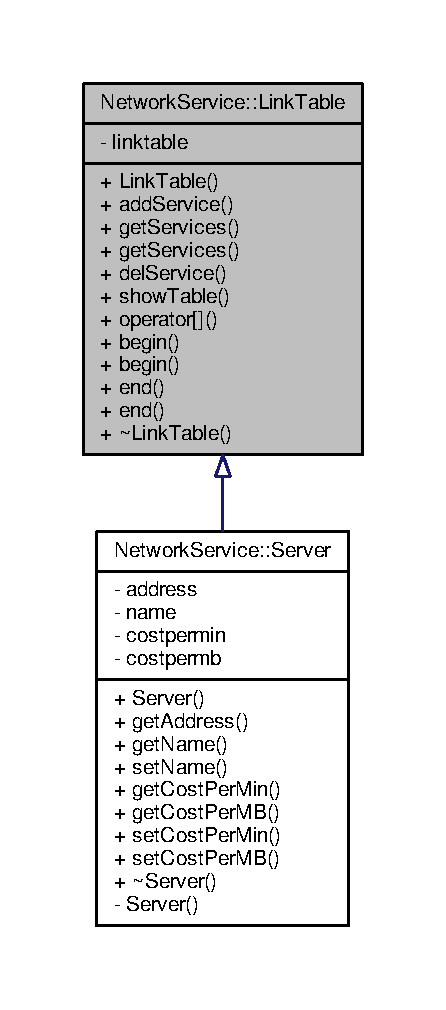
\includegraphics[width=214pt]{class_network_service_1_1_link_table__inherit__graph}
\end{center}
\end{figure}


Граф связей класса Network\+Service\+:\+:Link\+Table\+:\nopagebreak
\begin{figure}[H]
\begin{center}
\leavevmode
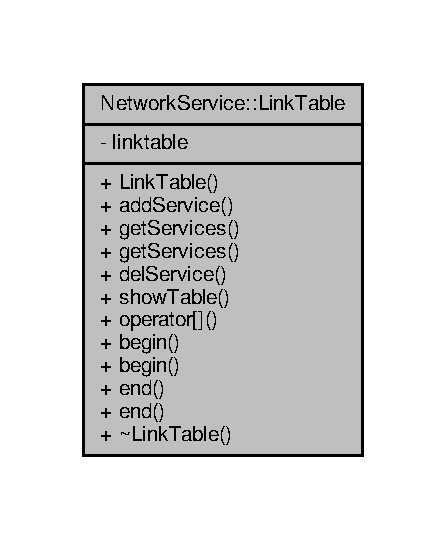
\includegraphics[width=214pt]{class_network_service_1_1_link_table__coll__graph}
\end{center}
\end{figure}
\subsection*{Открытые типы}
\begin{DoxyCompactItemize}
\item 
typedef std\+::pair$<$ \hyperlink{class_network_service_1_1_service_descriptor}{Service\+Descriptor} $\ast$, ulong $>$ \hyperlink{class_network_service_1_1_link_table_a5a0e870806128a79b9947a7ea496fe9e}{index\+T}
\begin{DoxyCompactList}\small\item\em Определение типа для работы итератора \end{DoxyCompactList}\item 
typedef \hyperlink{class_network_service_1_1_my_iterator}{My\+Iterator}$<$ \hyperlink{class_network_service_1_1_link_table}{Link\+Table} $>$ \hyperlink{class_network_service_1_1_link_table_a699ed11fe42478b5269f8c44f7354c77}{Iterator}
\begin{DoxyCompactList}\small\item\em Специализация шаблонного типа \hyperlink{class_network_service_1_1_my_iterator}{My\+Iterator}. \end{DoxyCompactList}\item 
typedef \hyperlink{class_network_service_1_1_my_const_iterator}{My\+Const\+Iterator}$<$ \hyperlink{class_network_service_1_1_link_table}{Link\+Table} $>$ \hyperlink{class_network_service_1_1_link_table_a2414daadb1745ec3039bba9810c8a23d}{Const\+Iterator}
\begin{DoxyCompactList}\small\item\em Специализация шаблонного типа \hyperlink{class_network_service_1_1_my_const_iterator}{My\+Const\+Iterator}. \end{DoxyCompactList}\end{DoxyCompactItemize}
\subsection*{Открытые члены}
\begin{DoxyCompactItemize}
\item 
\hyperlink{class_network_service_1_1_link_table_a3f2e438b8ec892df7cb813a94d74a159}{Link\+Table} ()
\item 
void \hyperlink{class_network_service_1_1_link_table_a31612d870964984c4d6c83208a28684d}{add\+Service} (\hyperlink{class_network_service_1_1_service_descriptor}{Service\+Descriptor} $\ast$sdesc, ulong abonentaddr)
\begin{DoxyCompactList}\small\item\em Добавление записи об оказанной услуге в таблицу \end{DoxyCompactList}\item 
std\+::vector$<$ \hyperlink{class_network_service_1_1_service_descriptor}{Service\+Descriptor} $\ast$ $>$ \hyperlink{class_network_service_1_1_link_table_ac1d3769516f51abd5eb7766d009a54fb}{get\+Services} (ulong abonentaddr) const 
\begin{DoxyCompactList}\small\item\em Получение информации об оказанных услугах для абонента \end{DoxyCompactList}\item 
std\+::vector$<$ \hyperlink{class_network_service_1_1_service_descriptor}{Service\+Descriptor} $\ast$ $>$ \hyperlink{class_network_service_1_1_link_table_a44427b02da77b0478b71ac73ea3e0ef5}{get\+Services} (ulong abonentaddr, \hyperlink{networkservice_8h_ac877dfabb0f4f6a8184aa821b447e81d}{ftimepoint} \&linktime) const 
\begin{DoxyCompactList}\small\item\em Получение информации об оказанных услугах для абонента \end{DoxyCompactList}\item 
void \hyperlink{class_network_service_1_1_link_table_a4aef03eef2e1ed5d60f99075eff7aa96}{del\+Service} (uint index)
\begin{DoxyCompactList}\small\item\em Удаление записи из таблицы \end{DoxyCompactList}\item 
std\+::vector$<$ std\+::string $>$ \hyperlink{class_network_service_1_1_link_table_a5381c7f8fd23c726dd1c89e429f9e8e2}{show\+Table} () const 
\begin{DoxyCompactList}\small\item\em Создать текстовое представление таблицы \end{DoxyCompactList}\item 
\hyperlink{class_network_service_1_1_link_table_a5a0e870806128a79b9947a7ea496fe9e}{index\+T} \& \hyperlink{class_network_service_1_1_link_table_a04e0f13392aff39df1a0847d7667dccd}{operator\mbox{[}$\,$\mbox{]}} (uint index)
\begin{DoxyCompactList}\small\item\em Оператор индексирования \end{DoxyCompactList}\item 
\hyperlink{class_network_service_1_1_link_table_a699ed11fe42478b5269f8c44f7354c77}{Iterator} \hyperlink{class_network_service_1_1_link_table_a72c88d96a4a03fb9dd609df858dac1e6}{begin} ()
\begin{DoxyCompactList}\small\item\em Итератор для первого элемента \end{DoxyCompactList}\item 
\hyperlink{class_network_service_1_1_link_table_a2414daadb1745ec3039bba9810c8a23d}{Const\+Iterator} \hyperlink{class_network_service_1_1_link_table_a0a9a5b10b8a3613ee910d773cff8e272}{begin} () const 
\begin{DoxyCompactList}\small\item\em Константный итератор для первого элемента \end{DoxyCompactList}\item 
\hyperlink{class_network_service_1_1_link_table_a699ed11fe42478b5269f8c44f7354c77}{Iterator} \hyperlink{class_network_service_1_1_link_table_a775b722d34f014953289f7ad069a4567}{end} ()
\begin{DoxyCompactList}\small\item\em Итератор, указывающий на конец таблицы (индекс, равный размеру) \end{DoxyCompactList}\item 
\hyperlink{class_network_service_1_1_link_table_a2414daadb1745ec3039bba9810c8a23d}{Const\+Iterator} \hyperlink{class_network_service_1_1_link_table_a0f21f008e79a83eda18c23c8a416b7c0}{end} () const 
\begin{DoxyCompactList}\small\item\em Константный итератор, указывающий на конец таблицы (индекс, равный размеру) \end{DoxyCompactList}\item 
virtual \hyperlink{class_network_service_1_1_link_table_a4ea276d8834a25c4ed1872f96b324e22}{$\sim$\+Link\+Table} ()
\begin{DoxyCompactList}\small\item\em Деструктор Применяет к указателям на \hyperlink{class_network_service_1_1_service_descriptor}{Service\+Descriptor} оператор delete;. \end{DoxyCompactList}\end{DoxyCompactItemize}
\subsection*{Закрытые данные}
\begin{DoxyCompactItemize}
\item 
std\+::vector$<$ \hyperlink{class_network_service_1_1_link_table_a5a0e870806128a79b9947a7ea496fe9e}{index\+T} $>$ \hyperlink{class_network_service_1_1_link_table_ac5650261ad60d19bb35235b2c4c9a284}{linktable}
\begin{DoxyCompactList}\small\item\em \char`\"{}Таблица связи\char`\"{} \end{DoxyCompactList}\end{DoxyCompactItemize}
\subsection*{Друзья}
\begin{DoxyCompactItemize}
\item 
class \hyperlink{class_network_service_1_1_link_table_a4a2eea20b7b16255ee50c0b05accd544}{My\+Iterator$<$ Link\+Table $>$}
\end{DoxyCompactItemize}


\subsection{Подробное описание}
Класс, реализующий \char`\"{}таблицу связи\char`\"{}. 

\subsection{Определения типов}
\hypertarget{class_network_service_1_1_link_table_a2414daadb1745ec3039bba9810c8a23d}{}\index{Network\+Service\+::\+Link\+Table@{Network\+Service\+::\+Link\+Table}!Const\+Iterator@{Const\+Iterator}}
\index{Const\+Iterator@{Const\+Iterator}!Network\+Service\+::\+Link\+Table@{Network\+Service\+::\+Link\+Table}}
\subsubsection[{Const\+Iterator}]{\setlength{\rightskip}{0pt plus 5cm}typedef {\bf My\+Const\+Iterator}$<${\bf Link\+Table}$>$ {\bf Network\+Service\+::\+Link\+Table\+::\+Const\+Iterator}}\label{class_network_service_1_1_link_table_a2414daadb1745ec3039bba9810c8a23d}


Специализация шаблонного типа \hyperlink{class_network_service_1_1_my_const_iterator}{My\+Const\+Iterator}. 

\hypertarget{class_network_service_1_1_link_table_a5a0e870806128a79b9947a7ea496fe9e}{}\index{Network\+Service\+::\+Link\+Table@{Network\+Service\+::\+Link\+Table}!index\+T@{index\+T}}
\index{index\+T@{index\+T}!Network\+Service\+::\+Link\+Table@{Network\+Service\+::\+Link\+Table}}
\subsubsection[{index\+T}]{\setlength{\rightskip}{0pt plus 5cm}typedef std\+::pair$<${\bf Service\+Descriptor} $\ast$,ulong$>$ {\bf Network\+Service\+::\+Link\+Table\+::index\+T}}\label{class_network_service_1_1_link_table_a5a0e870806128a79b9947a7ea496fe9e}


Определение типа для работы итератора 

\hypertarget{class_network_service_1_1_link_table_a699ed11fe42478b5269f8c44f7354c77}{}\index{Network\+Service\+::\+Link\+Table@{Network\+Service\+::\+Link\+Table}!Iterator@{Iterator}}
\index{Iterator@{Iterator}!Network\+Service\+::\+Link\+Table@{Network\+Service\+::\+Link\+Table}}
\subsubsection[{Iterator}]{\setlength{\rightskip}{0pt plus 5cm}typedef {\bf My\+Iterator}$<${\bf Link\+Table}$>$ {\bf Network\+Service\+::\+Link\+Table\+::\+Iterator}}\label{class_network_service_1_1_link_table_a699ed11fe42478b5269f8c44f7354c77}


Специализация шаблонного типа \hyperlink{class_network_service_1_1_my_iterator}{My\+Iterator}. 



\subsection{Конструктор(ы)}
\hypertarget{class_network_service_1_1_link_table_a3f2e438b8ec892df7cb813a94d74a159}{}\index{Network\+Service\+::\+Link\+Table@{Network\+Service\+::\+Link\+Table}!Link\+Table@{Link\+Table}}
\index{Link\+Table@{Link\+Table}!Network\+Service\+::\+Link\+Table@{Network\+Service\+::\+Link\+Table}}
\subsubsection[{Link\+Table}]{\setlength{\rightskip}{0pt plus 5cm}Link\+Table\+::\+Link\+Table (
\begin{DoxyParamCaption}
{}
\end{DoxyParamCaption}
)}\label{class_network_service_1_1_link_table_a3f2e438b8ec892df7cb813a94d74a159}
\hypertarget{class_network_service_1_1_link_table_a4ea276d8834a25c4ed1872f96b324e22}{}\index{Network\+Service\+::\+Link\+Table@{Network\+Service\+::\+Link\+Table}!````~Link\+Table@{$\sim$\+Link\+Table}}
\index{````~Link\+Table@{$\sim$\+Link\+Table}!Network\+Service\+::\+Link\+Table@{Network\+Service\+::\+Link\+Table}}
\subsubsection[{$\sim$\+Link\+Table}]{\setlength{\rightskip}{0pt plus 5cm}Link\+Table\+::$\sim$\+Link\+Table (
\begin{DoxyParamCaption}
{}
\end{DoxyParamCaption}
)\hspace{0.3cm}{\ttfamily [virtual]}}\label{class_network_service_1_1_link_table_a4ea276d8834a25c4ed1872f96b324e22}


Деструктор Применяет к указателям на \hyperlink{class_network_service_1_1_service_descriptor}{Service\+Descriptor} оператор delete;. 



\subsection{Методы}
\hypertarget{class_network_service_1_1_link_table_a31612d870964984c4d6c83208a28684d}{}\index{Network\+Service\+::\+Link\+Table@{Network\+Service\+::\+Link\+Table}!add\+Service@{add\+Service}}
\index{add\+Service@{add\+Service}!Network\+Service\+::\+Link\+Table@{Network\+Service\+::\+Link\+Table}}
\subsubsection[{add\+Service}]{\setlength{\rightskip}{0pt plus 5cm}void Link\+Table\+::add\+Service (
\begin{DoxyParamCaption}
\item[{{\bf Service\+Descriptor} $\ast$}]{sdesc, }
\item[{ulong}]{abonentaddr}
\end{DoxyParamCaption}
)}\label{class_network_service_1_1_link_table_a31612d870964984c4d6c83208a28684d}


Добавление записи об оказанной услуге в таблицу 


\begin{DoxyParams}{Аргументы}
{\em sdesc} & Указатель на описатель сервиса (полиморфный \hyperlink{class_network_service_1_1_service_descriptor}{Service\+Descriptor}) \\
\hline
{\em abonentaddr} & Адрес абонента, воспользовавшегося услугой \\
\hline
\end{DoxyParams}

\begin{DoxyExceptions}{Исключения}
{\em invalid\+\_\+argument} & если адрес абонента неверен или в качестве указателя передан nullptr \\
\hline
\end{DoxyExceptions}
\hypertarget{class_network_service_1_1_link_table_a72c88d96a4a03fb9dd609df858dac1e6}{}\index{Network\+Service\+::\+Link\+Table@{Network\+Service\+::\+Link\+Table}!begin@{begin}}
\index{begin@{begin}!Network\+Service\+::\+Link\+Table@{Network\+Service\+::\+Link\+Table}}
\subsubsection[{begin}]{\setlength{\rightskip}{0pt plus 5cm}{\bf Link\+Table\+::\+Iterator} Link\+Table\+::begin (
\begin{DoxyParamCaption}
{}
\end{DoxyParamCaption}
)}\label{class_network_service_1_1_link_table_a72c88d96a4a03fb9dd609df858dac1e6}


Итератор для первого элемента 

\begin{DoxyReturn}{Возвращает}
Объект Iterator 
\end{DoxyReturn}
\hypertarget{class_network_service_1_1_link_table_a0a9a5b10b8a3613ee910d773cff8e272}{}\index{Network\+Service\+::\+Link\+Table@{Network\+Service\+::\+Link\+Table}!begin@{begin}}
\index{begin@{begin}!Network\+Service\+::\+Link\+Table@{Network\+Service\+::\+Link\+Table}}
\subsubsection[{begin}]{\setlength{\rightskip}{0pt plus 5cm}{\bf Link\+Table\+::\+Const\+Iterator} Link\+Table\+::begin (
\begin{DoxyParamCaption}
{}
\end{DoxyParamCaption}
) const}\label{class_network_service_1_1_link_table_a0a9a5b10b8a3613ee910d773cff8e272}


Константный итератор для первого элемента 

\begin{DoxyReturn}{Возвращает}
Объект Const\+Iterator 
\end{DoxyReturn}
\hypertarget{class_network_service_1_1_link_table_a4aef03eef2e1ed5d60f99075eff7aa96}{}\index{Network\+Service\+::\+Link\+Table@{Network\+Service\+::\+Link\+Table}!del\+Service@{del\+Service}}
\index{del\+Service@{del\+Service}!Network\+Service\+::\+Link\+Table@{Network\+Service\+::\+Link\+Table}}
\subsubsection[{del\+Service}]{\setlength{\rightskip}{0pt plus 5cm}void Link\+Table\+::del\+Service (
\begin{DoxyParamCaption}
\item[{uint}]{index}
\end{DoxyParamCaption}
)}\label{class_network_service_1_1_link_table_a4aef03eef2e1ed5d60f99075eff7aa96}


Удаление записи из таблицы 


\begin{DoxyParams}{Аргументы}
{\em index} & Индекс записи \\
\hline
\end{DoxyParams}

\begin{DoxyExceptions}{Исключения}
{\em invalid\+\_\+argument} & если индекс больше, чем размер таблицы \\
\hline
\end{DoxyExceptions}
\hypertarget{class_network_service_1_1_link_table_a775b722d34f014953289f7ad069a4567}{}\index{Network\+Service\+::\+Link\+Table@{Network\+Service\+::\+Link\+Table}!end@{end}}
\index{end@{end}!Network\+Service\+::\+Link\+Table@{Network\+Service\+::\+Link\+Table}}
\subsubsection[{end}]{\setlength{\rightskip}{0pt plus 5cm}{\bf Link\+Table\+::\+Iterator} Link\+Table\+::end (
\begin{DoxyParamCaption}
{}
\end{DoxyParamCaption}
)}\label{class_network_service_1_1_link_table_a775b722d34f014953289f7ad069a4567}


Итератор, указывающий на конец таблицы (индекс, равный размеру) 

\begin{DoxyReturn}{Возвращает}
объект Iterator 
\end{DoxyReturn}
\hypertarget{class_network_service_1_1_link_table_a0f21f008e79a83eda18c23c8a416b7c0}{}\index{Network\+Service\+::\+Link\+Table@{Network\+Service\+::\+Link\+Table}!end@{end}}
\index{end@{end}!Network\+Service\+::\+Link\+Table@{Network\+Service\+::\+Link\+Table}}
\subsubsection[{end}]{\setlength{\rightskip}{0pt plus 5cm}{\bf Link\+Table\+::\+Const\+Iterator} Link\+Table\+::end (
\begin{DoxyParamCaption}
{}
\end{DoxyParamCaption}
) const}\label{class_network_service_1_1_link_table_a0f21f008e79a83eda18c23c8a416b7c0}


Константный итератор, указывающий на конец таблицы (индекс, равный размеру) 

\begin{DoxyReturn}{Возвращает}
объект Const\+Iterator 
\end{DoxyReturn}
\hypertarget{class_network_service_1_1_link_table_ac1d3769516f51abd5eb7766d009a54fb}{}\index{Network\+Service\+::\+Link\+Table@{Network\+Service\+::\+Link\+Table}!get\+Services@{get\+Services}}
\index{get\+Services@{get\+Services}!Network\+Service\+::\+Link\+Table@{Network\+Service\+::\+Link\+Table}}
\subsubsection[{get\+Services}]{\setlength{\rightskip}{0pt plus 5cm}std\+::vector$<$ {\bf Service\+Descriptor} $\ast$ $>$ Link\+Table\+::get\+Services (
\begin{DoxyParamCaption}
\item[{ulong}]{abonentaddr}
\end{DoxyParamCaption}
) const}\label{class_network_service_1_1_link_table_ac1d3769516f51abd5eb7766d009a54fb}


Получение информации об оказанных услугах для абонента 


\begin{DoxyParams}{Аргументы}
{\em abonentaddr} & I\+P абонента \\
\hline
\end{DoxyParams}
\begin{DoxyReturn}{Возвращает}
vector из указателей на описатели сервисов (полиморфный \hyperlink{class_network_service_1_1_service_descriptor}{Service\+Descriptor}) 
\end{DoxyReturn}

\begin{DoxyExceptions}{Исключения}
{\em invalid\+\_\+argument} & если I\+P абонента неверен\\
\hline
\end{DoxyExceptions}
Метод обходит всю \char`\"{}таблицу связи\char`\"{} (используется итератор), добавляя нужные описатель к результату \hypertarget{class_network_service_1_1_link_table_a44427b02da77b0478b71ac73ea3e0ef5}{}\index{Network\+Service\+::\+Link\+Table@{Network\+Service\+::\+Link\+Table}!get\+Services@{get\+Services}}
\index{get\+Services@{get\+Services}!Network\+Service\+::\+Link\+Table@{Network\+Service\+::\+Link\+Table}}
\subsubsection[{get\+Services}]{\setlength{\rightskip}{0pt plus 5cm}std\+::vector$<$ {\bf Service\+Descriptor} $\ast$ $>$ Link\+Table\+::get\+Services (
\begin{DoxyParamCaption}
\item[{ulong}]{abonentaddr, }
\item[{{\bf ftimepoint} \&}]{linktime}
\end{DoxyParamCaption}
) const}\label{class_network_service_1_1_link_table_a44427b02da77b0478b71ac73ea3e0ef5}


Получение информации об оказанных услугах для абонента 


\begin{DoxyParams}{Аргументы}
{\em abonentaddr} & I\+P абонента \\
\hline
{\em linktime} & Время оказателей услуги \\
\hline
\end{DoxyParams}
\begin{DoxyReturn}{Возвращает}
vector из указателей на описатели сервисов (полиморфный \hyperlink{class_network_service_1_1_service_descriptor}{Service\+Descriptor}) 
\end{DoxyReturn}

\begin{DoxyExceptions}{Исключения}
{\em invalid\+\_\+argument} & если I\+P абонента неверен\\
\hline
\end{DoxyExceptions}
Метод обходит всю \char`\"{}таблицу связи\char`\"{} (используется итератор), добавляя нужные описатель к результату \hypertarget{class_network_service_1_1_link_table_a04e0f13392aff39df1a0847d7667dccd}{}\index{Network\+Service\+::\+Link\+Table@{Network\+Service\+::\+Link\+Table}!operator\mbox{[}$\,$\mbox{]}@{operator[]}}
\index{operator\mbox{[}$\,$\mbox{]}@{operator[]}!Network\+Service\+::\+Link\+Table@{Network\+Service\+::\+Link\+Table}}
\subsubsection[{operator[]}]{\setlength{\rightskip}{0pt plus 5cm}{\bf Network\+Service\+::\+Link\+Table\+::index\+T} \& Link\+Table\+::operator\mbox{[}$\,$\mbox{]} (
\begin{DoxyParamCaption}
\item[{uint}]{index}
\end{DoxyParamCaption}
)}\label{class_network_service_1_1_link_table_a04e0f13392aff39df1a0847d7667dccd}


Оператор индексирования 


\begin{DoxyParams}{Аргументы}
{\em index} & Индекс \\
\hline
\end{DoxyParams}
\begin{DoxyReturn}{Возвращает}
Ссылка на пару из указателя на описатель сервиса (полиморфный \hyperlink{class_network_service_1_1_service_descriptor}{Service\+Descriptor}) и адреса абонента 
\end{DoxyReturn}

\begin{DoxyExceptions}{Исключения}
{\em invalid\+\_\+argument} & if index is greater then table size \\
\hline
\end{DoxyExceptions}
\hypertarget{class_network_service_1_1_link_table_a5381c7f8fd23c726dd1c89e429f9e8e2}{}\index{Network\+Service\+::\+Link\+Table@{Network\+Service\+::\+Link\+Table}!show\+Table@{show\+Table}}
\index{show\+Table@{show\+Table}!Network\+Service\+::\+Link\+Table@{Network\+Service\+::\+Link\+Table}}
\subsubsection[{show\+Table}]{\setlength{\rightskip}{0pt plus 5cm}std\+::vector$<$ std\+::string $>$ Link\+Table\+::show\+Table (
\begin{DoxyParamCaption}
{}
\end{DoxyParamCaption}
) const}\label{class_network_service_1_1_link_table_a5381c7f8fd23c726dd1c89e429f9e8e2}


Создать текстовое представление таблицы 

\begin{DoxyReturn}{Возвращает}
vector из string с описанием
\end{DoxyReturn}
Метод обходит всю \char`\"{}таблицу связи\char`\"{} (используется итератор), создавая для каждого элемента описывающюю его строку и добавляя её к результату 

\subsection{Документация по друзьям класса и функциям, относящимся к классу}
\hypertarget{class_network_service_1_1_link_table_a4a2eea20b7b16255ee50c0b05accd544}{}\index{Network\+Service\+::\+Link\+Table@{Network\+Service\+::\+Link\+Table}!My\+Iterator$<$ Link\+Table $>$@{My\+Iterator$<$ Link\+Table $>$}}
\index{My\+Iterator$<$ Link\+Table $>$@{My\+Iterator$<$ Link\+Table $>$}!Network\+Service\+::\+Link\+Table@{Network\+Service\+::\+Link\+Table}}
\subsubsection[{My\+Iterator$<$ Link\+Table $>$}]{\setlength{\rightskip}{0pt plus 5cm}friend class {\bf My\+Iterator}$<$ {\bf Link\+Table} $>$\hspace{0.3cm}{\ttfamily [friend]}}\label{class_network_service_1_1_link_table_a4a2eea20b7b16255ee50c0b05accd544}


\subsection{Данные класса}
\hypertarget{class_network_service_1_1_link_table_ac5650261ad60d19bb35235b2c4c9a284}{}\index{Network\+Service\+::\+Link\+Table@{Network\+Service\+::\+Link\+Table}!linktable@{linktable}}
\index{linktable@{linktable}!Network\+Service\+::\+Link\+Table@{Network\+Service\+::\+Link\+Table}}
\subsubsection[{linktable}]{\setlength{\rightskip}{0pt plus 5cm}std\+::vector$<${\bf index\+T}$>$ Network\+Service\+::\+Link\+Table\+::linktable\hspace{0.3cm}{\ttfamily [private]}}\label{class_network_service_1_1_link_table_ac5650261ad60d19bb35235b2c4c9a284}


\char`\"{}Таблица связи\char`\"{} 



Объявления и описания членов классов находятся в файлах\+:\begin{DoxyCompactItemize}
\item 
Network\+Service\+Lib/\hyperlink{linktable_8h}{linktable.\+h}\item 
Network\+Service\+Lib/\hyperlink{linktable_8cpp}{linktable.\+cpp}\end{DoxyCompactItemize}

\hypertarget{class_network_service_1_1_my_const_iterator}{}\section{Шаблон класса Network\+Service\+:\+:My\+Const\+Iterator$<$ T $>$}
\label{class_network_service_1_1_my_const_iterator}\index{Network\+Service\+::\+My\+Const\+Iterator$<$ T $>$@{Network\+Service\+::\+My\+Const\+Iterator$<$ T $>$}}


Шаблонный класс итератора  




{\ttfamily \#include $<$myiterator.\+h$>$}



Граф наследования\+:Network\+Service\+:\+:My\+Const\+Iterator$<$ T $>$\+:\nopagebreak
\begin{figure}[H]
\begin{center}
\leavevmode
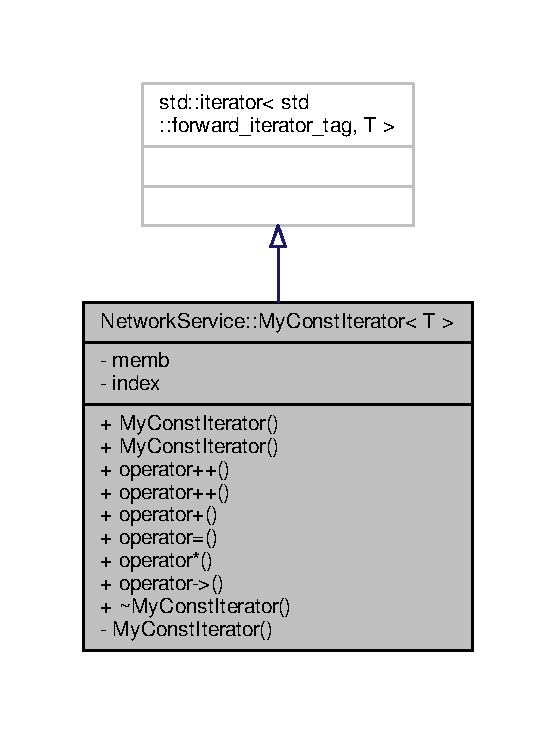
\includegraphics[width=267pt]{class_network_service_1_1_my_const_iterator__inherit__graph}
\end{center}
\end{figure}


Граф связей класса Network\+Service\+:\+:My\+Const\+Iterator$<$ T $>$\+:\nopagebreak
\begin{figure}[H]
\begin{center}
\leavevmode
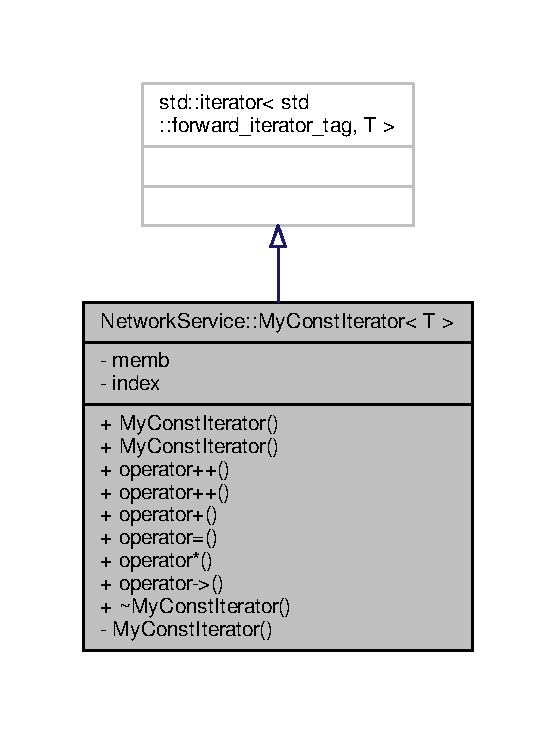
\includegraphics[width=267pt]{class_network_service_1_1_my_const_iterator__coll__graph}
\end{center}
\end{figure}
\subsection*{Открытые члены}
\begin{DoxyCompactItemize}
\item 
\hyperlink{class_network_service_1_1_my_const_iterator_a7e183160817f8b9dadf9d4a857d9ccaf}{My\+Const\+Iterator} (const T $\ast$nmemb, uint idx)
\begin{DoxyCompactList}\small\item\em Инициализирующий конструктор \end{DoxyCompactList}\item 
\hyperlink{class_network_service_1_1_my_const_iterator_a2af24e77940dce68ffeac3dc5d502755}{My\+Const\+Iterator} (const \hyperlink{class_network_service_1_1_my_const_iterator}{My\+Const\+Iterator} \&it)
\begin{DoxyCompactList}\small\item\em Копирующий конструктор \end{DoxyCompactList}\item 
\hyperlink{class_network_service_1_1_my_const_iterator}{My\+Const\+Iterator} \& \hyperlink{class_network_service_1_1_my_const_iterator_ab4f583f1037994c6cb7c8900d08aad75}{operator++} ()
\begin{DoxyCompactList}\small\item\em Увеличение индекса на 1 (постфиксный оператор) \end{DoxyCompactList}\item 
\hyperlink{class_network_service_1_1_my_const_iterator}{My\+Const\+Iterator} \hyperlink{class_network_service_1_1_my_const_iterator_ae5f5bac3cb72a1dd8e94e162b38d0cdd}{operator++} (int)
\begin{DoxyCompactList}\small\item\em Увеличение индекса на 1 (префиксный оператор) \end{DoxyCompactList}\item 
\hyperlink{class_network_service_1_1_my_const_iterator}{My\+Const\+Iterator} \hyperlink{class_network_service_1_1_my_const_iterator_a0c18a1dd9c0b66ed30f0a81046ffd7c1}{operator+} (int toadd)
\begin{DoxyCompactList}\small\item\em Получение итератора добавлением к индексу \end{DoxyCompactList}\item 
\hyperlink{class_network_service_1_1_my_const_iterator}{My\+Const\+Iterator} \& \hyperlink{class_network_service_1_1_my_const_iterator_a53aad52b888c357044143021be3f3de4}{operator=} (const \hyperlink{class_network_service_1_1_my_const_iterator}{My\+Const\+Iterator} \&it)
\begin{DoxyCompactList}\small\item\em Копирующий оператор присваивания \end{DoxyCompactList}\item 
const T\+::index\+T \& \hyperlink{class_network_service_1_1_my_const_iterator_a7e881c108297cb10d072347e9ff86300}{operator$\ast$} ()
\begin{DoxyCompactList}\small\item\em Разыменовывание (обращение к элементу итерируемого объекта по индексу) \end{DoxyCompactList}\item 
const T\+::index\+T $\ast$ \hyperlink{class_network_service_1_1_my_const_iterator_a77f6dccb9a4a298307b8ba81dcaafeb6}{operator-\/$>$} ()
\begin{DoxyCompactList}\small\item\em Доступ к членам объекта, создающего коллекцию \end{DoxyCompactList}\item 
virtual \hyperlink{class_network_service_1_1_my_const_iterator_a3d169b0e5975d614272a0c8a3573cc25}{$\sim$\+My\+Const\+Iterator} ()
\end{DoxyCompactItemize}
\subsection*{Закрытые члены}
\begin{DoxyCompactItemize}
\item 
\hyperlink{class_network_service_1_1_my_const_iterator_ab1acfcd83f296465c285a336e8fb6e69}{My\+Const\+Iterator} ()
\begin{DoxyCompactList}\small\item\em Отключение создания через пустой конструктор для предотвращения обращения к nullptr. \end{DoxyCompactList}\end{DoxyCompactItemize}
\subsection*{Закрытые данные}
\begin{DoxyCompactItemize}
\item 
const T $\ast$ \hyperlink{class_network_service_1_1_my_const_iterator_ac9879e15103086204afa1af2aa6341a5}{memb}
\begin{DoxyCompactList}\small\item\em Константный указатель на итерируемый объект \end{DoxyCompactList}\item 
uint \hyperlink{class_network_service_1_1_my_const_iterator_a9350ef04e3633db10f91f6662d1df1a4}{index}
\begin{DoxyCompactList}\small\item\em Индекс текущего элемента \end{DoxyCompactList}\end{DoxyCompactItemize}
\subsection*{Друзья}
\begin{DoxyCompactItemize}
\item 
bool \hyperlink{class_network_service_1_1_my_const_iterator_ac56e784eab6a4e2ec2009df237d19f4e}{operator==} (const \hyperlink{class_network_service_1_1_my_const_iterator}{My\+Const\+Iterator} \&lv, const \hyperlink{class_network_service_1_1_my_const_iterator}{My\+Const\+Iterator} \&rv)
\begin{DoxyCompactList}\small\item\em Равенство двух итераторов \end{DoxyCompactList}\item 
bool \hyperlink{class_network_service_1_1_my_const_iterator_a133b066e84ae10176ec5a109ce55f0e0}{operator!=} (const \hyperlink{class_network_service_1_1_my_const_iterator}{My\+Const\+Iterator} \&lv, const \hyperlink{class_network_service_1_1_my_const_iterator}{My\+Const\+Iterator} \&rv)
\begin{DoxyCompactList}\small\item\em Неравенство двух итераторов \end{DoxyCompactList}\end{DoxyCompactItemize}


\subsection{Подробное описание}
\subsubsection*{template$<$class T$>$class Network\+Service\+::\+My\+Const\+Iterator$<$ T $>$}

Шаблонный класс итератора 

Первый параметр шаблона -\/ класс, к которому прикрепляется итератор Для корректной работы требуется следующее\+:
\begin{DoxyItemize}
\item Переопределенный тип index\+T (тип, возвращаемый оператором \mbox{[}\mbox{]})
\item Перегруженный оператор \mbox{[}\mbox{]} Отличается от обычного итератора тем, что не позволяет изменять значение элемента, на который он указывает 
\end{DoxyItemize}

\subsection{Конструктор(ы)}
\hypertarget{class_network_service_1_1_my_const_iterator_ab1acfcd83f296465c285a336e8fb6e69}{}\index{Network\+Service\+::\+My\+Const\+Iterator@{Network\+Service\+::\+My\+Const\+Iterator}!My\+Const\+Iterator@{My\+Const\+Iterator}}
\index{My\+Const\+Iterator@{My\+Const\+Iterator}!Network\+Service\+::\+My\+Const\+Iterator@{Network\+Service\+::\+My\+Const\+Iterator}}
\subsubsection[{My\+Const\+Iterator}]{\setlength{\rightskip}{0pt plus 5cm}template$<$class T$>$ {\bf Network\+Service\+::\+My\+Const\+Iterator}$<$ T $>$\+::{\bf My\+Const\+Iterator} (
\begin{DoxyParamCaption}
{}
\end{DoxyParamCaption}
)\hspace{0.3cm}{\ttfamily [private]}}\label{class_network_service_1_1_my_const_iterator_ab1acfcd83f296465c285a336e8fb6e69}


Отключение создания через пустой конструктор для предотвращения обращения к nullptr. 

\hypertarget{class_network_service_1_1_my_const_iterator_a7e183160817f8b9dadf9d4a857d9ccaf}{}\index{Network\+Service\+::\+My\+Const\+Iterator@{Network\+Service\+::\+My\+Const\+Iterator}!My\+Const\+Iterator@{My\+Const\+Iterator}}
\index{My\+Const\+Iterator@{My\+Const\+Iterator}!Network\+Service\+::\+My\+Const\+Iterator@{Network\+Service\+::\+My\+Const\+Iterator}}
\subsubsection[{My\+Const\+Iterator}]{\setlength{\rightskip}{0pt plus 5cm}template$<$class T$>$ {\bf Network\+Service\+::\+My\+Const\+Iterator}$<$ T $>$\+::{\bf My\+Const\+Iterator} (
\begin{DoxyParamCaption}
\item[{const T $\ast$}]{nmemb, }
\item[{uint}]{idx}
\end{DoxyParamCaption}
)\hspace{0.3cm}{\ttfamily [inline]}, {\ttfamily [explicit]}}\label{class_network_service_1_1_my_const_iterator_a7e183160817f8b9dadf9d4a857d9ccaf}


Инициализирующий конструктор 


\begin{DoxyParams}{Аргументы}
{\em nmemb} & Указатель на итерируемый объект \\
\hline
{\em idx} & Индекс \\
\hline
\end{DoxyParams}

\begin{DoxyExceptions}{Исключения}
{\em invalid\+\_\+argument,если} & в качетсве указателя передан nullptr \\
\hline
\end{DoxyExceptions}
\hypertarget{class_network_service_1_1_my_const_iterator_a2af24e77940dce68ffeac3dc5d502755}{}\index{Network\+Service\+::\+My\+Const\+Iterator@{Network\+Service\+::\+My\+Const\+Iterator}!My\+Const\+Iterator@{My\+Const\+Iterator}}
\index{My\+Const\+Iterator@{My\+Const\+Iterator}!Network\+Service\+::\+My\+Const\+Iterator@{Network\+Service\+::\+My\+Const\+Iterator}}
\subsubsection[{My\+Const\+Iterator}]{\setlength{\rightskip}{0pt plus 5cm}template$<$class T$>$ {\bf Network\+Service\+::\+My\+Const\+Iterator}$<$ T $>$\+::{\bf My\+Const\+Iterator} (
\begin{DoxyParamCaption}
\item[{const {\bf My\+Const\+Iterator}$<$ T $>$ \&}]{it}
\end{DoxyParamCaption}
)\hspace{0.3cm}{\ttfamily [inline]}}\label{class_network_service_1_1_my_const_iterator_a2af24e77940dce68ffeac3dc5d502755}


Копирующий конструктор 


\begin{DoxyParams}{Аргументы}
{\em it} & Исходный объект \\
\hline
\end{DoxyParams}
\hypertarget{class_network_service_1_1_my_const_iterator_a3d169b0e5975d614272a0c8a3573cc25}{}\index{Network\+Service\+::\+My\+Const\+Iterator@{Network\+Service\+::\+My\+Const\+Iterator}!````~My\+Const\+Iterator@{$\sim$\+My\+Const\+Iterator}}
\index{````~My\+Const\+Iterator@{$\sim$\+My\+Const\+Iterator}!Network\+Service\+::\+My\+Const\+Iterator@{Network\+Service\+::\+My\+Const\+Iterator}}
\subsubsection[{$\sim$\+My\+Const\+Iterator}]{\setlength{\rightskip}{0pt plus 5cm}template$<$class T$>$ virtual {\bf Network\+Service\+::\+My\+Const\+Iterator}$<$ T $>$\+::$\sim${\bf My\+Const\+Iterator} (
\begin{DoxyParamCaption}
{}
\end{DoxyParamCaption}
)\hspace{0.3cm}{\ttfamily [virtual]}}\label{class_network_service_1_1_my_const_iterator_a3d169b0e5975d614272a0c8a3573cc25}


\subsection{Методы}
\hypertarget{class_network_service_1_1_my_const_iterator_a7e881c108297cb10d072347e9ff86300}{}\index{Network\+Service\+::\+My\+Const\+Iterator@{Network\+Service\+::\+My\+Const\+Iterator}!operator$\ast$@{operator$\ast$}}
\index{operator$\ast$@{operator$\ast$}!Network\+Service\+::\+My\+Const\+Iterator@{Network\+Service\+::\+My\+Const\+Iterator}}
\subsubsection[{operator$\ast$}]{\setlength{\rightskip}{0pt plus 5cm}template$<$class T$>$ const T\+::index\+T\& {\bf Network\+Service\+::\+My\+Const\+Iterator}$<$ T $>$\+::operator$\ast$ (
\begin{DoxyParamCaption}
{}
\end{DoxyParamCaption}
)\hspace{0.3cm}{\ttfamily [inline]}}\label{class_network_service_1_1_my_const_iterator_a7e881c108297cb10d072347e9ff86300}


Разыменовывание (обращение к элементу итерируемого объекта по индексу) 

\begin{DoxyReturn}{Возвращает}
Константная ссылка на объект
\end{DoxyReturn}
Разыменовывание с использованием перегруженного оператора \mbox{[}\mbox{]} с последующим динамическим приведением типа \hypertarget{class_network_service_1_1_my_const_iterator_a0c18a1dd9c0b66ed30f0a81046ffd7c1}{}\index{Network\+Service\+::\+My\+Const\+Iterator@{Network\+Service\+::\+My\+Const\+Iterator}!operator+@{operator+}}
\index{operator+@{operator+}!Network\+Service\+::\+My\+Const\+Iterator@{Network\+Service\+::\+My\+Const\+Iterator}}
\subsubsection[{operator+}]{\setlength{\rightskip}{0pt plus 5cm}template$<$class T$>$ {\bf My\+Const\+Iterator} {\bf Network\+Service\+::\+My\+Const\+Iterator}$<$ T $>$\+::operator+ (
\begin{DoxyParamCaption}
\item[{int}]{toadd}
\end{DoxyParamCaption}
)\hspace{0.3cm}{\ttfamily [inline]}}\label{class_network_service_1_1_my_const_iterator_a0c18a1dd9c0b66ed30f0a81046ffd7c1}


Получение итератора добавлением к индексу 


\begin{DoxyParams}{Аргументы}
{\em toadd} & Число, добавляемое к текущему индексу \\
\hline
\end{DoxyParams}
\begin{DoxyReturn}{Возвращает}
Новый объект итератора с измененным индексом 
\end{DoxyReturn}
\hypertarget{class_network_service_1_1_my_const_iterator_ab4f583f1037994c6cb7c8900d08aad75}{}\index{Network\+Service\+::\+My\+Const\+Iterator@{Network\+Service\+::\+My\+Const\+Iterator}!operator++@{operator++}}
\index{operator++@{operator++}!Network\+Service\+::\+My\+Const\+Iterator@{Network\+Service\+::\+My\+Const\+Iterator}}
\subsubsection[{operator++}]{\setlength{\rightskip}{0pt plus 5cm}template$<$class T$>$ {\bf My\+Const\+Iterator}\& {\bf Network\+Service\+::\+My\+Const\+Iterator}$<$ T $>$\+::operator++ (
\begin{DoxyParamCaption}
{}
\end{DoxyParamCaption}
)\hspace{0.3cm}{\ttfamily [inline]}}\label{class_network_service_1_1_my_const_iterator_ab4f583f1037994c6cb7c8900d08aad75}


Увеличение индекса на 1 (постфиксный оператор) 

\hypertarget{class_network_service_1_1_my_const_iterator_ae5f5bac3cb72a1dd8e94e162b38d0cdd}{}\index{Network\+Service\+::\+My\+Const\+Iterator@{Network\+Service\+::\+My\+Const\+Iterator}!operator++@{operator++}}
\index{operator++@{operator++}!Network\+Service\+::\+My\+Const\+Iterator@{Network\+Service\+::\+My\+Const\+Iterator}}
\subsubsection[{operator++}]{\setlength{\rightskip}{0pt plus 5cm}template$<$class T$>$ {\bf My\+Const\+Iterator} {\bf Network\+Service\+::\+My\+Const\+Iterator}$<$ T $>$\+::operator++ (
\begin{DoxyParamCaption}
\item[{int}]{}
\end{DoxyParamCaption}
)\hspace{0.3cm}{\ttfamily [inline]}}\label{class_network_service_1_1_my_const_iterator_ae5f5bac3cb72a1dd8e94e162b38d0cdd}


Увеличение индекса на 1 (префиксный оператор) 

Используется создание временного объекта итератора \hypertarget{class_network_service_1_1_my_const_iterator_a77f6dccb9a4a298307b8ba81dcaafeb6}{}\index{Network\+Service\+::\+My\+Const\+Iterator@{Network\+Service\+::\+My\+Const\+Iterator}!operator-\/$>$@{operator-\/$>$}}
\index{operator-\/$>$@{operator-\/$>$}!Network\+Service\+::\+My\+Const\+Iterator@{Network\+Service\+::\+My\+Const\+Iterator}}
\subsubsection[{operator-\/$>$}]{\setlength{\rightskip}{0pt plus 5cm}template$<$class T$>$ const T\+::index\+T$\ast$ {\bf Network\+Service\+::\+My\+Const\+Iterator}$<$ T $>$\+::operator-\/$>$ (
\begin{DoxyParamCaption}
{}
\end{DoxyParamCaption}
)\hspace{0.3cm}{\ttfamily [inline]}}\label{class_network_service_1_1_my_const_iterator_a77f6dccb9a4a298307b8ba81dcaafeb6}


Доступ к членам объекта, создающего коллекцию 

\begin{DoxyReturn}{Возвращает}
Константный указатель на объект, создающий коллекцию
\end{DoxyReturn}
Получение указателя на элемент коллекции с помощью перегруженного оператора \mbox{[}\mbox{]} с последующим динамическим приведением типа \hypertarget{class_network_service_1_1_my_const_iterator_a53aad52b888c357044143021be3f3de4}{}\index{Network\+Service\+::\+My\+Const\+Iterator@{Network\+Service\+::\+My\+Const\+Iterator}!operator=@{operator=}}
\index{operator=@{operator=}!Network\+Service\+::\+My\+Const\+Iterator@{Network\+Service\+::\+My\+Const\+Iterator}}
\subsubsection[{operator=}]{\setlength{\rightskip}{0pt plus 5cm}template$<$class T$>$ {\bf My\+Const\+Iterator}\& {\bf Network\+Service\+::\+My\+Const\+Iterator}$<$ T $>$\+::operator= (
\begin{DoxyParamCaption}
\item[{const {\bf My\+Const\+Iterator}$<$ T $>$ \&}]{it}
\end{DoxyParamCaption}
)\hspace{0.3cm}{\ttfamily [inline]}}\label{class_network_service_1_1_my_const_iterator_a53aad52b888c357044143021be3f3de4}


Копирующий оператор присваивания 

Оператор присваивания, копирующий объект итератора. Корректно обрабатывает присваивание самому себе 

\subsection{Документация по друзьям класса и функциям, относящимся к классу}
\hypertarget{class_network_service_1_1_my_const_iterator_a133b066e84ae10176ec5a109ce55f0e0}{}\index{Network\+Service\+::\+My\+Const\+Iterator@{Network\+Service\+::\+My\+Const\+Iterator}!operator"!=@{operator"!=}}
\index{operator"!=@{operator"!=}!Network\+Service\+::\+My\+Const\+Iterator@{Network\+Service\+::\+My\+Const\+Iterator}}
\subsubsection[{operator"!=}]{\setlength{\rightskip}{0pt plus 5cm}template$<$class T$>$ bool operator!= (
\begin{DoxyParamCaption}
\item[{const {\bf My\+Const\+Iterator}$<$ T $>$ \&}]{lv, }
\item[{const {\bf My\+Const\+Iterator}$<$ T $>$ \&}]{rv}
\end{DoxyParamCaption}
)\hspace{0.3cm}{\ttfamily [friend]}}\label{class_network_service_1_1_my_const_iterator_a133b066e84ae10176ec5a109ce55f0e0}


Неравенство двух итераторов 


\begin{DoxyParams}{Аргументы}
{\em lv} & Итератор слева от знака == \\
\hline
{\em rv} & Итератор справа от знака == \\
\hline
\end{DoxyParams}
\begin{DoxyReturn}{Возвращает}
true, если итераторы неравны, false в противном случае
\end{DoxyReturn}
Обращение результата оператора == \hypertarget{class_network_service_1_1_my_const_iterator_ac56e784eab6a4e2ec2009df237d19f4e}{}\index{Network\+Service\+::\+My\+Const\+Iterator@{Network\+Service\+::\+My\+Const\+Iterator}!operator==@{operator==}}
\index{operator==@{operator==}!Network\+Service\+::\+My\+Const\+Iterator@{Network\+Service\+::\+My\+Const\+Iterator}}
\subsubsection[{operator==}]{\setlength{\rightskip}{0pt plus 5cm}template$<$class T$>$ bool operator== (
\begin{DoxyParamCaption}
\item[{const {\bf My\+Const\+Iterator}$<$ T $>$ \&}]{lv, }
\item[{const {\bf My\+Const\+Iterator}$<$ T $>$ \&}]{rv}
\end{DoxyParamCaption}
)\hspace{0.3cm}{\ttfamily [friend]}}\label{class_network_service_1_1_my_const_iterator_ac56e784eab6a4e2ec2009df237d19f4e}


Равенство двух итераторов 


\begin{DoxyParams}{Аргументы}
{\em lv} & Итератор слева от знака == \\
\hline
{\em rv} & Итератор справа от знака == \\
\hline
\end{DoxyParams}
\begin{DoxyReturn}{Возвращает}
true, если итераторы равны, false в противном случае
\end{DoxyReturn}
Итераторы считаются равными, если у них совпадают указатели на итерируемый объект и индексы 

\subsection{Данные класса}
\hypertarget{class_network_service_1_1_my_const_iterator_a9350ef04e3633db10f91f6662d1df1a4}{}\index{Network\+Service\+::\+My\+Const\+Iterator@{Network\+Service\+::\+My\+Const\+Iterator}!index@{index}}
\index{index@{index}!Network\+Service\+::\+My\+Const\+Iterator@{Network\+Service\+::\+My\+Const\+Iterator}}
\subsubsection[{index}]{\setlength{\rightskip}{0pt plus 5cm}template$<$class T$>$ uint {\bf Network\+Service\+::\+My\+Const\+Iterator}$<$ T $>$\+::index\hspace{0.3cm}{\ttfamily [private]}}\label{class_network_service_1_1_my_const_iterator_a9350ef04e3633db10f91f6662d1df1a4}


Индекс текущего элемента 

\hypertarget{class_network_service_1_1_my_const_iterator_ac9879e15103086204afa1af2aa6341a5}{}\index{Network\+Service\+::\+My\+Const\+Iterator@{Network\+Service\+::\+My\+Const\+Iterator}!memb@{memb}}
\index{memb@{memb}!Network\+Service\+::\+My\+Const\+Iterator@{Network\+Service\+::\+My\+Const\+Iterator}}
\subsubsection[{memb}]{\setlength{\rightskip}{0pt plus 5cm}template$<$class T$>$ const T$\ast$ {\bf Network\+Service\+::\+My\+Const\+Iterator}$<$ T $>$\+::memb\hspace{0.3cm}{\ttfamily [private]}}\label{class_network_service_1_1_my_const_iterator_ac9879e15103086204afa1af2aa6341a5}


Константный указатель на итерируемый объект 



Объявления и описания членов класса находятся в файле\+:\begin{DoxyCompactItemize}
\item 
Network\+Service\+Lib/\hyperlink{myiterator_8h}{myiterator.\+h}\end{DoxyCompactItemize}

\hypertarget{class_network_service_1_1_my_iterator}{}\section{Шаблон класса Network\+Service\+:\+:My\+Iterator$<$ T $>$}
\label{class_network_service_1_1_my_iterator}\index{Network\+Service\+::\+My\+Iterator$<$ T $>$@{Network\+Service\+::\+My\+Iterator$<$ T $>$}}


Шаблонный класс итератора  




{\ttfamily \#include $<$myiterator.\+h$>$}



Граф наследования\+:Network\+Service\+:\+:My\+Iterator$<$ T $>$\+:\nopagebreak
\begin{figure}[H]
\begin{center}
\leavevmode
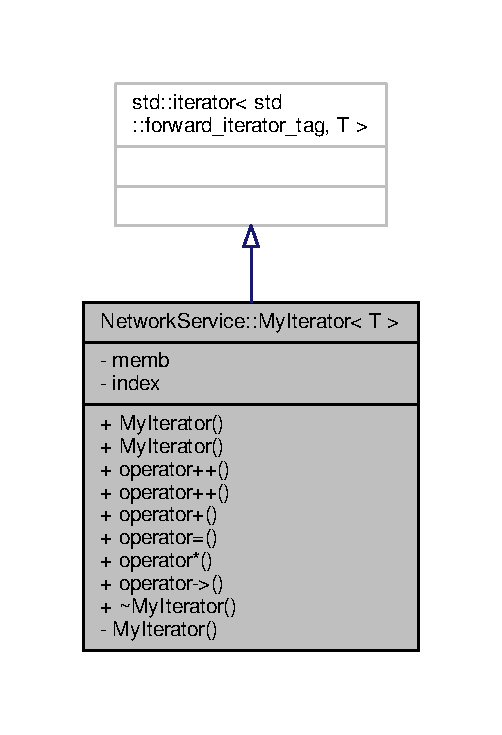
\includegraphics[width=241pt]{class_network_service_1_1_my_iterator__inherit__graph}
\end{center}
\end{figure}


Граф связей класса Network\+Service\+:\+:My\+Iterator$<$ T $>$\+:\nopagebreak
\begin{figure}[H]
\begin{center}
\leavevmode
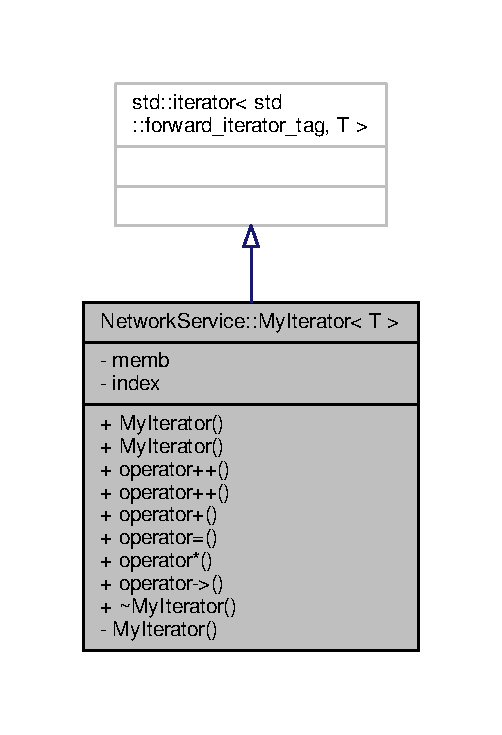
\includegraphics[width=241pt]{class_network_service_1_1_my_iterator__coll__graph}
\end{center}
\end{figure}
\subsection*{Открытые члены}
\begin{DoxyCompactItemize}
\item 
\hyperlink{class_network_service_1_1_my_iterator_a0d0c83ad52ec18d29f026ead351562e4}{My\+Iterator} (T $\ast$nmemb, uint idx)
\begin{DoxyCompactList}\small\item\em Инициализирующий конструктор \end{DoxyCompactList}\item 
\hyperlink{class_network_service_1_1_my_iterator_afaab5f5b3b934271e81341e22946159d}{My\+Iterator} (const \hyperlink{class_network_service_1_1_my_iterator}{My\+Iterator} \&it)
\begin{DoxyCompactList}\small\item\em Копирующий конструктор \end{DoxyCompactList}\item 
\hyperlink{class_network_service_1_1_my_iterator}{My\+Iterator} \& \hyperlink{class_network_service_1_1_my_iterator_ae71706eb096475404afa566e8355b439}{operator++} ()
\begin{DoxyCompactList}\small\item\em Увеличение индекса на 1 (постфиксный оператор) \end{DoxyCompactList}\item 
\hyperlink{class_network_service_1_1_my_iterator}{My\+Iterator} \hyperlink{class_network_service_1_1_my_iterator_a3f7fb28a18f0838385163b8bf3ea96d8}{operator++} (int)
\begin{DoxyCompactList}\small\item\em Увеличение индекса на 1 (префиксный оператор) Используется создание временного объекта итератора \end{DoxyCompactList}\item 
\hyperlink{class_network_service_1_1_my_iterator}{My\+Iterator} \hyperlink{class_network_service_1_1_my_iterator_a86a2b003c3396f38b06abecda8b7c8da}{operator+} (int toadd)
\begin{DoxyCompactList}\small\item\em Получение итератора добавлением к индексу \end{DoxyCompactList}\item 
\hyperlink{class_network_service_1_1_my_iterator}{My\+Iterator} \& \hyperlink{class_network_service_1_1_my_iterator_abbcd1a24586f40134de65d2d914e17db}{operator=} (const \hyperlink{class_network_service_1_1_my_iterator}{My\+Iterator} \&it)
\begin{DoxyCompactList}\small\item\em Копирующий оператор присваивания \end{DoxyCompactList}\item 
T\+::index\+T \& \hyperlink{class_network_service_1_1_my_iterator_ad6babde77410209a9972b5d2d5a29078}{operator$\ast$} ()
\begin{DoxyCompactList}\small\item\em Разыменовывание (обращение к элементу итерируемого объекта по индексу) \end{DoxyCompactList}\item 
T\+::index\+T $\ast$ \hyperlink{class_network_service_1_1_my_iterator_a425cc9c1dba308bb467d4d3122fb7457}{operator-\/$>$} ()
\begin{DoxyCompactList}\small\item\em Доступ к членам объекта, создающего коллекцию \end{DoxyCompactList}\item 
virtual \hyperlink{class_network_service_1_1_my_iterator_a2c2f5449fafddaf6f8a3557265f0d2d9}{$\sim$\+My\+Iterator} ()
\end{DoxyCompactItemize}
\subsection*{Закрытые члены}
\begin{DoxyCompactItemize}
\item 
\hyperlink{class_network_service_1_1_my_iterator_afdc20f191ceb30ab06cd7f10d4a6b699}{My\+Iterator} ()
\begin{DoxyCompactList}\small\item\em Отключение создания через пустой конструктор для предотвращения обращения к nullptr. \end{DoxyCompactList}\end{DoxyCompactItemize}
\subsection*{Закрытые данные}
\begin{DoxyCompactItemize}
\item 
T $\ast$ \hyperlink{class_network_service_1_1_my_iterator_a72858d4e9cc8cc8154f9e028ffa09aa7}{memb}
\begin{DoxyCompactList}\small\item\em Указатель на итерируемый объект \end{DoxyCompactList}\item 
uint \hyperlink{class_network_service_1_1_my_iterator_af3988a37b15d4fc081c55b2c21a93ad3}{index}
\begin{DoxyCompactList}\small\item\em Индекс текущего элемента \end{DoxyCompactList}\end{DoxyCompactItemize}
\subsection*{Друзья}
\begin{DoxyCompactItemize}
\item 
bool \hyperlink{class_network_service_1_1_my_iterator_a44acb87c982f4dd4b401b1e46e7b93b7}{operator==} (\hyperlink{class_network_service_1_1_my_iterator}{My\+Iterator} \&lv, \hyperlink{class_network_service_1_1_my_iterator}{My\+Iterator} \&rv)
\begin{DoxyCompactList}\small\item\em Равенство двух итераторов \end{DoxyCompactList}\item 
bool \hyperlink{class_network_service_1_1_my_iterator_a3ef5b0b89d2266aa10cb593e6b2d1255}{operator!=} (\hyperlink{class_network_service_1_1_my_iterator}{My\+Iterator} \&lv, \hyperlink{class_network_service_1_1_my_iterator}{My\+Iterator} \&rv)
\begin{DoxyCompactList}\small\item\em Неравенство двух итераторов \end{DoxyCompactList}\end{DoxyCompactItemize}


\subsection{Подробное описание}
\subsubsection*{template$<$class T$>$class Network\+Service\+::\+My\+Iterator$<$ T $>$}

Шаблонный класс итератора 

Первый параметр шаблона -\/ класс, к которому прикрепляется итератор Для корректной работы требуется следующее\+:
\begin{DoxyItemize}
\item Переопределенный тип index\+T (тип, возвращаемый оператором \mbox{[}\mbox{]})
\item Перегруженный оператор \mbox{[}\mbox{]} 
\end{DoxyItemize}

\subsection{Конструктор(ы)}
\hypertarget{class_network_service_1_1_my_iterator_afdc20f191ceb30ab06cd7f10d4a6b699}{}\index{Network\+Service\+::\+My\+Iterator@{Network\+Service\+::\+My\+Iterator}!My\+Iterator@{My\+Iterator}}
\index{My\+Iterator@{My\+Iterator}!Network\+Service\+::\+My\+Iterator@{Network\+Service\+::\+My\+Iterator}}
\subsubsection[{My\+Iterator}]{\setlength{\rightskip}{0pt plus 5cm}template$<$class T$>$ {\bf Network\+Service\+::\+My\+Iterator}$<$ T $>$\+::{\bf My\+Iterator} (
\begin{DoxyParamCaption}
{}
\end{DoxyParamCaption}
)\hspace{0.3cm}{\ttfamily [private]}}\label{class_network_service_1_1_my_iterator_afdc20f191ceb30ab06cd7f10d4a6b699}


Отключение создания через пустой конструктор для предотвращения обращения к nullptr. 

\hypertarget{class_network_service_1_1_my_iterator_a0d0c83ad52ec18d29f026ead351562e4}{}\index{Network\+Service\+::\+My\+Iterator@{Network\+Service\+::\+My\+Iterator}!My\+Iterator@{My\+Iterator}}
\index{My\+Iterator@{My\+Iterator}!Network\+Service\+::\+My\+Iterator@{Network\+Service\+::\+My\+Iterator}}
\subsubsection[{My\+Iterator}]{\setlength{\rightskip}{0pt plus 5cm}template$<$class T$>$ {\bf Network\+Service\+::\+My\+Iterator}$<$ T $>$\+::{\bf My\+Iterator} (
\begin{DoxyParamCaption}
\item[{T $\ast$}]{nmemb, }
\item[{uint}]{idx}
\end{DoxyParamCaption}
)\hspace{0.3cm}{\ttfamily [inline]}, {\ttfamily [explicit]}}\label{class_network_service_1_1_my_iterator_a0d0c83ad52ec18d29f026ead351562e4}


Инициализирующий конструктор 


\begin{DoxyParams}{Аргументы}
{\em nmemb} & Указатель на итерируемый объект \\
\hline
{\em idx} & Индекс \\
\hline
\end{DoxyParams}

\begin{DoxyExceptions}{Исключения}
{\em invalid\+\_\+argument,если} & в качетсве указателя передан nullptr \\
\hline
\end{DoxyExceptions}
\hypertarget{class_network_service_1_1_my_iterator_afaab5f5b3b934271e81341e22946159d}{}\index{Network\+Service\+::\+My\+Iterator@{Network\+Service\+::\+My\+Iterator}!My\+Iterator@{My\+Iterator}}
\index{My\+Iterator@{My\+Iterator}!Network\+Service\+::\+My\+Iterator@{Network\+Service\+::\+My\+Iterator}}
\subsubsection[{My\+Iterator}]{\setlength{\rightskip}{0pt plus 5cm}template$<$class T$>$ {\bf Network\+Service\+::\+My\+Iterator}$<$ T $>$\+::{\bf My\+Iterator} (
\begin{DoxyParamCaption}
\item[{const {\bf My\+Iterator}$<$ T $>$ \&}]{it}
\end{DoxyParamCaption}
)\hspace{0.3cm}{\ttfamily [inline]}}\label{class_network_service_1_1_my_iterator_afaab5f5b3b934271e81341e22946159d}


Копирующий конструктор 


\begin{DoxyParams}{Аргументы}
{\em it} & Исходный объект \\
\hline
\end{DoxyParams}
\hypertarget{class_network_service_1_1_my_iterator_a2c2f5449fafddaf6f8a3557265f0d2d9}{}\index{Network\+Service\+::\+My\+Iterator@{Network\+Service\+::\+My\+Iterator}!````~My\+Iterator@{$\sim$\+My\+Iterator}}
\index{````~My\+Iterator@{$\sim$\+My\+Iterator}!Network\+Service\+::\+My\+Iterator@{Network\+Service\+::\+My\+Iterator}}
\subsubsection[{$\sim$\+My\+Iterator}]{\setlength{\rightskip}{0pt plus 5cm}template$<$class T$>$ virtual {\bf Network\+Service\+::\+My\+Iterator}$<$ T $>$\+::$\sim${\bf My\+Iterator} (
\begin{DoxyParamCaption}
{}
\end{DoxyParamCaption}
)\hspace{0.3cm}{\ttfamily [virtual]}}\label{class_network_service_1_1_my_iterator_a2c2f5449fafddaf6f8a3557265f0d2d9}


\subsection{Методы}
\hypertarget{class_network_service_1_1_my_iterator_ad6babde77410209a9972b5d2d5a29078}{}\index{Network\+Service\+::\+My\+Iterator@{Network\+Service\+::\+My\+Iterator}!operator$\ast$@{operator$\ast$}}
\index{operator$\ast$@{operator$\ast$}!Network\+Service\+::\+My\+Iterator@{Network\+Service\+::\+My\+Iterator}}
\subsubsection[{operator$\ast$}]{\setlength{\rightskip}{0pt plus 5cm}template$<$class T$>$ T\+::index\+T\& {\bf Network\+Service\+::\+My\+Iterator}$<$ T $>$\+::operator$\ast$ (
\begin{DoxyParamCaption}
{}
\end{DoxyParamCaption}
)\hspace{0.3cm}{\ttfamily [inline]}}\label{class_network_service_1_1_my_iterator_ad6babde77410209a9972b5d2d5a29078}


Разыменовывание (обращение к элементу итерируемого объекта по индексу) 

\begin{DoxyReturn}{Возвращает}
Ссылка на объект
\end{DoxyReturn}
Разыменовывание с использованием перегруженного оператора \mbox{[}\mbox{]} с последующим динамическим приведением типа \hypertarget{class_network_service_1_1_my_iterator_a86a2b003c3396f38b06abecda8b7c8da}{}\index{Network\+Service\+::\+My\+Iterator@{Network\+Service\+::\+My\+Iterator}!operator+@{operator+}}
\index{operator+@{operator+}!Network\+Service\+::\+My\+Iterator@{Network\+Service\+::\+My\+Iterator}}
\subsubsection[{operator+}]{\setlength{\rightskip}{0pt plus 5cm}template$<$class T$>$ {\bf My\+Iterator} {\bf Network\+Service\+::\+My\+Iterator}$<$ T $>$\+::operator+ (
\begin{DoxyParamCaption}
\item[{int}]{toadd}
\end{DoxyParamCaption}
)\hspace{0.3cm}{\ttfamily [inline]}}\label{class_network_service_1_1_my_iterator_a86a2b003c3396f38b06abecda8b7c8da}


Получение итератора добавлением к индексу 


\begin{DoxyParams}{Аргументы}
{\em toadd} & Число, добавляемое к текущему индексу \\
\hline
\end{DoxyParams}
\begin{DoxyReturn}{Возвращает}
Новый объект итератора с измененным индексом 
\end{DoxyReturn}
\hypertarget{class_network_service_1_1_my_iterator_ae71706eb096475404afa566e8355b439}{}\index{Network\+Service\+::\+My\+Iterator@{Network\+Service\+::\+My\+Iterator}!operator++@{operator++}}
\index{operator++@{operator++}!Network\+Service\+::\+My\+Iterator@{Network\+Service\+::\+My\+Iterator}}
\subsubsection[{operator++}]{\setlength{\rightskip}{0pt plus 5cm}template$<$class T$>$ {\bf My\+Iterator}\& {\bf Network\+Service\+::\+My\+Iterator}$<$ T $>$\+::operator++ (
\begin{DoxyParamCaption}
{}
\end{DoxyParamCaption}
)\hspace{0.3cm}{\ttfamily [inline]}}\label{class_network_service_1_1_my_iterator_ae71706eb096475404afa566e8355b439}


Увеличение индекса на 1 (постфиксный оператор) 

\hypertarget{class_network_service_1_1_my_iterator_a3f7fb28a18f0838385163b8bf3ea96d8}{}\index{Network\+Service\+::\+My\+Iterator@{Network\+Service\+::\+My\+Iterator}!operator++@{operator++}}
\index{operator++@{operator++}!Network\+Service\+::\+My\+Iterator@{Network\+Service\+::\+My\+Iterator}}
\subsubsection[{operator++}]{\setlength{\rightskip}{0pt plus 5cm}template$<$class T$>$ {\bf My\+Iterator} {\bf Network\+Service\+::\+My\+Iterator}$<$ T $>$\+::operator++ (
\begin{DoxyParamCaption}
\item[{int}]{}
\end{DoxyParamCaption}
)\hspace{0.3cm}{\ttfamily [inline]}}\label{class_network_service_1_1_my_iterator_a3f7fb28a18f0838385163b8bf3ea96d8}


Увеличение индекса на 1 (префиксный оператор) Используется создание временного объекта итератора 

\hypertarget{class_network_service_1_1_my_iterator_a425cc9c1dba308bb467d4d3122fb7457}{}\index{Network\+Service\+::\+My\+Iterator@{Network\+Service\+::\+My\+Iterator}!operator-\/$>$@{operator-\/$>$}}
\index{operator-\/$>$@{operator-\/$>$}!Network\+Service\+::\+My\+Iterator@{Network\+Service\+::\+My\+Iterator}}
\subsubsection[{operator-\/$>$}]{\setlength{\rightskip}{0pt plus 5cm}template$<$class T$>$ T\+::index\+T$\ast$ {\bf Network\+Service\+::\+My\+Iterator}$<$ T $>$\+::operator-\/$>$ (
\begin{DoxyParamCaption}
{}
\end{DoxyParamCaption}
)\hspace{0.3cm}{\ttfamily [inline]}}\label{class_network_service_1_1_my_iterator_a425cc9c1dba308bb467d4d3122fb7457}


Доступ к членам объекта, создающего коллекцию 

\begin{DoxyReturn}{Возвращает}
Указатель на объект, создающий коллекцию
\end{DoxyReturn}
Получение указателя на элемент коллекции с помощью перегруженного оператора \mbox{[}\mbox{]} с последующим динамическим приведением типа \hypertarget{class_network_service_1_1_my_iterator_abbcd1a24586f40134de65d2d914e17db}{}\index{Network\+Service\+::\+My\+Iterator@{Network\+Service\+::\+My\+Iterator}!operator=@{operator=}}
\index{operator=@{operator=}!Network\+Service\+::\+My\+Iterator@{Network\+Service\+::\+My\+Iterator}}
\subsubsection[{operator=}]{\setlength{\rightskip}{0pt plus 5cm}template$<$class T$>$ {\bf My\+Iterator}\& {\bf Network\+Service\+::\+My\+Iterator}$<$ T $>$\+::operator= (
\begin{DoxyParamCaption}
\item[{const {\bf My\+Iterator}$<$ T $>$ \&}]{it}
\end{DoxyParamCaption}
)\hspace{0.3cm}{\ttfamily [inline]}}\label{class_network_service_1_1_my_iterator_abbcd1a24586f40134de65d2d914e17db}


Копирующий оператор присваивания 

Оператор присваивания, копирующий объект итератора. Корректно обрабатывает присваивание самому себе 

\subsection{Документация по друзьям класса и функциям, относящимся к классу}
\hypertarget{class_network_service_1_1_my_iterator_a3ef5b0b89d2266aa10cb593e6b2d1255}{}\index{Network\+Service\+::\+My\+Iterator@{Network\+Service\+::\+My\+Iterator}!operator"!=@{operator"!=}}
\index{operator"!=@{operator"!=}!Network\+Service\+::\+My\+Iterator@{Network\+Service\+::\+My\+Iterator}}
\subsubsection[{operator"!=}]{\setlength{\rightskip}{0pt plus 5cm}template$<$class T$>$ bool operator!= (
\begin{DoxyParamCaption}
\item[{{\bf My\+Iterator}$<$ T $>$ \&}]{lv, }
\item[{{\bf My\+Iterator}$<$ T $>$ \&}]{rv}
\end{DoxyParamCaption}
)\hspace{0.3cm}{\ttfamily [friend]}}\label{class_network_service_1_1_my_iterator_a3ef5b0b89d2266aa10cb593e6b2d1255}


Неравенство двух итераторов 


\begin{DoxyParams}{Аргументы}
{\em lv} & Итератор слева от знака == \\
\hline
{\em rv} & Итератор справа от знака == \\
\hline
\end{DoxyParams}
\begin{DoxyReturn}{Возвращает}
true, если итераторы неравны, false в противном случае
\end{DoxyReturn}
Обращение результата оператора == \hypertarget{class_network_service_1_1_my_iterator_a44acb87c982f4dd4b401b1e46e7b93b7}{}\index{Network\+Service\+::\+My\+Iterator@{Network\+Service\+::\+My\+Iterator}!operator==@{operator==}}
\index{operator==@{operator==}!Network\+Service\+::\+My\+Iterator@{Network\+Service\+::\+My\+Iterator}}
\subsubsection[{operator==}]{\setlength{\rightskip}{0pt plus 5cm}template$<$class T$>$ bool operator== (
\begin{DoxyParamCaption}
\item[{{\bf My\+Iterator}$<$ T $>$ \&}]{lv, }
\item[{{\bf My\+Iterator}$<$ T $>$ \&}]{rv}
\end{DoxyParamCaption}
)\hspace{0.3cm}{\ttfamily [friend]}}\label{class_network_service_1_1_my_iterator_a44acb87c982f4dd4b401b1e46e7b93b7}


Равенство двух итераторов 


\begin{DoxyParams}{Аргументы}
{\em lv} & Итератор слева от знака == \\
\hline
{\em rv} & Итератор справа от знака == \\
\hline
\end{DoxyParams}
\begin{DoxyReturn}{Возвращает}
true, если итераторы равны, false в противном случае
\end{DoxyReturn}
Итераторы считаются равными, если у них совпадают указатели на итерируемый объект и индексы 

\subsection{Данные класса}
\hypertarget{class_network_service_1_1_my_iterator_af3988a37b15d4fc081c55b2c21a93ad3}{}\index{Network\+Service\+::\+My\+Iterator@{Network\+Service\+::\+My\+Iterator}!index@{index}}
\index{index@{index}!Network\+Service\+::\+My\+Iterator@{Network\+Service\+::\+My\+Iterator}}
\subsubsection[{index}]{\setlength{\rightskip}{0pt plus 5cm}template$<$class T$>$ uint {\bf Network\+Service\+::\+My\+Iterator}$<$ T $>$\+::index\hspace{0.3cm}{\ttfamily [private]}}\label{class_network_service_1_1_my_iterator_af3988a37b15d4fc081c55b2c21a93ad3}


Индекс текущего элемента 

\hypertarget{class_network_service_1_1_my_iterator_a72858d4e9cc8cc8154f9e028ffa09aa7}{}\index{Network\+Service\+::\+My\+Iterator@{Network\+Service\+::\+My\+Iterator}!memb@{memb}}
\index{memb@{memb}!Network\+Service\+::\+My\+Iterator@{Network\+Service\+::\+My\+Iterator}}
\subsubsection[{memb}]{\setlength{\rightskip}{0pt plus 5cm}template$<$class T$>$ T$\ast$ {\bf Network\+Service\+::\+My\+Iterator}$<$ T $>$\+::memb\hspace{0.3cm}{\ttfamily [private]}}\label{class_network_service_1_1_my_iterator_a72858d4e9cc8cc8154f9e028ffa09aa7}


Указатель на итерируемый объект 



Объявления и описания членов класса находятся в файле\+:\begin{DoxyCompactItemize}
\item 
Network\+Service\+Lib/\hyperlink{myiterator_8h}{myiterator.\+h}\end{DoxyCompactItemize}

\hypertarget{class_network_service_1_1_network_descriptor}{}\section{Класс Network\+Service\+:\+:Network\+Descriptor}
\label{class_network_service_1_1_network_descriptor}\index{Network\+Service\+::\+Network\+Descriptor@{Network\+Service\+::\+Network\+Descriptor}}


Описатель сервиса \char`\"{}сеть\char`\"{}, наследуется от \hyperlink{class_network_service_1_1_service_descriptor}{Service\+Descriptor}.  




{\ttfamily \#include $<$networkdescriptor.\+h$>$}



Граф наследования\+:Network\+Service\+:\+:Network\+Descriptor\+:\nopagebreak
\begin{figure}[H]
\begin{center}
\leavevmode
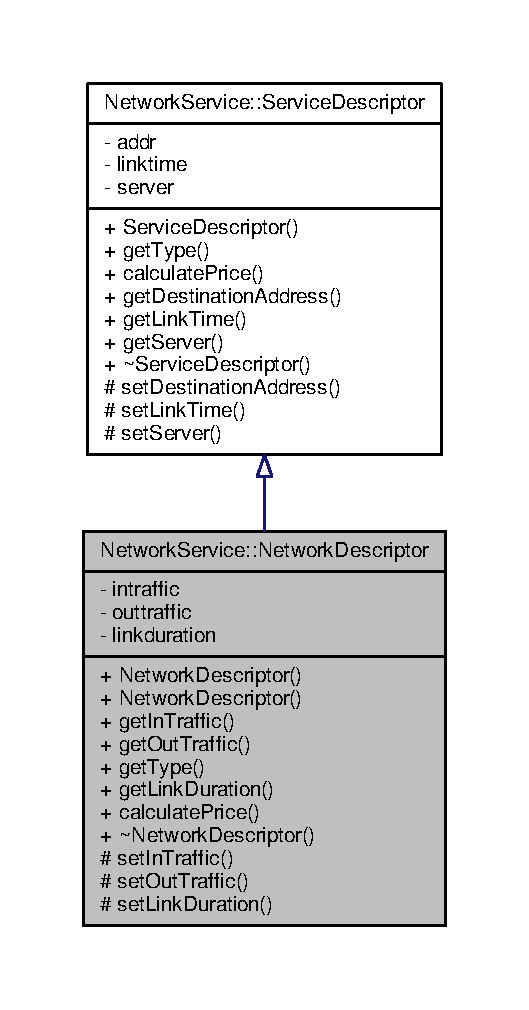
\includegraphics[width=254pt]{class_network_service_1_1_network_descriptor__inherit__graph}
\end{center}
\end{figure}


Граф связей класса Network\+Service\+:\+:Network\+Descriptor\+:\nopagebreak
\begin{figure}[H]
\begin{center}
\leavevmode
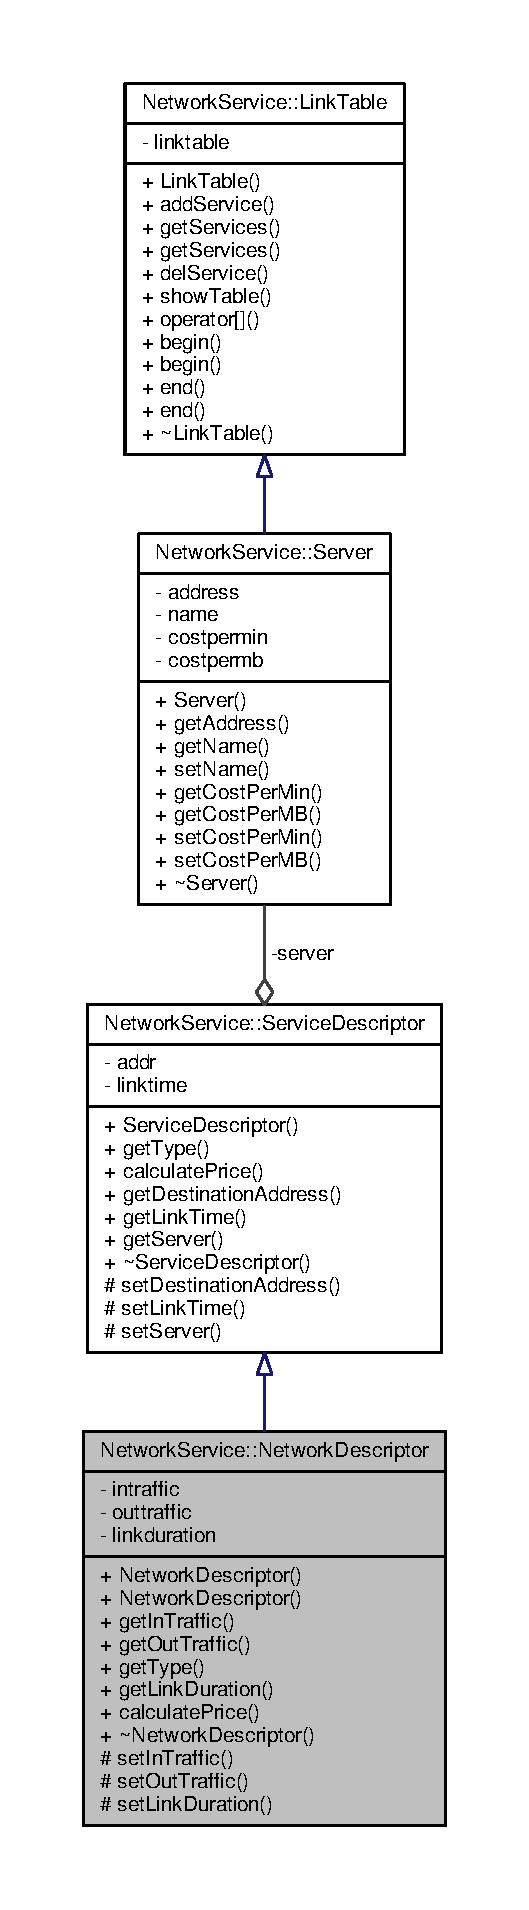
\includegraphics[height=550pt]{class_network_service_1_1_network_descriptor__coll__graph}
\end{center}
\end{figure}
\subsection*{Открытые члены}
\begin{DoxyCompactItemize}
\item 
\hyperlink{class_network_service_1_1_network_descriptor_a320bf7222afe75a0d132f1e51f22afd9}{Network\+Descriptor} ()
\item 
\hyperlink{class_network_service_1_1_network_descriptor_a06cc19962f4a5da19bb8bd7f3bdd9b8a}{Network\+Descriptor} (ulong \hyperlink{class_network_service_1_1_network_descriptor_ac4fc85cab905739a9513fcfd06ca0453}{intraffic}, ulong \hyperlink{class_network_service_1_1_network_descriptor_a109969d9199b67144184e1b296406edc}{outtraffic}, ulong address, \hyperlink{networkservice_8h_ac877dfabb0f4f6a8184aa821b447e81d}{ftimepoint} \&\hyperlink{class_network_service_1_1_service_descriptor_a08bfd17afce0cba1954d30bd76a14df4}{linktime}, \hyperlink{networkservice_8h_a476cc728ef971cba9111c75ea41a760a}{fduration} \&\hyperlink{class_network_service_1_1_network_descriptor_a30c7b2914f9a815341c0d11653f378db}{linkduration}, \hyperlink{class_network_service_1_1_server}{Server} $\ast$\hyperlink{class_network_service_1_1_service_descriptor_ad504b32ced44a75e0e02ea961d9434c4}{server})
\begin{DoxyCompactList}\small\item\em Создает запись об оказанной услуге, основываясь на параметрах \end{DoxyCompactList}\item 
ulong \hyperlink{class_network_service_1_1_network_descriptor_ad8d2c236158fd870ce202b03d07ce202}{get\+In\+Traffic} () const 
\begin{DoxyCompactList}\small\item\em Получение количества полученных данных \end{DoxyCompactList}\item 
ulong \hyperlink{class_network_service_1_1_network_descriptor_adbc216cb7c97d45161f5ec7c7c5a1aa7}{get\+Out\+Traffic} () const 
\begin{DoxyCompactList}\small\item\em Получение количества отправленных данных \end{DoxyCompactList}\item 
std\+::string \hyperlink{class_network_service_1_1_network_descriptor_abef35df6ca05d7b0ed9e3c0385b9a02a}{get\+Type} () const 
\begin{DoxyCompactList}\small\item\em Получение названия типа услуги \end{DoxyCompactList}\item 
const \hyperlink{networkservice_8h_a476cc728ef971cba9111c75ea41a760a}{fduration} \& \hyperlink{class_network_service_1_1_network_descriptor_a21523ecd4dfc2b54873cefd02bc1fb80}{get\+Link\+Duration} () const 
\begin{DoxyCompactList}\small\item\em Получение продолжительности связи \end{DoxyCompactList}\item 
ulong \hyperlink{class_network_service_1_1_network_descriptor_a515f9b5e56c7027101fcb000e9be96a2}{calculate\+Price} () const 
\begin{DoxyCompactList}\small\item\em Рассчет стоимости оказанных услуг \end{DoxyCompactList}\item 
virtual \hyperlink{class_network_service_1_1_network_descriptor_a2bdb0f0cc2aaec9cf58359f1598ea1ee}{$\sim$\+Network\+Descriptor} ()
\end{DoxyCompactItemize}
\subsection*{Защищенные члены}
\begin{DoxyCompactItemize}
\item 
void \hyperlink{class_network_service_1_1_network_descriptor_a93fd081bae34302f1ab259c2c33a8ea8}{set\+In\+Traffic} (ulong \hyperlink{class_network_service_1_1_network_descriptor_ac4fc85cab905739a9513fcfd06ca0453}{intraffic})
\begin{DoxyCompactList}\small\item\em Установка количества полученных данных \end{DoxyCompactList}\item 
void \hyperlink{class_network_service_1_1_network_descriptor_afaa15f0c88bb871378cbd65fc39449ab}{set\+Out\+Traffic} (ulong \hyperlink{class_network_service_1_1_network_descriptor_a109969d9199b67144184e1b296406edc}{outtraffic})
\begin{DoxyCompactList}\small\item\em Установка количества отправленных данных \end{DoxyCompactList}\item 
void \hyperlink{class_network_service_1_1_network_descriptor_aa72594b531998aba59d5586acdfab788}{set\+Link\+Duration} (\hyperlink{networkservice_8h_a476cc728ef971cba9111c75ea41a760a}{fduration} \&ld)
\begin{DoxyCompactList}\small\item\em Установка продолжительности связи \end{DoxyCompactList}\end{DoxyCompactItemize}
\subsection*{Закрытые данные}
\begin{DoxyCompactItemize}
\item 
ulong \hyperlink{class_network_service_1_1_network_descriptor_ac4fc85cab905739a9513fcfd06ca0453}{intraffic}
\item 
ulong \hyperlink{class_network_service_1_1_network_descriptor_a109969d9199b67144184e1b296406edc}{outtraffic}
\begin{DoxyCompactList}\small\item\em Количество переданной и отправленной информации \end{DoxyCompactList}\item 
\hyperlink{networkservice_8h_a476cc728ef971cba9111c75ea41a760a}{fduration} \hyperlink{class_network_service_1_1_network_descriptor_a30c7b2914f9a815341c0d11653f378db}{linkduration}
\begin{DoxyCompactList}\small\item\em Продолжительность связи \end{DoxyCompactList}\end{DoxyCompactItemize}


\subsection{Подробное описание}
Описатель сервиса \char`\"{}сеть\char`\"{}, наследуется от \hyperlink{class_network_service_1_1_service_descriptor}{Service\+Descriptor}. 

\subsection{Конструктор(ы)}
\hypertarget{class_network_service_1_1_network_descriptor_a320bf7222afe75a0d132f1e51f22afd9}{}\index{Network\+Service\+::\+Network\+Descriptor@{Network\+Service\+::\+Network\+Descriptor}!Network\+Descriptor@{Network\+Descriptor}}
\index{Network\+Descriptor@{Network\+Descriptor}!Network\+Service\+::\+Network\+Descriptor@{Network\+Service\+::\+Network\+Descriptor}}
\subsubsection[{Network\+Descriptor}]{\setlength{\rightskip}{0pt plus 5cm}Network\+Descriptor\+::\+Network\+Descriptor (
\begin{DoxyParamCaption}
{}
\end{DoxyParamCaption}
)}\label{class_network_service_1_1_network_descriptor_a320bf7222afe75a0d132f1e51f22afd9}
\hypertarget{class_network_service_1_1_network_descriptor_a06cc19962f4a5da19bb8bd7f3bdd9b8a}{}\index{Network\+Service\+::\+Network\+Descriptor@{Network\+Service\+::\+Network\+Descriptor}!Network\+Descriptor@{Network\+Descriptor}}
\index{Network\+Descriptor@{Network\+Descriptor}!Network\+Service\+::\+Network\+Descriptor@{Network\+Service\+::\+Network\+Descriptor}}
\subsubsection[{Network\+Descriptor}]{\setlength{\rightskip}{0pt plus 5cm}Network\+Descriptor\+::\+Network\+Descriptor (
\begin{DoxyParamCaption}
\item[{ulong}]{intraffic, }
\item[{ulong}]{outtraffic, }
\item[{ulong}]{address, }
\item[{{\bf ftimepoint} \&}]{linktime, }
\item[{{\bf fduration} \&}]{linkduration, }
\item[{{\bf Server} $\ast$}]{server}
\end{DoxyParamCaption}
)}\label{class_network_service_1_1_network_descriptor_a06cc19962f4a5da19bb8bd7f3bdd9b8a}


Создает запись об оказанной услуге, основываясь на параметрах 


\begin{DoxyParams}{Аргументы}
{\em intraffic} & Количество полученной информации (в M\+B) \\
\hline
{\em outtraffic} & Количество переданной информации (в M\+B) \\
\hline
{\em address} & I\+P адрес назначения \\
\hline
{\em linktime} & Время оказания услуги \\
\hline
{\em linkduration} & Продолжительность связи \\
\hline
{\em server} & Указатель на сервер (объект \hyperlink{class_network_service_1_1_server}{Server}), оказывающий услугу \\
\hline
\end{DoxyParams}
\hypertarget{class_network_service_1_1_network_descriptor_a2bdb0f0cc2aaec9cf58359f1598ea1ee}{}\index{Network\+Service\+::\+Network\+Descriptor@{Network\+Service\+::\+Network\+Descriptor}!````~Network\+Descriptor@{$\sim$\+Network\+Descriptor}}
\index{````~Network\+Descriptor@{$\sim$\+Network\+Descriptor}!Network\+Service\+::\+Network\+Descriptor@{Network\+Service\+::\+Network\+Descriptor}}
\subsubsection[{$\sim$\+Network\+Descriptor}]{\setlength{\rightskip}{0pt plus 5cm}Network\+Descriptor\+::$\sim$\+Network\+Descriptor (
\begin{DoxyParamCaption}
{}
\end{DoxyParamCaption}
)\hspace{0.3cm}{\ttfamily [virtual]}}\label{class_network_service_1_1_network_descriptor_a2bdb0f0cc2aaec9cf58359f1598ea1ee}


\subsection{Методы}
\hypertarget{class_network_service_1_1_network_descriptor_a515f9b5e56c7027101fcb000e9be96a2}{}\index{Network\+Service\+::\+Network\+Descriptor@{Network\+Service\+::\+Network\+Descriptor}!calculate\+Price@{calculate\+Price}}
\index{calculate\+Price@{calculate\+Price}!Network\+Service\+::\+Network\+Descriptor@{Network\+Service\+::\+Network\+Descriptor}}
\subsubsection[{calculate\+Price}]{\setlength{\rightskip}{0pt plus 5cm}ulong Network\+Descriptor\+::calculate\+Price (
\begin{DoxyParamCaption}
{}
\end{DoxyParamCaption}
) const\hspace{0.3cm}{\ttfamily [virtual]}}\label{class_network_service_1_1_network_descriptor_a515f9b5e56c7027101fcb000e9be96a2}


Рассчет стоимости оказанных услуг 

\begin{DoxyReturn}{Возвращает}
Стоимость оказанных услуг
\end{DoxyReturn}
Рассчет стоимости оказанных услуг, на основании стоимости 1 минуты и 1\+M\+B, установленной сервером 

Замещает \hyperlink{class_network_service_1_1_service_descriptor_aa2da86b27ac53d8acb1eddf3723a1e44}{Network\+Service\+::\+Service\+Descriptor}.

\hypertarget{class_network_service_1_1_network_descriptor_ad8d2c236158fd870ce202b03d07ce202}{}\index{Network\+Service\+::\+Network\+Descriptor@{Network\+Service\+::\+Network\+Descriptor}!get\+In\+Traffic@{get\+In\+Traffic}}
\index{get\+In\+Traffic@{get\+In\+Traffic}!Network\+Service\+::\+Network\+Descriptor@{Network\+Service\+::\+Network\+Descriptor}}
\subsubsection[{get\+In\+Traffic}]{\setlength{\rightskip}{0pt plus 5cm}ulong Network\+Descriptor\+::get\+In\+Traffic (
\begin{DoxyParamCaption}
{}
\end{DoxyParamCaption}
) const}\label{class_network_service_1_1_network_descriptor_ad8d2c236158fd870ce202b03d07ce202}


Получение количества полученных данных 

\begin{DoxyReturn}{Возвращает}
Количество полученных данных (в M\+B) 
\end{DoxyReturn}
\hypertarget{class_network_service_1_1_network_descriptor_a21523ecd4dfc2b54873cefd02bc1fb80}{}\index{Network\+Service\+::\+Network\+Descriptor@{Network\+Service\+::\+Network\+Descriptor}!get\+Link\+Duration@{get\+Link\+Duration}}
\index{get\+Link\+Duration@{get\+Link\+Duration}!Network\+Service\+::\+Network\+Descriptor@{Network\+Service\+::\+Network\+Descriptor}}
\subsubsection[{get\+Link\+Duration}]{\setlength{\rightskip}{0pt plus 5cm}const {\bf fduration} \& Network\+Descriptor\+::get\+Link\+Duration (
\begin{DoxyParamCaption}
{}
\end{DoxyParamCaption}
) const}\label{class_network_service_1_1_network_descriptor_a21523ecd4dfc2b54873cefd02bc1fb80}


Получение продолжительности связи 

\begin{DoxyReturn}{Возвращает}
Ссылка на объект fduration 
\end{DoxyReturn}
\hypertarget{class_network_service_1_1_network_descriptor_adbc216cb7c97d45161f5ec7c7c5a1aa7}{}\index{Network\+Service\+::\+Network\+Descriptor@{Network\+Service\+::\+Network\+Descriptor}!get\+Out\+Traffic@{get\+Out\+Traffic}}
\index{get\+Out\+Traffic@{get\+Out\+Traffic}!Network\+Service\+::\+Network\+Descriptor@{Network\+Service\+::\+Network\+Descriptor}}
\subsubsection[{get\+Out\+Traffic}]{\setlength{\rightskip}{0pt plus 5cm}ulong Network\+Descriptor\+::get\+Out\+Traffic (
\begin{DoxyParamCaption}
{}
\end{DoxyParamCaption}
) const}\label{class_network_service_1_1_network_descriptor_adbc216cb7c97d45161f5ec7c7c5a1aa7}


Получение количества отправленных данных 

\begin{DoxyReturn}{Возвращает}
Количество отправленных данных M\+B 
\end{DoxyReturn}
\hypertarget{class_network_service_1_1_network_descriptor_abef35df6ca05d7b0ed9e3c0385b9a02a}{}\index{Network\+Service\+::\+Network\+Descriptor@{Network\+Service\+::\+Network\+Descriptor}!get\+Type@{get\+Type}}
\index{get\+Type@{get\+Type}!Network\+Service\+::\+Network\+Descriptor@{Network\+Service\+::\+Network\+Descriptor}}
\subsubsection[{get\+Type}]{\setlength{\rightskip}{0pt plus 5cm}std\+::string Network\+Descriptor\+::get\+Type (
\begin{DoxyParamCaption}
{}
\end{DoxyParamCaption}
) const\hspace{0.3cm}{\ttfamily [virtual]}}\label{class_network_service_1_1_network_descriptor_abef35df6ca05d7b0ed9e3c0385b9a02a}


Получение названия типа услуги 

\begin{DoxyReturn}{Возвращает}
Название типа услуги (строка \char`\"{}\+Network\char`\"{}) 
\end{DoxyReturn}


Замещает \hyperlink{class_network_service_1_1_service_descriptor_ac09d5d704a67a7ab2df6d925751ee5cc}{Network\+Service\+::\+Service\+Descriptor}.

\hypertarget{class_network_service_1_1_network_descriptor_a93fd081bae34302f1ab259c2c33a8ea8}{}\index{Network\+Service\+::\+Network\+Descriptor@{Network\+Service\+::\+Network\+Descriptor}!set\+In\+Traffic@{set\+In\+Traffic}}
\index{set\+In\+Traffic@{set\+In\+Traffic}!Network\+Service\+::\+Network\+Descriptor@{Network\+Service\+::\+Network\+Descriptor}}
\subsubsection[{set\+In\+Traffic}]{\setlength{\rightskip}{0pt plus 5cm}void Network\+Descriptor\+::set\+In\+Traffic (
\begin{DoxyParamCaption}
\item[{ulong}]{intraffic}
\end{DoxyParamCaption}
)\hspace{0.3cm}{\ttfamily [protected]}}\label{class_network_service_1_1_network_descriptor_a93fd081bae34302f1ab259c2c33a8ea8}


Установка количества полученных данных 


\begin{DoxyParams}{Аргументы}
{\em intraffic} & Количество полученных данных \\
\hline
\end{DoxyParams}
\hypertarget{class_network_service_1_1_network_descriptor_aa72594b531998aba59d5586acdfab788}{}\index{Network\+Service\+::\+Network\+Descriptor@{Network\+Service\+::\+Network\+Descriptor}!set\+Link\+Duration@{set\+Link\+Duration}}
\index{set\+Link\+Duration@{set\+Link\+Duration}!Network\+Service\+::\+Network\+Descriptor@{Network\+Service\+::\+Network\+Descriptor}}
\subsubsection[{set\+Link\+Duration}]{\setlength{\rightskip}{0pt plus 5cm}void Network\+Descriptor\+::set\+Link\+Duration (
\begin{DoxyParamCaption}
\item[{{\bf fduration} \&}]{ld}
\end{DoxyParamCaption}
)\hspace{0.3cm}{\ttfamily [protected]}}\label{class_network_service_1_1_network_descriptor_aa72594b531998aba59d5586acdfab788}


Установка продолжительности связи 


\begin{DoxyParams}{Аргументы}
{\em ld} & Ссылка на объект fduration, содержащий информацию о продолжительности связи \\
\hline
\end{DoxyParams}
\hypertarget{class_network_service_1_1_network_descriptor_afaa15f0c88bb871378cbd65fc39449ab}{}\index{Network\+Service\+::\+Network\+Descriptor@{Network\+Service\+::\+Network\+Descriptor}!set\+Out\+Traffic@{set\+Out\+Traffic}}
\index{set\+Out\+Traffic@{set\+Out\+Traffic}!Network\+Service\+::\+Network\+Descriptor@{Network\+Service\+::\+Network\+Descriptor}}
\subsubsection[{set\+Out\+Traffic}]{\setlength{\rightskip}{0pt plus 5cm}void Network\+Descriptor\+::set\+Out\+Traffic (
\begin{DoxyParamCaption}
\item[{ulong}]{outtraffic}
\end{DoxyParamCaption}
)\hspace{0.3cm}{\ttfamily [protected]}}\label{class_network_service_1_1_network_descriptor_afaa15f0c88bb871378cbd65fc39449ab}


Установка количества отправленных данных 


\begin{DoxyParams}{Аргументы}
{\em outtraffic} & Количество отправленных данных \\
\hline
\end{DoxyParams}


\subsection{Данные класса}
\hypertarget{class_network_service_1_1_network_descriptor_ac4fc85cab905739a9513fcfd06ca0453}{}\index{Network\+Service\+::\+Network\+Descriptor@{Network\+Service\+::\+Network\+Descriptor}!intraffic@{intraffic}}
\index{intraffic@{intraffic}!Network\+Service\+::\+Network\+Descriptor@{Network\+Service\+::\+Network\+Descriptor}}
\subsubsection[{intraffic}]{\setlength{\rightskip}{0pt plus 5cm}ulong Network\+Service\+::\+Network\+Descriptor\+::intraffic\hspace{0.3cm}{\ttfamily [private]}}\label{class_network_service_1_1_network_descriptor_ac4fc85cab905739a9513fcfd06ca0453}
\hypertarget{class_network_service_1_1_network_descriptor_a30c7b2914f9a815341c0d11653f378db}{}\index{Network\+Service\+::\+Network\+Descriptor@{Network\+Service\+::\+Network\+Descriptor}!linkduration@{linkduration}}
\index{linkduration@{linkduration}!Network\+Service\+::\+Network\+Descriptor@{Network\+Service\+::\+Network\+Descriptor}}
\subsubsection[{linkduration}]{\setlength{\rightskip}{0pt plus 5cm}{\bf fduration} Network\+Service\+::\+Network\+Descriptor\+::linkduration\hspace{0.3cm}{\ttfamily [private]}}\label{class_network_service_1_1_network_descriptor_a30c7b2914f9a815341c0d11653f378db}


Продолжительность связи 

\hypertarget{class_network_service_1_1_network_descriptor_a109969d9199b67144184e1b296406edc}{}\index{Network\+Service\+::\+Network\+Descriptor@{Network\+Service\+::\+Network\+Descriptor}!outtraffic@{outtraffic}}
\index{outtraffic@{outtraffic}!Network\+Service\+::\+Network\+Descriptor@{Network\+Service\+::\+Network\+Descriptor}}
\subsubsection[{outtraffic}]{\setlength{\rightskip}{0pt plus 5cm}ulong Network\+Service\+::\+Network\+Descriptor\+::outtraffic\hspace{0.3cm}{\ttfamily [private]}}\label{class_network_service_1_1_network_descriptor_a109969d9199b67144184e1b296406edc}


Количество переданной и отправленной информации 



Объявления и описания членов классов находятся в файлах\+:\begin{DoxyCompactItemize}
\item 
Network\+Service\+Lib/\hyperlink{networkdescriptor_8h}{networkdescriptor.\+h}\item 
Network\+Service\+Lib/\hyperlink{networkdescriptor_8cpp}{networkdescriptor.\+cpp}\end{DoxyCompactItemize}

\hypertarget{class_network_service_1_1_post_descriptor}{}\section{Класс Network\+Service\+:\+:Post\+Descriptor}
\label{class_network_service_1_1_post_descriptor}\index{Network\+Service\+::\+Post\+Descriptor@{Network\+Service\+::\+Post\+Descriptor}}


Описатель сервиса \char`\"{}почта\char`\"{}, наследуемый от \hyperlink{class_network_service_1_1_service_descriptor}{Service\+Descriptor}.  




{\ttfamily \#include $<$postdescriptor.\+h$>$}



Граф наследования\+:Network\+Service\+:\+:Post\+Descriptor\+:\nopagebreak
\begin{figure}[H]
\begin{center}
\leavevmode
\includegraphics[height=550pt]{class_network_service_1_1_post_descriptor__inherit__graph}
\end{center}
\end{figure}


Граф связей класса Network\+Service\+:\+:Post\+Descriptor\+:\nopagebreak
\begin{figure}[H]
\begin{center}
\leavevmode
\includegraphics[height=550pt]{class_network_service_1_1_post_descriptor__coll__graph}
\end{center}
\end{figure}
\subsection*{Открытые члены}
\begin{DoxyCompactItemize}
\item 
\hyperlink{class_network_service_1_1_post_descriptor_a7c6bd39a757d05812d5ee8f3faea133a}{Post\+Descriptor} ()
\item 
\hyperlink{class_network_service_1_1_post_descriptor_ac888b36a88d706220479595328e8f2cb}{Post\+Descriptor} (ulong \hyperlink{class_network_service_1_1_post_descriptor_ae2eef559828a42ec299ab59711f88e59}{traffic}, \hyperlink{namespace_network_service_abe1196dad9e8afcbc5c6b38196ce2c65}{Direction} \hyperlink{class_network_service_1_1_post_descriptor_a04faf66e747b2d4f2d89bf1e92f4ab5c}{direction}, ulong address, \hyperlink{networkservice_8h_ac877dfabb0f4f6a8184aa821b447e81d}{ftimepoint} \&\hyperlink{class_network_service_1_1_service_descriptor_a08bfd17afce0cba1954d30bd76a14df4}{linktime}, \hyperlink{class_network_service_1_1_server}{Server} $\ast$\hyperlink{class_network_service_1_1_service_descriptor_ad504b32ced44a75e0e02ea961d9434c4}{server})
\begin{DoxyCompactList}\small\item\em Создает запись об оказанной услуге, основываясь на параметрах \end{DoxyCompactList}\item 
\hyperlink{namespace_network_service_abe1196dad9e8afcbc5c6b38196ce2c65}{Direction} \hyperlink{class_network_service_1_1_post_descriptor_a09d005d77c03866e7875f4df0dcffad2}{get\+Direction} () const 
\begin{DoxyCompactList}\small\item\em Получить направление передачи данных \end{DoxyCompactList}\item 
ulong \hyperlink{class_network_service_1_1_post_descriptor_a3b859050d7ca47084a751b2be4da192c}{get\+Traffic} () const 
\begin{DoxyCompactList}\small\item\em Получить количество переданных данных \end{DoxyCompactList}\item 
virtual std\+::string \hyperlink{class_network_service_1_1_post_descriptor_a91b6330d604d4866c85c32187f131431}{get\+Type} () const 
\begin{DoxyCompactList}\small\item\em Получение названия типа услуги \end{DoxyCompactList}\item 
virtual ulong \hyperlink{class_network_service_1_1_post_descriptor_ae88dfdc2d12299b6d3b14786d16e3251}{calculate\+Price} () const 
\begin{DoxyCompactList}\small\item\em Рассчет стоимости оказанных услуг \end{DoxyCompactList}\item 
virtual \hyperlink{class_network_service_1_1_post_descriptor_a4b6701e1d070e3d0425840d6597bc505}{$\sim$\+Post\+Descriptor} ()
\end{DoxyCompactItemize}
\subsection*{Защищенные члены}
\begin{DoxyCompactItemize}
\item 
void \hyperlink{class_network_service_1_1_post_descriptor_a5e3e03cbe0e31397bed9e17428348bd1}{set\+Traffic} (ulong)
\begin{DoxyCompactList}\small\item\em Изменения количество переданной информации \end{DoxyCompactList}\item 
void \hyperlink{class_network_service_1_1_post_descriptor_ab976b83349507b5e6841fcbc2ddc9edd}{set\+Direction} (\hyperlink{namespace_network_service_abe1196dad9e8afcbc5c6b38196ce2c65}{Direction})
\begin{DoxyCompactList}\small\item\em Изменения направления передачи данных \end{DoxyCompactList}\end{DoxyCompactItemize}
\subsection*{Закрытые данные}
\begin{DoxyCompactItemize}
\item 
ulong \hyperlink{class_network_service_1_1_post_descriptor_ae2eef559828a42ec299ab59711f88e59}{traffic}
\begin{DoxyCompactList}\small\item\em Количество отправленных/полученных данных в M\+B. \end{DoxyCompactList}\item 
\hyperlink{namespace_network_service_abe1196dad9e8afcbc5c6b38196ce2c65}{Direction} \hyperlink{class_network_service_1_1_post_descriptor_a04faf66e747b2d4f2d89bf1e92f4ab5c}{direction}
\begin{DoxyCompactList}\small\item\em Направление передачи данных \end{DoxyCompactList}\end{DoxyCompactItemize}


\subsection{Подробное описание}
Описатель сервиса \char`\"{}почта\char`\"{}, наследуемый от \hyperlink{class_network_service_1_1_service_descriptor}{Service\+Descriptor}. 

\subsection{Конструктор(ы)}
\hypertarget{class_network_service_1_1_post_descriptor_a7c6bd39a757d05812d5ee8f3faea133a}{}\index{Network\+Service\+::\+Post\+Descriptor@{Network\+Service\+::\+Post\+Descriptor}!Post\+Descriptor@{Post\+Descriptor}}
\index{Post\+Descriptor@{Post\+Descriptor}!Network\+Service\+::\+Post\+Descriptor@{Network\+Service\+::\+Post\+Descriptor}}
\subsubsection[{Post\+Descriptor}]{\setlength{\rightskip}{0pt plus 5cm}Post\+Descriptor\+::\+Post\+Descriptor (
\begin{DoxyParamCaption}
{}
\end{DoxyParamCaption}
)}\label{class_network_service_1_1_post_descriptor_a7c6bd39a757d05812d5ee8f3faea133a}
\hypertarget{class_network_service_1_1_post_descriptor_ac888b36a88d706220479595328e8f2cb}{}\index{Network\+Service\+::\+Post\+Descriptor@{Network\+Service\+::\+Post\+Descriptor}!Post\+Descriptor@{Post\+Descriptor}}
\index{Post\+Descriptor@{Post\+Descriptor}!Network\+Service\+::\+Post\+Descriptor@{Network\+Service\+::\+Post\+Descriptor}}
\subsubsection[{Post\+Descriptor}]{\setlength{\rightskip}{0pt plus 5cm}Post\+Descriptor\+::\+Post\+Descriptor (
\begin{DoxyParamCaption}
\item[{ulong}]{traffic, }
\item[{{\bf Direction}}]{direction, }
\item[{ulong}]{address, }
\item[{{\bf ftimepoint} \&}]{linktime, }
\item[{{\bf Server} $\ast$}]{server}
\end{DoxyParamCaption}
)}\label{class_network_service_1_1_post_descriptor_ac888b36a88d706220479595328e8f2cb}


Создает запись об оказанной услуге, основываясь на параметрах 


\begin{DoxyParams}{Аргументы}
{\em traffic} & Количество переданных данных в M\+B \\
\hline
{\em direction} & Направление передачи \\
\hline
{\em address} & Адрес назначения \\
\hline
{\em linktime} & Времи оказания услуги \\
\hline
{\em server} & Указатель на сервер (объект \hyperlink{class_network_service_1_1_server}{Server}), оказывающий услугу \\
\hline
\end{DoxyParams}
\hypertarget{class_network_service_1_1_post_descriptor_a4b6701e1d070e3d0425840d6597bc505}{}\index{Network\+Service\+::\+Post\+Descriptor@{Network\+Service\+::\+Post\+Descriptor}!````~Post\+Descriptor@{$\sim$\+Post\+Descriptor}}
\index{````~Post\+Descriptor@{$\sim$\+Post\+Descriptor}!Network\+Service\+::\+Post\+Descriptor@{Network\+Service\+::\+Post\+Descriptor}}
\subsubsection[{$\sim$\+Post\+Descriptor}]{\setlength{\rightskip}{0pt plus 5cm}Post\+Descriptor\+::$\sim$\+Post\+Descriptor (
\begin{DoxyParamCaption}
{}
\end{DoxyParamCaption}
)\hspace{0.3cm}{\ttfamily [virtual]}}\label{class_network_service_1_1_post_descriptor_a4b6701e1d070e3d0425840d6597bc505}


\subsection{Методы}
\hypertarget{class_network_service_1_1_post_descriptor_ae88dfdc2d12299b6d3b14786d16e3251}{}\index{Network\+Service\+::\+Post\+Descriptor@{Network\+Service\+::\+Post\+Descriptor}!calculate\+Price@{calculate\+Price}}
\index{calculate\+Price@{calculate\+Price}!Network\+Service\+::\+Post\+Descriptor@{Network\+Service\+::\+Post\+Descriptor}}
\subsubsection[{calculate\+Price}]{\setlength{\rightskip}{0pt plus 5cm}ulong Post\+Descriptor\+::calculate\+Price (
\begin{DoxyParamCaption}
{}
\end{DoxyParamCaption}
) const\hspace{0.3cm}{\ttfamily [virtual]}}\label{class_network_service_1_1_post_descriptor_ae88dfdc2d12299b6d3b14786d16e3251}


Рассчет стоимости оказанных услуг 

\begin{DoxyReturn}{Возвращает}
Стоимость оказанных услуг
\end{DoxyReturn}
Рассчет стоимости оказанных услуг, на основании стоимости 1\+M\+B, установленной сервером 

Замещает \hyperlink{class_network_service_1_1_service_descriptor_aa2da86b27ac53d8acb1eddf3723a1e44}{Network\+Service\+::\+Service\+Descriptor}.



Переопределяется в \hyperlink{class_network_service_1_1_file_descriptor_a2c480da1613f7072d3113082d1f8cc54}{Network\+Service\+::\+File\+Descriptor}.

\hypertarget{class_network_service_1_1_post_descriptor_a09d005d77c03866e7875f4df0dcffad2}{}\index{Network\+Service\+::\+Post\+Descriptor@{Network\+Service\+::\+Post\+Descriptor}!get\+Direction@{get\+Direction}}
\index{get\+Direction@{get\+Direction}!Network\+Service\+::\+Post\+Descriptor@{Network\+Service\+::\+Post\+Descriptor}}
\subsubsection[{get\+Direction}]{\setlength{\rightskip}{0pt plus 5cm}{\bf Direction} Post\+Descriptor\+::get\+Direction (
\begin{DoxyParamCaption}
{}
\end{DoxyParamCaption}
) const}\label{class_network_service_1_1_post_descriptor_a09d005d77c03866e7875f4df0dcffad2}


Получить направление передачи данных 

\begin{DoxyReturn}{Возвращает}
Направление передачи данных 
\end{DoxyReturn}
\hypertarget{class_network_service_1_1_post_descriptor_a3b859050d7ca47084a751b2be4da192c}{}\index{Network\+Service\+::\+Post\+Descriptor@{Network\+Service\+::\+Post\+Descriptor}!get\+Traffic@{get\+Traffic}}
\index{get\+Traffic@{get\+Traffic}!Network\+Service\+::\+Post\+Descriptor@{Network\+Service\+::\+Post\+Descriptor}}
\subsubsection[{get\+Traffic}]{\setlength{\rightskip}{0pt plus 5cm}ulong Post\+Descriptor\+::get\+Traffic (
\begin{DoxyParamCaption}
{}
\end{DoxyParamCaption}
) const}\label{class_network_service_1_1_post_descriptor_a3b859050d7ca47084a751b2be4da192c}


Получить количество переданных данных 

\begin{DoxyReturn}{Возвращает}
Количество переданных данных в M\+B 
\end{DoxyReturn}
\hypertarget{class_network_service_1_1_post_descriptor_a91b6330d604d4866c85c32187f131431}{}\index{Network\+Service\+::\+Post\+Descriptor@{Network\+Service\+::\+Post\+Descriptor}!get\+Type@{get\+Type}}
\index{get\+Type@{get\+Type}!Network\+Service\+::\+Post\+Descriptor@{Network\+Service\+::\+Post\+Descriptor}}
\subsubsection[{get\+Type}]{\setlength{\rightskip}{0pt plus 5cm}std\+::string Post\+Descriptor\+::get\+Type (
\begin{DoxyParamCaption}
{}
\end{DoxyParamCaption}
) const\hspace{0.3cm}{\ttfamily [virtual]}}\label{class_network_service_1_1_post_descriptor_a91b6330d604d4866c85c32187f131431}


Получение названия типа услуги 

\begin{DoxyReturn}{Возвращает}
Название типа услуги (строка \char`\"{}\+Post\char`\"{}) 
\end{DoxyReturn}


Замещает \hyperlink{class_network_service_1_1_service_descriptor_ac09d5d704a67a7ab2df6d925751ee5cc}{Network\+Service\+::\+Service\+Descriptor}.



Переопределяется в \hyperlink{class_network_service_1_1_file_descriptor_a68270f753630bf3ac34c621a56e4f6f7}{Network\+Service\+::\+File\+Descriptor}.

\hypertarget{class_network_service_1_1_post_descriptor_ab976b83349507b5e6841fcbc2ddc9edd}{}\index{Network\+Service\+::\+Post\+Descriptor@{Network\+Service\+::\+Post\+Descriptor}!set\+Direction@{set\+Direction}}
\index{set\+Direction@{set\+Direction}!Network\+Service\+::\+Post\+Descriptor@{Network\+Service\+::\+Post\+Descriptor}}
\subsubsection[{set\+Direction}]{\setlength{\rightskip}{0pt plus 5cm}void Post\+Descriptor\+::set\+Direction (
\begin{DoxyParamCaption}
\item[{{\bf Direction}}]{d}
\end{DoxyParamCaption}
)\hspace{0.3cm}{\ttfamily [protected]}}\label{class_network_service_1_1_post_descriptor_ab976b83349507b5e6841fcbc2ddc9edd}


Изменения направления передачи данных 


\begin{DoxyParams}{Аргументы}
{\em d} & Направление передачи \\
\hline
\end{DoxyParams}
\hypertarget{class_network_service_1_1_post_descriptor_a5e3e03cbe0e31397bed9e17428348bd1}{}\index{Network\+Service\+::\+Post\+Descriptor@{Network\+Service\+::\+Post\+Descriptor}!set\+Traffic@{set\+Traffic}}
\index{set\+Traffic@{set\+Traffic}!Network\+Service\+::\+Post\+Descriptor@{Network\+Service\+::\+Post\+Descriptor}}
\subsubsection[{set\+Traffic}]{\setlength{\rightskip}{0pt plus 5cm}void Post\+Descriptor\+::set\+Traffic (
\begin{DoxyParamCaption}
\item[{ulong}]{t}
\end{DoxyParamCaption}
)\hspace{0.3cm}{\ttfamily [protected]}}\label{class_network_service_1_1_post_descriptor_a5e3e03cbe0e31397bed9e17428348bd1}


Изменения количество переданной информации 


\begin{DoxyParams}{Аргументы}
{\em t} & Количество переданной информации (в M\+B) \\
\hline
\end{DoxyParams}


\subsection{Данные класса}
\hypertarget{class_network_service_1_1_post_descriptor_a04faf66e747b2d4f2d89bf1e92f4ab5c}{}\index{Network\+Service\+::\+Post\+Descriptor@{Network\+Service\+::\+Post\+Descriptor}!direction@{direction}}
\index{direction@{direction}!Network\+Service\+::\+Post\+Descriptor@{Network\+Service\+::\+Post\+Descriptor}}
\subsubsection[{direction}]{\setlength{\rightskip}{0pt plus 5cm}{\bf Direction} Network\+Service\+::\+Post\+Descriptor\+::direction\hspace{0.3cm}{\ttfamily [private]}}\label{class_network_service_1_1_post_descriptor_a04faf66e747b2d4f2d89bf1e92f4ab5c}


Направление передачи данных 

\hypertarget{class_network_service_1_1_post_descriptor_ae2eef559828a42ec299ab59711f88e59}{}\index{Network\+Service\+::\+Post\+Descriptor@{Network\+Service\+::\+Post\+Descriptor}!traffic@{traffic}}
\index{traffic@{traffic}!Network\+Service\+::\+Post\+Descriptor@{Network\+Service\+::\+Post\+Descriptor}}
\subsubsection[{traffic}]{\setlength{\rightskip}{0pt plus 5cm}ulong Network\+Service\+::\+Post\+Descriptor\+::traffic\hspace{0.3cm}{\ttfamily [private]}}\label{class_network_service_1_1_post_descriptor_ae2eef559828a42ec299ab59711f88e59}


Количество отправленных/полученных данных в M\+B. 



Объявления и описания членов классов находятся в файлах\+:\begin{DoxyCompactItemize}
\item 
Network\+Service\+Lib/\hyperlink{postdescriptor_8h}{postdescriptor.\+h}\item 
Network\+Service\+Lib/\hyperlink{postdescriptor_8cpp}{postdescriptor.\+cpp}\end{DoxyCompactItemize}

\hypertarget{class_network_service_1_1_server}{}\section{Класс Network\+Service\+:\+:Server}
\label{class_network_service_1_1_server}\index{Network\+Service\+::\+Server@{Network\+Service\+::\+Server}}


Описатель сервера  




{\ttfamily \#include $<$server.\+h$>$}



Граф наследования\+:Network\+Service\+:\+:Server\+:\nopagebreak
\begin{figure}[H]
\begin{center}
\leavevmode
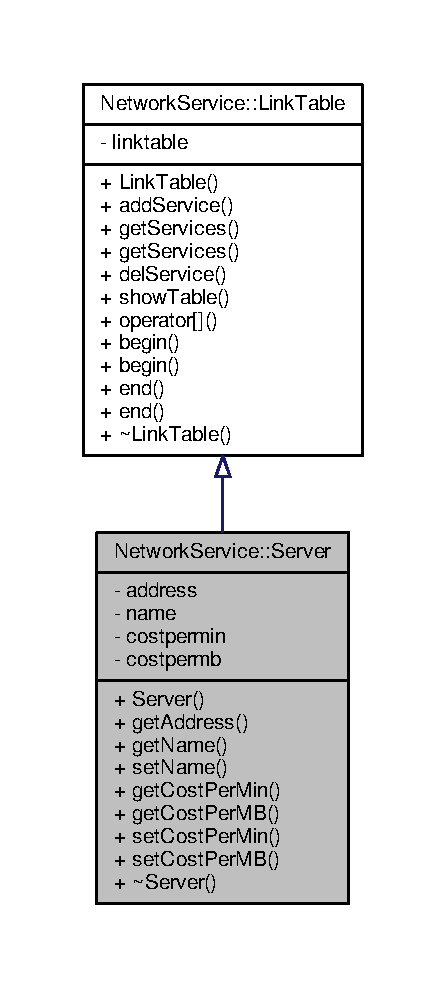
\includegraphics[width=214pt]{class_network_service_1_1_server__inherit__graph}
\end{center}
\end{figure}


Граф связей класса Network\+Service\+:\+:Server\+:\nopagebreak
\begin{figure}[H]
\begin{center}
\leavevmode
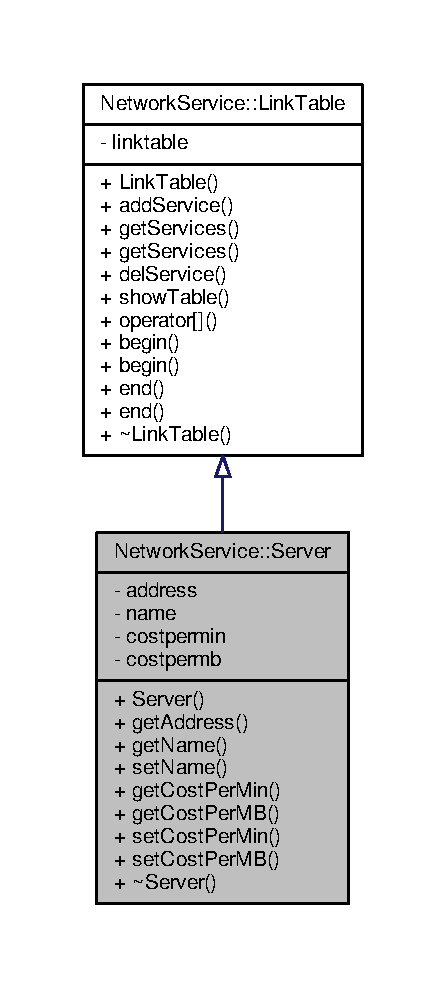
\includegraphics[width=214pt]{class_network_service_1_1_server__coll__graph}
\end{center}
\end{figure}
\subsection*{Открытые члены}
\begin{DoxyCompactItemize}
\item 
\hyperlink{class_network_service_1_1_server_a2d34de4725c705fe2fef379eb5d40f8c}{Server} (ulong \hyperlink{class_network_service_1_1_server_a09382556ff4ab5abc7a79a333ad92329}{address})
\begin{DoxyCompactList}\small\item\em Создание описателя сервиса \end{DoxyCompactList}\item 
ulong \hyperlink{class_network_service_1_1_server_af119e62540303172462f3111784963e9}{get\+Address} () const 
\begin{DoxyCompactList}\small\item\em Получение I\+P сервера \end{DoxyCompactList}\item 
const std\+::string \& \hyperlink{class_network_service_1_1_server_a6dfb5c080e28f814316f641e56383eeb}{get\+Name} () const 
\begin{DoxyCompactList}\small\item\em Получение имени сервера \end{DoxyCompactList}\item 
void \hyperlink{class_network_service_1_1_server_a33076324ad9201dc947be14195a85ad1}{set\+Name} (std\+::string \&\hyperlink{class_network_service_1_1_server_aaab7735b4b5809169ecb92fa66f0bca7}{name})
\begin{DoxyCompactList}\small\item\em Установка имени сервера \end{DoxyCompactList}\item 
ulong \hyperlink{class_network_service_1_1_server_a08126e6a88407ffeacc860588eb6cee4}{get\+Cost\+Per\+Min} () const 
\begin{DoxyCompactList}\small\item\em Получение стоимости 1 минуты связи \end{DoxyCompactList}\item 
ulong \hyperlink{class_network_service_1_1_server_a45d1ea42776ec586c762a2b0b0e5560e}{get\+Cost\+Per\+M\+B} () const 
\begin{DoxyCompactList}\small\item\em Получение стоимости передачи 1\+M\+B данных \end{DoxyCompactList}\item 
void \hyperlink{class_network_service_1_1_server_a41772229229e7994706e6494f6366db8}{set\+Cost\+Per\+Min} (ulong cost)
\begin{DoxyCompactList}\small\item\em Установка стоимости 1 минуты связи \end{DoxyCompactList}\item 
void \hyperlink{class_network_service_1_1_server_a05c94527d60ec19810d7d37bd9c8aaa4}{set\+Cost\+Per\+M\+B} (ulong cost)
\begin{DoxyCompactList}\small\item\em Установка стоимости передачи 1\+M\+B данных \end{DoxyCompactList}\item 
virtual \hyperlink{class_network_service_1_1_server_a097877808f60d35a4f38bf199d5db208}{$\sim$\+Server} ()
\end{DoxyCompactItemize}
\subsection*{Закрытые данные}
\begin{DoxyCompactItemize}
\item 
ulong \hyperlink{class_network_service_1_1_server_a09382556ff4ab5abc7a79a333ad92329}{address}
\begin{DoxyCompactList}\small\item\em I\+P адрес сервера \end{DoxyCompactList}\item 
std\+::string \hyperlink{class_network_service_1_1_server_aaab7735b4b5809169ecb92fa66f0bca7}{name}
\begin{DoxyCompactList}\small\item\em Имя сервера \end{DoxyCompactList}\item 
ulong \hyperlink{class_network_service_1_1_server_a8b24807f5ca15d5348734cf5f4fe96ff}{costpermin}
\item 
ulong \hyperlink{class_network_service_1_1_server_a44f0b3aacbbbbbcf0216974c23d1baf1}{costpermb}
\begin{DoxyCompactList}\small\item\em Стоимость 1 минуты связи и 1\+M\+B переданных данных \end{DoxyCompactList}\end{DoxyCompactItemize}
\subsection*{Друзья}
\begin{DoxyCompactItemize}
\item 
class \hyperlink{class_network_service_1_1_server_a23f25bcc02a0e94c2f5a4188496b04d0}{Application}
\begin{DoxyCompactList}\small\item\em Необходимо для изменения адреса \end{DoxyCompactList}\end{DoxyCompactItemize}
\subsection*{Дополнительные унаследованные члены}


\subsection{Подробное описание}
Описатель сервера 

Описатель сервера. Используется наследование от \hyperlink{class_network_service_1_1_link_table}{Link\+Table} вместо композиции для облегчения работы с итераторами 

\subsection{Конструктор(ы)}
\hypertarget{class_network_service_1_1_server_a2d34de4725c705fe2fef379eb5d40f8c}{}\index{Network\+Service\+::\+Server@{Network\+Service\+::\+Server}!Server@{Server}}
\index{Server@{Server}!Network\+Service\+::\+Server@{Network\+Service\+::\+Server}}
\subsubsection[{Server}]{\setlength{\rightskip}{0pt plus 5cm}Server\+::\+Server (
\begin{DoxyParamCaption}
\item[{ulong}]{address}
\end{DoxyParamCaption}
)\hspace{0.3cm}{\ttfamily [explicit]}}\label{class_network_service_1_1_server_a2d34de4725c705fe2fef379eb5d40f8c}


Создание описателя сервиса 


\begin{DoxyParams}{Аргументы}
{\em address} & I\+P адрес сервера \\
\hline
\end{DoxyParams}
\begin{DoxyWarning}{Предупреждения}
Проверка на правильность и свободность адреса не выполняется 
\end{DoxyWarning}
\hypertarget{class_network_service_1_1_server_a097877808f60d35a4f38bf199d5db208}{}\index{Network\+Service\+::\+Server@{Network\+Service\+::\+Server}!````~Server@{$\sim$\+Server}}
\index{````~Server@{$\sim$\+Server}!Network\+Service\+::\+Server@{Network\+Service\+::\+Server}}
\subsubsection[{$\sim$\+Server}]{\setlength{\rightskip}{0pt plus 5cm}virtual Network\+Service\+::\+Server\+::$\sim$\+Server (
\begin{DoxyParamCaption}
{}
\end{DoxyParamCaption}
)\hspace{0.3cm}{\ttfamily [virtual]}}\label{class_network_service_1_1_server_a097877808f60d35a4f38bf199d5db208}


\subsection{Методы}
\hypertarget{class_network_service_1_1_server_af119e62540303172462f3111784963e9}{}\index{Network\+Service\+::\+Server@{Network\+Service\+::\+Server}!get\+Address@{get\+Address}}
\index{get\+Address@{get\+Address}!Network\+Service\+::\+Server@{Network\+Service\+::\+Server}}
\subsubsection[{get\+Address}]{\setlength{\rightskip}{0pt plus 5cm}ulong Server\+::get\+Address (
\begin{DoxyParamCaption}
{}
\end{DoxyParamCaption}
) const}\label{class_network_service_1_1_server_af119e62540303172462f3111784963e9}


Получение I\+P сервера 

\begin{DoxyReturn}{Возвращает}
I\+P сервера в ulong-\/представлении 
\end{DoxyReturn}
\hypertarget{class_network_service_1_1_server_a45d1ea42776ec586c762a2b0b0e5560e}{}\index{Network\+Service\+::\+Server@{Network\+Service\+::\+Server}!get\+Cost\+Per\+M\+B@{get\+Cost\+Per\+M\+B}}
\index{get\+Cost\+Per\+M\+B@{get\+Cost\+Per\+M\+B}!Network\+Service\+::\+Server@{Network\+Service\+::\+Server}}
\subsubsection[{get\+Cost\+Per\+M\+B}]{\setlength{\rightskip}{0pt plus 5cm}ulong Server\+::get\+Cost\+Per\+M\+B (
\begin{DoxyParamCaption}
{}
\end{DoxyParamCaption}
) const}\label{class_network_service_1_1_server_a45d1ea42776ec586c762a2b0b0e5560e}


Получение стоимости передачи 1\+M\+B данных 

\begin{DoxyReturn}{Возвращает}
Стоимость передачи 1\+M\+B 
\end{DoxyReturn}
\hypertarget{class_network_service_1_1_server_a08126e6a88407ffeacc860588eb6cee4}{}\index{Network\+Service\+::\+Server@{Network\+Service\+::\+Server}!get\+Cost\+Per\+Min@{get\+Cost\+Per\+Min}}
\index{get\+Cost\+Per\+Min@{get\+Cost\+Per\+Min}!Network\+Service\+::\+Server@{Network\+Service\+::\+Server}}
\subsubsection[{get\+Cost\+Per\+Min}]{\setlength{\rightskip}{0pt plus 5cm}ulong Server\+::get\+Cost\+Per\+Min (
\begin{DoxyParamCaption}
{}
\end{DoxyParamCaption}
) const}\label{class_network_service_1_1_server_a08126e6a88407ffeacc860588eb6cee4}


Получение стоимости 1 минуты связи 

\begin{DoxyReturn}{Возвращает}
Стоимость 1 минуты 
\end{DoxyReturn}
\hypertarget{class_network_service_1_1_server_a6dfb5c080e28f814316f641e56383eeb}{}\index{Network\+Service\+::\+Server@{Network\+Service\+::\+Server}!get\+Name@{get\+Name}}
\index{get\+Name@{get\+Name}!Network\+Service\+::\+Server@{Network\+Service\+::\+Server}}
\subsubsection[{get\+Name}]{\setlength{\rightskip}{0pt plus 5cm}const std\+::string \& Server\+::get\+Name (
\begin{DoxyParamCaption}
{}
\end{DoxyParamCaption}
) const}\label{class_network_service_1_1_server_a6dfb5c080e28f814316f641e56383eeb}


Получение имени сервера 

\begin{DoxyReturn}{Возвращает}
Строка, содержащая имя серера 
\end{DoxyReturn}
\hypertarget{class_network_service_1_1_server_a05c94527d60ec19810d7d37bd9c8aaa4}{}\index{Network\+Service\+::\+Server@{Network\+Service\+::\+Server}!set\+Cost\+Per\+M\+B@{set\+Cost\+Per\+M\+B}}
\index{set\+Cost\+Per\+M\+B@{set\+Cost\+Per\+M\+B}!Network\+Service\+::\+Server@{Network\+Service\+::\+Server}}
\subsubsection[{set\+Cost\+Per\+M\+B}]{\setlength{\rightskip}{0pt plus 5cm}void Server\+::set\+Cost\+Per\+M\+B (
\begin{DoxyParamCaption}
\item[{ulong}]{cost}
\end{DoxyParamCaption}
)}\label{class_network_service_1_1_server_a05c94527d60ec19810d7d37bd9c8aaa4}


Установка стоимости передачи 1\+M\+B данных 


\begin{DoxyParams}{Аргументы}
{\em cost} & Новая стоимость \\
\hline
\end{DoxyParams}
\hypertarget{class_network_service_1_1_server_a41772229229e7994706e6494f6366db8}{}\index{Network\+Service\+::\+Server@{Network\+Service\+::\+Server}!set\+Cost\+Per\+Min@{set\+Cost\+Per\+Min}}
\index{set\+Cost\+Per\+Min@{set\+Cost\+Per\+Min}!Network\+Service\+::\+Server@{Network\+Service\+::\+Server}}
\subsubsection[{set\+Cost\+Per\+Min}]{\setlength{\rightskip}{0pt plus 5cm}void Server\+::set\+Cost\+Per\+Min (
\begin{DoxyParamCaption}
\item[{ulong}]{cost}
\end{DoxyParamCaption}
)}\label{class_network_service_1_1_server_a41772229229e7994706e6494f6366db8}


Установка стоимости 1 минуты связи 


\begin{DoxyParams}{Аргументы}
{\em cost} & Новая стоимость \\
\hline
\end{DoxyParams}
\hypertarget{class_network_service_1_1_server_a33076324ad9201dc947be14195a85ad1}{}\index{Network\+Service\+::\+Server@{Network\+Service\+::\+Server}!set\+Name@{set\+Name}}
\index{set\+Name@{set\+Name}!Network\+Service\+::\+Server@{Network\+Service\+::\+Server}}
\subsubsection[{set\+Name}]{\setlength{\rightskip}{0pt plus 5cm}void Server\+::set\+Name (
\begin{DoxyParamCaption}
\item[{std\+::string \&}]{name}
\end{DoxyParamCaption}
)}\label{class_network_service_1_1_server_a33076324ad9201dc947be14195a85ad1}


Установка имени сервера 


\begin{DoxyParams}{Аргументы}
{\em name} & Строка, содержащая новое имя \\
\hline
\end{DoxyParams}


\subsection{Документация по друзьям класса и функциям, относящимся к классу}
\hypertarget{class_network_service_1_1_server_a23f25bcc02a0e94c2f5a4188496b04d0}{}\index{Network\+Service\+::\+Server@{Network\+Service\+::\+Server}!Application@{Application}}
\index{Application@{Application}!Network\+Service\+::\+Server@{Network\+Service\+::\+Server}}
\subsubsection[{Application}]{\setlength{\rightskip}{0pt plus 5cm}friend class {\bf Application}\hspace{0.3cm}{\ttfamily [friend]}}\label{class_network_service_1_1_server_a23f25bcc02a0e94c2f5a4188496b04d0}


Необходимо для изменения адреса 



\subsection{Данные класса}
\hypertarget{class_network_service_1_1_server_a09382556ff4ab5abc7a79a333ad92329}{}\index{Network\+Service\+::\+Server@{Network\+Service\+::\+Server}!address@{address}}
\index{address@{address}!Network\+Service\+::\+Server@{Network\+Service\+::\+Server}}
\subsubsection[{address}]{\setlength{\rightskip}{0pt plus 5cm}ulong Network\+Service\+::\+Server\+::address\hspace{0.3cm}{\ttfamily [private]}}\label{class_network_service_1_1_server_a09382556ff4ab5abc7a79a333ad92329}


I\+P адрес сервера 

\hypertarget{class_network_service_1_1_server_a44f0b3aacbbbbbcf0216974c23d1baf1}{}\index{Network\+Service\+::\+Server@{Network\+Service\+::\+Server}!costpermb@{costpermb}}
\index{costpermb@{costpermb}!Network\+Service\+::\+Server@{Network\+Service\+::\+Server}}
\subsubsection[{costpermb}]{\setlength{\rightskip}{0pt plus 5cm}ulong Network\+Service\+::\+Server\+::costpermb\hspace{0.3cm}{\ttfamily [private]}}\label{class_network_service_1_1_server_a44f0b3aacbbbbbcf0216974c23d1baf1}


Стоимость 1 минуты связи и 1\+M\+B переданных данных 

\hypertarget{class_network_service_1_1_server_a8b24807f5ca15d5348734cf5f4fe96ff}{}\index{Network\+Service\+::\+Server@{Network\+Service\+::\+Server}!costpermin@{costpermin}}
\index{costpermin@{costpermin}!Network\+Service\+::\+Server@{Network\+Service\+::\+Server}}
\subsubsection[{costpermin}]{\setlength{\rightskip}{0pt plus 5cm}ulong Network\+Service\+::\+Server\+::costpermin\hspace{0.3cm}{\ttfamily [private]}}\label{class_network_service_1_1_server_a8b24807f5ca15d5348734cf5f4fe96ff}
\hypertarget{class_network_service_1_1_server_aaab7735b4b5809169ecb92fa66f0bca7}{}\index{Network\+Service\+::\+Server@{Network\+Service\+::\+Server}!name@{name}}
\index{name@{name}!Network\+Service\+::\+Server@{Network\+Service\+::\+Server}}
\subsubsection[{name}]{\setlength{\rightskip}{0pt plus 5cm}std\+::string Network\+Service\+::\+Server\+::name\hspace{0.3cm}{\ttfamily [private]}}\label{class_network_service_1_1_server_aaab7735b4b5809169ecb92fa66f0bca7}


Имя сервера 



Объявления и описания членов классов находятся в файлах\+:\begin{DoxyCompactItemize}
\item 
Network\+Service\+Lib/\hyperlink{server_8h}{server.\+h}\item 
Network\+Service\+Lib/\hyperlink{server_8cpp}{server.\+cpp}\end{DoxyCompactItemize}

\hypertarget{class_network_service_1_1_service_descriptor}{}\section{Класс Network\+Service\+:\+:Service\+Descriptor}
\label{class_network_service_1_1_service_descriptor}\index{Network\+Service\+::\+Service\+Descriptor@{Network\+Service\+::\+Service\+Descriptor}}


Описатель сервиса, абстрактный класс  




{\ttfamily \#include $<$servicedescriptor.\+h$>$}



Граф наследования\+:Network\+Service\+:\+:Service\+Descriptor\+:\nopagebreak
\begin{figure}[H]
\begin{center}
\leavevmode
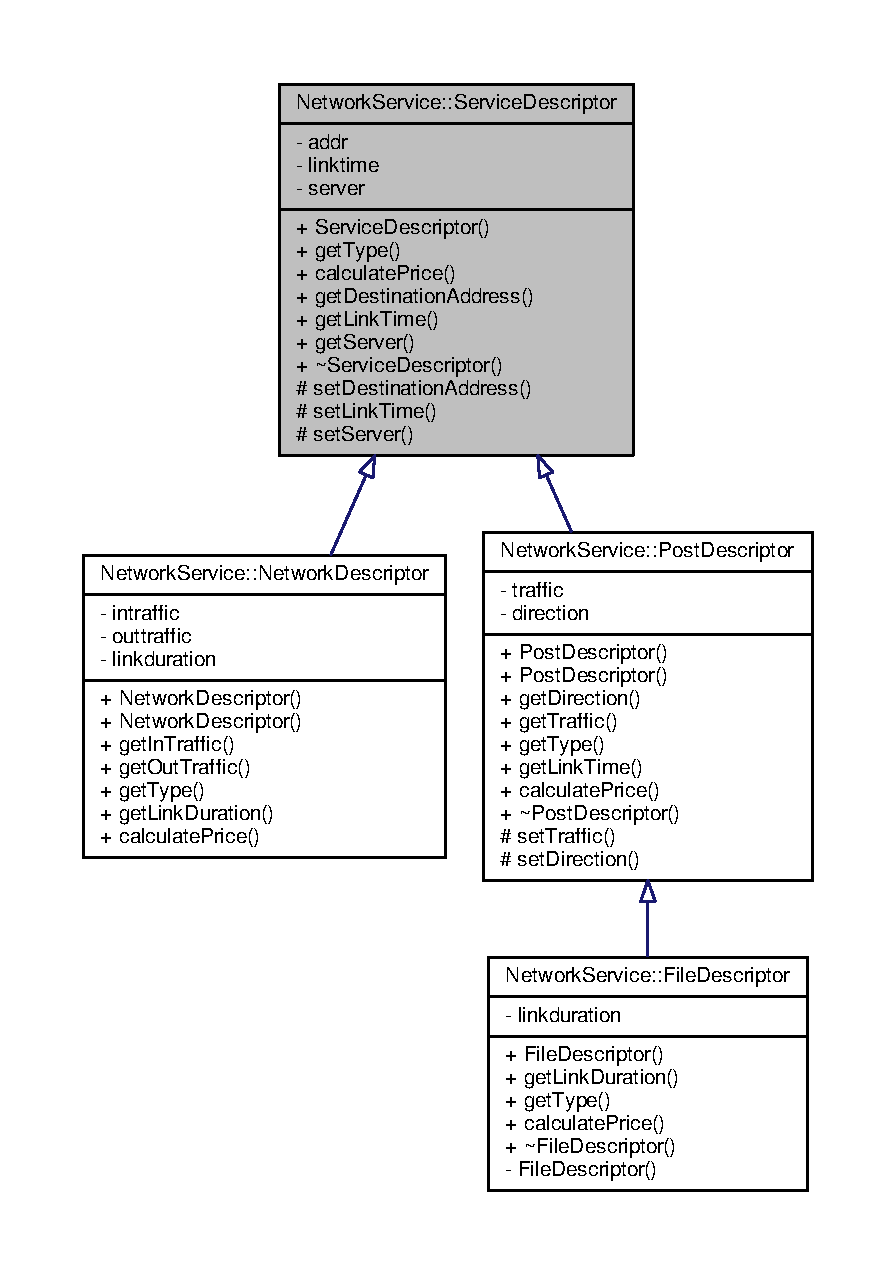
\includegraphics[width=350pt]{class_network_service_1_1_service_descriptor__inherit__graph}
\end{center}
\end{figure}


Граф связей класса Network\+Service\+:\+:Service\+Descriptor\+:
\nopagebreak
\begin{figure}[H]
\begin{center}
\leavevmode
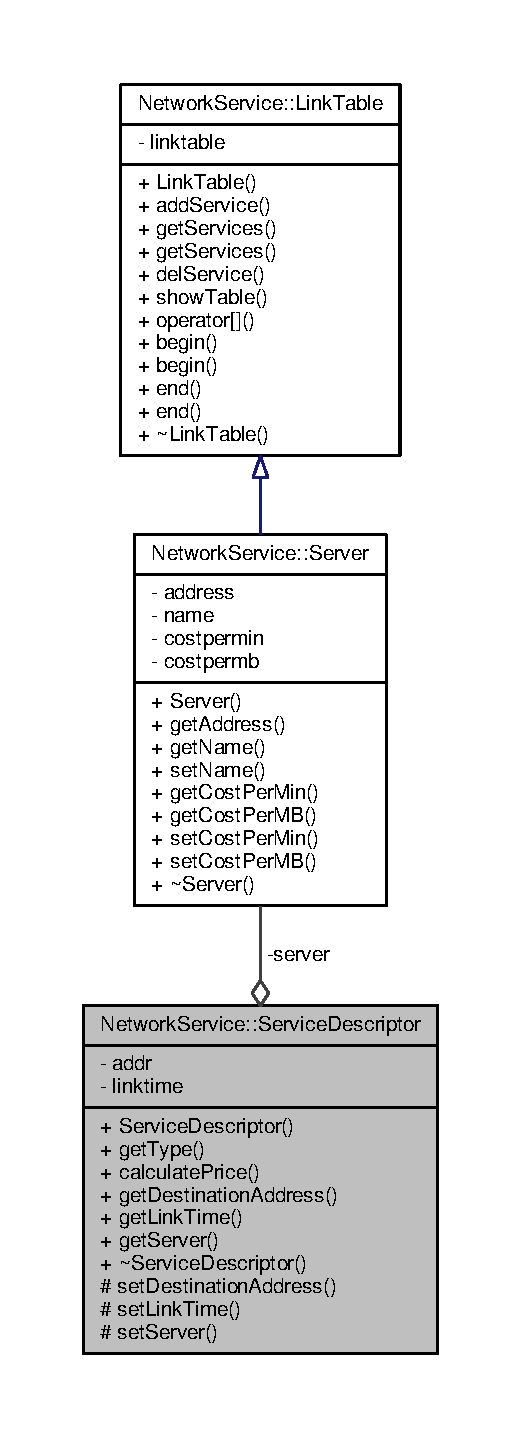
\includegraphics[height=550pt]{class_network_service_1_1_service_descriptor__coll__graph}
\end{center}
\end{figure}
\subsection*{Открытые члены}
\begin{DoxyCompactItemize}
\item 
\hyperlink{class_network_service_1_1_service_descriptor_a18e78e84c574141558bf4bf4ca2dc8a2}{Service\+Descriptor} ()
\begin{DoxyCompactList}\small\item\em Пустой конструктор \end{DoxyCompactList}\item 
virtual std\+::string \hyperlink{class_network_service_1_1_service_descriptor_ac09d5d704a67a7ab2df6d925751ee5cc}{get\+Type} () const =0
\begin{DoxyCompactList}\small\item\em Получение название сервиса \end{DoxyCompactList}\item 
virtual ulong \hyperlink{class_network_service_1_1_service_descriptor_aa2da86b27ac53d8acb1eddf3723a1e44}{calculate\+Price} () const =0
\begin{DoxyCompactList}\small\item\em Рассчет стоимости оказанных услуг \end{DoxyCompactList}\item 
ulong \hyperlink{class_network_service_1_1_service_descriptor_a3717f7dc804127c03d19592e26d7cb9c}{get\+Destination\+Address} () const 
\begin{DoxyCompactList}\small\item\em Получение адреса назначения \end{DoxyCompactList}\item 
const \hyperlink{networkservice_8h_ac877dfabb0f4f6a8184aa821b447e81d}{ftimepoint} \& \hyperlink{class_network_service_1_1_service_descriptor_a0b854ff7100ce01e7f34ca19299bea35}{get\+Link\+Time} () const 
\begin{DoxyCompactList}\small\item\em Получение времени оказания услуги \end{DoxyCompactList}\item 
const \hyperlink{class_network_service_1_1_server}{Server} $\ast$ \hyperlink{class_network_service_1_1_service_descriptor_aeea7b729a1d6dd25fa3fdedd59d3a050}{get\+Server} () const 
\begin{DoxyCompactList}\small\item\em Получение ассоциированного сервера \end{DoxyCompactList}\item 
virtual \hyperlink{class_network_service_1_1_service_descriptor_afc486ca8470d1722103e196284e5f77b}{$\sim$\+Service\+Descriptor} ()
\end{DoxyCompactItemize}
\subsection*{Защищенные члены}
\begin{DoxyCompactItemize}
\item 
void \hyperlink{class_network_service_1_1_service_descriptor_ade61e982c82d03b92f5e096475720bd9}{set\+Destination\+Address} (ulong \hyperlink{class_network_service_1_1_service_descriptor_a0ee74116510749afe1c60a7634d3eae7}{addr})
\begin{DoxyCompactList}\small\item\em Установка адреса назначения \end{DoxyCompactList}\item 
void \hyperlink{class_network_service_1_1_service_descriptor_a7a539e5075ea95a40ec20ebc676093ea}{set\+Link\+Time} (\hyperlink{networkservice_8h_ac877dfabb0f4f6a8184aa821b447e81d}{ftimepoint} \&time)
\begin{DoxyCompactList}\small\item\em Установка времени связи \end{DoxyCompactList}\item 
void \hyperlink{class_network_service_1_1_service_descriptor_a16fa0f2b34adc7665ed32d139d580eb3}{set\+Server} (\hyperlink{class_network_service_1_1_server}{Server} $\ast$srv)
\begin{DoxyCompactList}\small\item\em Установка ассоциированного сервера \end{DoxyCompactList}\end{DoxyCompactItemize}
\subsection*{Закрытые данные}
\begin{DoxyCompactItemize}
\item 
ulong \hyperlink{class_network_service_1_1_service_descriptor_a0ee74116510749afe1c60a7634d3eae7}{addr}
\begin{DoxyCompactList}\small\item\em Адрес назначения \end{DoxyCompactList}\item 
\hyperlink{networkservice_8h_ac877dfabb0f4f6a8184aa821b447e81d}{ftimepoint} \hyperlink{class_network_service_1_1_service_descriptor_a08bfd17afce0cba1954d30bd76a14df4}{linktime}
\begin{DoxyCompactList}\small\item\em Время связи \end{DoxyCompactList}\item 
\hyperlink{class_network_service_1_1_server}{Server} $\ast$ \hyperlink{class_network_service_1_1_service_descriptor_ad504b32ced44a75e0e02ea961d9434c4}{server}
\begin{DoxyCompactList}\small\item\em Указатель на ассоциированный сервер, нужен для рассчета стоимости \end{DoxyCompactList}\end{DoxyCompactItemize}


\subsection{Подробное описание}
Описатель сервиса, абстрактный класс 

Описатели сервисов наследуются от данного класса. Наследуемые классы должны реализовывать методы \hyperlink{class_network_service_1_1_service_descriptor_ac09d5d704a67a7ab2df6d925751ee5cc}{get\+Type()} и \hyperlink{class_network_service_1_1_service_descriptor_aa2da86b27ac53d8acb1eddf3723a1e44}{calculate\+Price()} 

\subsection{Конструктор(ы)}
\hypertarget{class_network_service_1_1_service_descriptor_a18e78e84c574141558bf4bf4ca2dc8a2}{}\index{Network\+Service\+::\+Service\+Descriptor@{Network\+Service\+::\+Service\+Descriptor}!Service\+Descriptor@{Service\+Descriptor}}
\index{Service\+Descriptor@{Service\+Descriptor}!Network\+Service\+::\+Service\+Descriptor@{Network\+Service\+::\+Service\+Descriptor}}
\subsubsection[{Service\+Descriptor}]{\setlength{\rightskip}{0pt plus 5cm}Service\+Descriptor\+::\+Service\+Descriptor (
\begin{DoxyParamCaption}
{}
\end{DoxyParamCaption}
)}\label{class_network_service_1_1_service_descriptor_a18e78e84c574141558bf4bf4ca2dc8a2}


Пустой конструктор 

\hypertarget{class_network_service_1_1_service_descriptor_afc486ca8470d1722103e196284e5f77b}{}\index{Network\+Service\+::\+Service\+Descriptor@{Network\+Service\+::\+Service\+Descriptor}!````~Service\+Descriptor@{$\sim$\+Service\+Descriptor}}
\index{````~Service\+Descriptor@{$\sim$\+Service\+Descriptor}!Network\+Service\+::\+Service\+Descriptor@{Network\+Service\+::\+Service\+Descriptor}}
\subsubsection[{$\sim$\+Service\+Descriptor}]{\setlength{\rightskip}{0pt plus 5cm}Service\+Descriptor\+::$\sim$\+Service\+Descriptor (
\begin{DoxyParamCaption}
{}
\end{DoxyParamCaption}
)\hspace{0.3cm}{\ttfamily [virtual]}}\label{class_network_service_1_1_service_descriptor_afc486ca8470d1722103e196284e5f77b}


\subsection{Методы}
\hypertarget{class_network_service_1_1_service_descriptor_aa2da86b27ac53d8acb1eddf3723a1e44}{}\index{Network\+Service\+::\+Service\+Descriptor@{Network\+Service\+::\+Service\+Descriptor}!calculate\+Price@{calculate\+Price}}
\index{calculate\+Price@{calculate\+Price}!Network\+Service\+::\+Service\+Descriptor@{Network\+Service\+::\+Service\+Descriptor}}
\subsubsection[{calculate\+Price}]{\setlength{\rightskip}{0pt plus 5cm}virtual ulong Network\+Service\+::\+Service\+Descriptor\+::calculate\+Price (
\begin{DoxyParamCaption}
{}
\end{DoxyParamCaption}
) const\hspace{0.3cm}{\ttfamily [pure virtual]}}\label{class_network_service_1_1_service_descriptor_aa2da86b27ac53d8acb1eddf3723a1e44}


Рассчет стоимости оказанных услуг 

\begin{DoxyReturn}{Возвращает}
стоимость оказанных услуг 
\end{DoxyReturn}


Замещается в \hyperlink{class_network_service_1_1_network_descriptor_a515f9b5e56c7027101fcb000e9be96a2}{Network\+Service\+::\+Network\+Descriptor}, \hyperlink{class_network_service_1_1_file_descriptor_a2c480da1613f7072d3113082d1f8cc54}{Network\+Service\+::\+File\+Descriptor} и \hyperlink{class_network_service_1_1_post_descriptor_ae88dfdc2d12299b6d3b14786d16e3251}{Network\+Service\+::\+Post\+Descriptor}.

\hypertarget{class_network_service_1_1_service_descriptor_a3717f7dc804127c03d19592e26d7cb9c}{}\index{Network\+Service\+::\+Service\+Descriptor@{Network\+Service\+::\+Service\+Descriptor}!get\+Destination\+Address@{get\+Destination\+Address}}
\index{get\+Destination\+Address@{get\+Destination\+Address}!Network\+Service\+::\+Service\+Descriptor@{Network\+Service\+::\+Service\+Descriptor}}
\subsubsection[{get\+Destination\+Address}]{\setlength{\rightskip}{0pt plus 5cm}ulong Service\+Descriptor\+::get\+Destination\+Address (
\begin{DoxyParamCaption}
{}
\end{DoxyParamCaption}
) const}\label{class_network_service_1_1_service_descriptor_a3717f7dc804127c03d19592e26d7cb9c}


Получение адреса назначения 

\begin{DoxyReturn}{Возвращает}
Адрес назначения 
\end{DoxyReturn}
\hypertarget{class_network_service_1_1_service_descriptor_a0b854ff7100ce01e7f34ca19299bea35}{}\index{Network\+Service\+::\+Service\+Descriptor@{Network\+Service\+::\+Service\+Descriptor}!get\+Link\+Time@{get\+Link\+Time}}
\index{get\+Link\+Time@{get\+Link\+Time}!Network\+Service\+::\+Service\+Descriptor@{Network\+Service\+::\+Service\+Descriptor}}
\subsubsection[{get\+Link\+Time}]{\setlength{\rightskip}{0pt plus 5cm}const {\bf ftimepoint} \& Service\+Descriptor\+::get\+Link\+Time (
\begin{DoxyParamCaption}
{}
\end{DoxyParamCaption}
) const}\label{class_network_service_1_1_service_descriptor_a0b854ff7100ce01e7f34ca19299bea35}


Получение времени оказания услуги 

\begin{DoxyReturn}{Возвращает}
Ссылка на объект ftimepoint 
\end{DoxyReturn}
\hypertarget{class_network_service_1_1_service_descriptor_aeea7b729a1d6dd25fa3fdedd59d3a050}{}\index{Network\+Service\+::\+Service\+Descriptor@{Network\+Service\+::\+Service\+Descriptor}!get\+Server@{get\+Server}}
\index{get\+Server@{get\+Server}!Network\+Service\+::\+Service\+Descriptor@{Network\+Service\+::\+Service\+Descriptor}}
\subsubsection[{get\+Server}]{\setlength{\rightskip}{0pt plus 5cm}const {\bf Server} $\ast$ Service\+Descriptor\+::get\+Server (
\begin{DoxyParamCaption}
{}
\end{DoxyParamCaption}
) const}\label{class_network_service_1_1_service_descriptor_aeea7b729a1d6dd25fa3fdedd59d3a050}


Получение ассоциированного сервера 

\begin{DoxyReturn}{Возвращает}
Указатель на ассоциированный сервер 
\end{DoxyReturn}
\hypertarget{class_network_service_1_1_service_descriptor_ac09d5d704a67a7ab2df6d925751ee5cc}{}\index{Network\+Service\+::\+Service\+Descriptor@{Network\+Service\+::\+Service\+Descriptor}!get\+Type@{get\+Type}}
\index{get\+Type@{get\+Type}!Network\+Service\+::\+Service\+Descriptor@{Network\+Service\+::\+Service\+Descriptor}}
\subsubsection[{get\+Type}]{\setlength{\rightskip}{0pt plus 5cm}virtual std\+::string Network\+Service\+::\+Service\+Descriptor\+::get\+Type (
\begin{DoxyParamCaption}
{}
\end{DoxyParamCaption}
) const\hspace{0.3cm}{\ttfamily [pure virtual]}}\label{class_network_service_1_1_service_descriptor_ac09d5d704a67a7ab2df6d925751ee5cc}


Получение название сервиса 

\begin{DoxyReturn}{Возвращает}
Строка с названием 
\end{DoxyReturn}


Замещается в \hyperlink{class_network_service_1_1_file_descriptor_a68270f753630bf3ac34c621a56e4f6f7}{Network\+Service\+::\+File\+Descriptor}, \hyperlink{class_network_service_1_1_network_descriptor_abef35df6ca05d7b0ed9e3c0385b9a02a}{Network\+Service\+::\+Network\+Descriptor} и \hyperlink{class_network_service_1_1_post_descriptor_a91b6330d604d4866c85c32187f131431}{Network\+Service\+::\+Post\+Descriptor}.

\hypertarget{class_network_service_1_1_service_descriptor_ade61e982c82d03b92f5e096475720bd9}{}\index{Network\+Service\+::\+Service\+Descriptor@{Network\+Service\+::\+Service\+Descriptor}!set\+Destination\+Address@{set\+Destination\+Address}}
\index{set\+Destination\+Address@{set\+Destination\+Address}!Network\+Service\+::\+Service\+Descriptor@{Network\+Service\+::\+Service\+Descriptor}}
\subsubsection[{set\+Destination\+Address}]{\setlength{\rightskip}{0pt plus 5cm}void Service\+Descriptor\+::set\+Destination\+Address (
\begin{DoxyParamCaption}
\item[{ulong}]{addr}
\end{DoxyParamCaption}
)\hspace{0.3cm}{\ttfamily [protected]}}\label{class_network_service_1_1_service_descriptor_ade61e982c82d03b92f5e096475720bd9}


Установка адреса назначения 


\begin{DoxyParams}{Аргументы}
{\em addr} & Новый адрес назначения \\
\hline
\end{DoxyParams}

\begin{DoxyExceptions}{Исключения}
{\em invalid\+\_\+argument} & Если I\+P адрес не верный \\
\hline
\end{DoxyExceptions}
\hypertarget{class_network_service_1_1_service_descriptor_a7a539e5075ea95a40ec20ebc676093ea}{}\index{Network\+Service\+::\+Service\+Descriptor@{Network\+Service\+::\+Service\+Descriptor}!set\+Link\+Time@{set\+Link\+Time}}
\index{set\+Link\+Time@{set\+Link\+Time}!Network\+Service\+::\+Service\+Descriptor@{Network\+Service\+::\+Service\+Descriptor}}
\subsubsection[{set\+Link\+Time}]{\setlength{\rightskip}{0pt plus 5cm}void Service\+Descriptor\+::set\+Link\+Time (
\begin{DoxyParamCaption}
\item[{{\bf ftimepoint} \&}]{time}
\end{DoxyParamCaption}
)\hspace{0.3cm}{\ttfamily [protected]}}\label{class_network_service_1_1_service_descriptor_a7a539e5075ea95a40ec20ebc676093ea}


Установка времени связи 


\begin{DoxyParams}{Аргументы}
{\em time} & Время связи \\
\hline
\end{DoxyParams}
\hypertarget{class_network_service_1_1_service_descriptor_a16fa0f2b34adc7665ed32d139d580eb3}{}\index{Network\+Service\+::\+Service\+Descriptor@{Network\+Service\+::\+Service\+Descriptor}!set\+Server@{set\+Server}}
\index{set\+Server@{set\+Server}!Network\+Service\+::\+Service\+Descriptor@{Network\+Service\+::\+Service\+Descriptor}}
\subsubsection[{set\+Server}]{\setlength{\rightskip}{0pt plus 5cm}void Service\+Descriptor\+::set\+Server (
\begin{DoxyParamCaption}
\item[{{\bf Server} $\ast$}]{srv}
\end{DoxyParamCaption}
)\hspace{0.3cm}{\ttfamily [protected]}}\label{class_network_service_1_1_service_descriptor_a16fa0f2b34adc7665ed32d139d580eb3}


Установка ассоциированного сервера 


\begin{DoxyParams}{Аргументы}
{\em srv} & Указатель на сервер \\
\hline
\end{DoxyParams}

\begin{DoxyExceptions}{Исключения}
{\em invalid\+\_\+argument} & Если передан nullptr \\
\hline
\end{DoxyExceptions}


\subsection{Данные класса}
\hypertarget{class_network_service_1_1_service_descriptor_a0ee74116510749afe1c60a7634d3eae7}{}\index{Network\+Service\+::\+Service\+Descriptor@{Network\+Service\+::\+Service\+Descriptor}!addr@{addr}}
\index{addr@{addr}!Network\+Service\+::\+Service\+Descriptor@{Network\+Service\+::\+Service\+Descriptor}}
\subsubsection[{addr}]{\setlength{\rightskip}{0pt plus 5cm}ulong Network\+Service\+::\+Service\+Descriptor\+::addr\hspace{0.3cm}{\ttfamily [private]}}\label{class_network_service_1_1_service_descriptor_a0ee74116510749afe1c60a7634d3eae7}


Адрес назначения 

\hypertarget{class_network_service_1_1_service_descriptor_a08bfd17afce0cba1954d30bd76a14df4}{}\index{Network\+Service\+::\+Service\+Descriptor@{Network\+Service\+::\+Service\+Descriptor}!linktime@{linktime}}
\index{linktime@{linktime}!Network\+Service\+::\+Service\+Descriptor@{Network\+Service\+::\+Service\+Descriptor}}
\subsubsection[{linktime}]{\setlength{\rightskip}{0pt plus 5cm}{\bf ftimepoint} Network\+Service\+::\+Service\+Descriptor\+::linktime\hspace{0.3cm}{\ttfamily [private]}}\label{class_network_service_1_1_service_descriptor_a08bfd17afce0cba1954d30bd76a14df4}


Время связи 

\hypertarget{class_network_service_1_1_service_descriptor_ad504b32ced44a75e0e02ea961d9434c4}{}\index{Network\+Service\+::\+Service\+Descriptor@{Network\+Service\+::\+Service\+Descriptor}!server@{server}}
\index{server@{server}!Network\+Service\+::\+Service\+Descriptor@{Network\+Service\+::\+Service\+Descriptor}}
\subsubsection[{server}]{\setlength{\rightskip}{0pt plus 5cm}{\bf Server}$\ast$ Network\+Service\+::\+Service\+Descriptor\+::server\hspace{0.3cm}{\ttfamily [private]}}\label{class_network_service_1_1_service_descriptor_ad504b32ced44a75e0e02ea961d9434c4}


Указатель на ассоциированный сервер, нужен для рассчета стоимости 



Объявления и описания членов классов находятся в файлах\+:\begin{DoxyCompactItemize}
\item 
Network\+Service\+Lib/\hyperlink{servicedescriptor_8h}{servicedescriptor.\+h}\item 
Network\+Service\+Lib/\hyperlink{servicedescriptor_8cpp}{servicedescriptor.\+cpp}\end{DoxyCompactItemize}

\chapter{Файлы}
\hypertarget{application_8cpp}{}\section{Файл Network\+Service\+Lib/application.cpp}
\label{application_8cpp}\index{Network\+Service\+Lib/application.\+cpp@{Network\+Service\+Lib/application.\+cpp}}


Файл, содержащий реализацию класса Application.  


{\ttfamily \#include \char`\"{}networkservice.\+h\char`\"{}}\\*
Граф включаемых заголовочных файлов для application.\+cpp\+:\nopagebreak
\begin{figure}[H]
\begin{center}
\leavevmode
\includegraphics[width=350pt]{application_8cpp__incl}
\end{center}
\end{figure}


\subsection{Подробное описание}
Файл, содержащий реализацию класса Application. 


\hypertarget{application_8h}{}\section{Файл Network\+Service\+Lib/application.h}
\label{application_8h}\index{Network\+Service\+Lib/application.\+h@{Network\+Service\+Lib/application.\+h}}


Файл, содержащий объявление класса Application.  


Граф файлов, в которые включается этот файл\+:\nopagebreak
\begin{figure}[H]
\begin{center}
\leavevmode
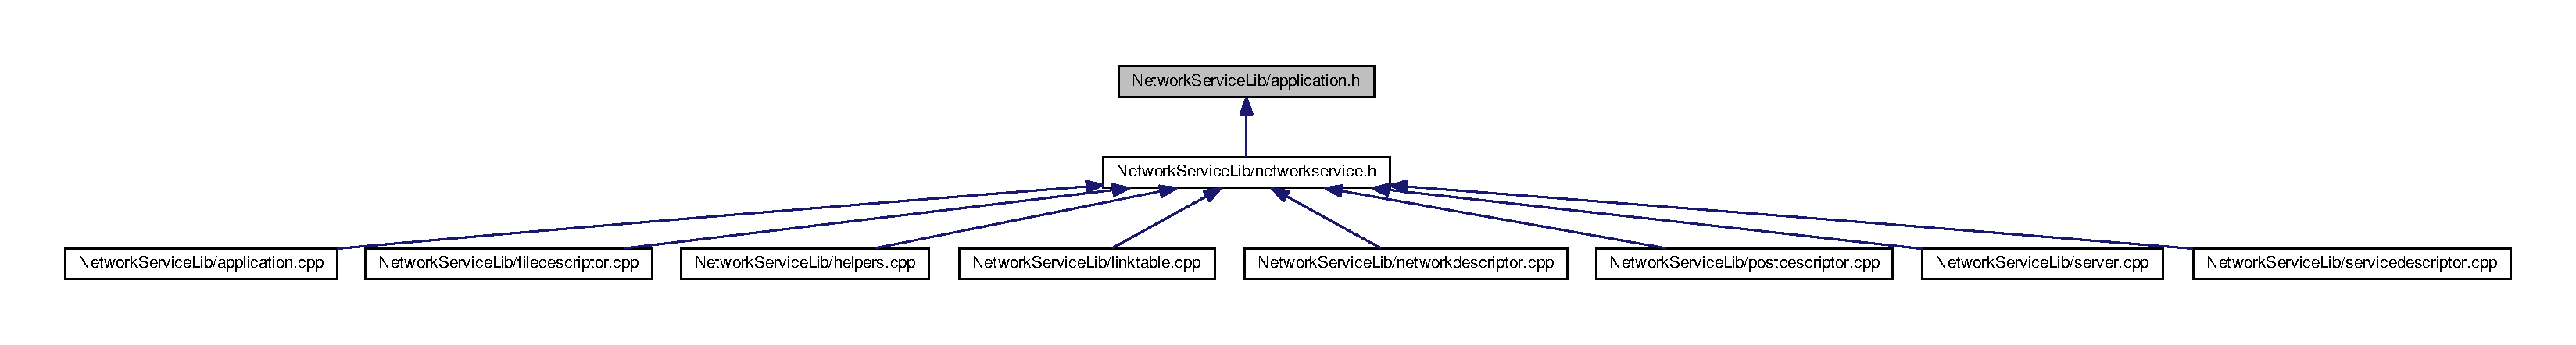
\includegraphics[width=350pt]{application_8h__dep__incl}
\end{center}
\end{figure}
\subsection*{Классы}
\begin{DoxyCompactItemize}
\item 
class \hyperlink{class_network_service_1_1_application}{Network\+Service\+::\+Application}
\begin{DoxyCompactList}\small\item\em Класс, реализующий работу приложения \end{DoxyCompactList}\end{DoxyCompactItemize}
\subsection*{Пространства имен}
\begin{DoxyCompactItemize}
\item 
 \hyperlink{namespace_network_service}{Network\+Service}
\end{DoxyCompactItemize}


\subsection{Подробное описание}
Файл, содержащий объявление класса Application. 


\hypertarget{filedescriptor_8cpp}{}\section{Файл Network\+Service\+Lib/filedescriptor.cpp}
\label{filedescriptor_8cpp}\index{Network\+Service\+Lib/filedescriptor.\+cpp@{Network\+Service\+Lib/filedescriptor.\+cpp}}


Файл, содержащий реализацию класса File\+Descriptor.  


{\ttfamily \#include \char`\"{}networkservice.\+h\char`\"{}}\\*
Граф включаемых заголовочных файлов для filedescriptor.\+cpp\+:\nopagebreak
\begin{figure}[H]
\begin{center}
\leavevmode
\includegraphics[width=350pt]{filedescriptor_8cpp__incl}
\end{center}
\end{figure}


\subsection{Подробное описание}
Файл, содержащий реализацию класса File\+Descriptor. 


\hypertarget{filedescriptor_8h}{}\section{Файл Network\+Service\+Lib/filedescriptor.h}
\label{filedescriptor_8h}\index{Network\+Service\+Lib/filedescriptor.\+h@{Network\+Service\+Lib/filedescriptor.\+h}}


Файл, содержащий объявление класса File\+Descriptor.  


Граф файлов, в которые включается этот файл\+:\nopagebreak
\begin{figure}[H]
\begin{center}
\leavevmode
\includegraphics[width=350pt]{filedescriptor_8h__dep__incl}
\end{center}
\end{figure}
\subsection*{Классы}
\begin{DoxyCompactItemize}
\item 
class \hyperlink{class_network_service_1_1_file_descriptor}{Network\+Service\+::\+File\+Descriptor}
\begin{DoxyCompactList}\small\item\em Класс, описывающий сервис \char`\"{}файл\char`\"{}. \end{DoxyCompactList}\end{DoxyCompactItemize}
\subsection*{Пространства имен}
\begin{DoxyCompactItemize}
\item 
 \hyperlink{namespace_network_service}{Network\+Service}
\end{DoxyCompactItemize}


\subsection{Подробное описание}
Файл, содержащий объявление класса File\+Descriptor. 


\hypertarget{helpers_8cpp}{}\section{Файл Network\+Service\+Lib/helpers.cpp}
\label{helpers_8cpp}\index{Network\+Service\+Lib/helpers.\+cpp@{Network\+Service\+Lib/helpers.\+cpp}}


Файл, содержащий реализацию функций-\/помощников, не принадлежащих какому-\/либо объекту  


{\ttfamily \#include \char`\"{}networkservice.\+h\char`\"{}}\\*
Граф включаемых заголовочных файлов для helpers.\+cpp\+:\nopagebreak
\begin{figure}[H]
\begin{center}
\leavevmode
\includegraphics[width=350pt]{helpers_8cpp__incl}
\end{center}
\end{figure}


\subsection{Подробное описание}
Файл, содержащий реализацию функций-\/помощников, не принадлежащих какому-\/либо объекту 


\hypertarget{helpers_8h}{}\section{Файл Network\+Service\+Lib/helpers.h}
\label{helpers_8h}\index{Network\+Service\+Lib/helpers.\+h@{Network\+Service\+Lib/helpers.\+h}}


Файл, содержащий объявление функций-\/помощников, не принадлежащих какому-\/либо объекту  


Граф файлов, в которые включается этот файл\+:\nopagebreak
\begin{figure}[H]
\begin{center}
\leavevmode
\includegraphics[width=350pt]{helpers_8h__dep__incl}
\end{center}
\end{figure}
\subsection*{Пространства имен}
\begin{DoxyCompactItemize}
\item 
 \hyperlink{namespace_network_service}{Network\+Service}
\end{DoxyCompactItemize}
\subsection*{Функции}
\begin{DoxyCompactItemize}
\item 
std\+::string \hyperlink{namespace_network_service_a814602dad243fba31a6b60d5c56587ac}{Network\+Service\+::\+Long\+I\+Pto\+String} (ulong)
\begin{DoxyCompactList}\small\item\em Преобразование I\+P адреса из ulong-\/представления в строковое \end{DoxyCompactList}\item 
ulong \hyperlink{namespace_network_service_a72263b9e1be1b1629b46daa243761ab9}{Network\+Service\+::string\+To\+Long\+I\+P} (std\+::string)
\begin{DoxyCompactList}\small\item\em Преобразование I\+P адреса из строкового представления в ulong-\/представление \end{DoxyCompactList}\item 
bool \hyperlink{namespace_network_service_a4e78f6978578fd3ee62f1c3f8b555009}{Network\+Service\+::is\+Valid\+I\+P} (ulong)
\begin{DoxyCompactList}\small\item\em Проверка, является ли I\+P адрес верным \end{DoxyCompactList}\end{DoxyCompactItemize}


\subsection{Подробное описание}
Файл, содержащий объявление функций-\/помощников, не принадлежащих какому-\/либо объекту 


\hypertarget{linktable_8cpp}{}\section{Файл Network\+Service\+Lib/linktable.cpp}
\label{linktable_8cpp}\index{Network\+Service\+Lib/linktable.\+cpp@{Network\+Service\+Lib/linktable.\+cpp}}


Файл, содержащий реализацию класса Link\+Table.  


{\ttfamily \#include \char`\"{}networkservice.\+h\char`\"{}}\\*
Граф включаемых заголовочных файлов для linktable.\+cpp\+:\nopagebreak
\begin{figure}[H]
\begin{center}
\leavevmode
\includegraphics[width=350pt]{linktable_8cpp__incl}
\end{center}
\end{figure}


\subsection{Подробное описание}
Файл, содержащий реализацию класса Link\+Table. 


\hypertarget{linktable_8h}{}\section{Файл Network\+Service\+Lib/linktable.h}
\label{linktable_8h}\index{Network\+Service\+Lib/linktable.\+h@{Network\+Service\+Lib/linktable.\+h}}


Файл, содержащий объявление класса Link\+Table.  


Граф файлов, в которые включается этот файл\+:\nopagebreak
\begin{figure}[H]
\begin{center}
\leavevmode
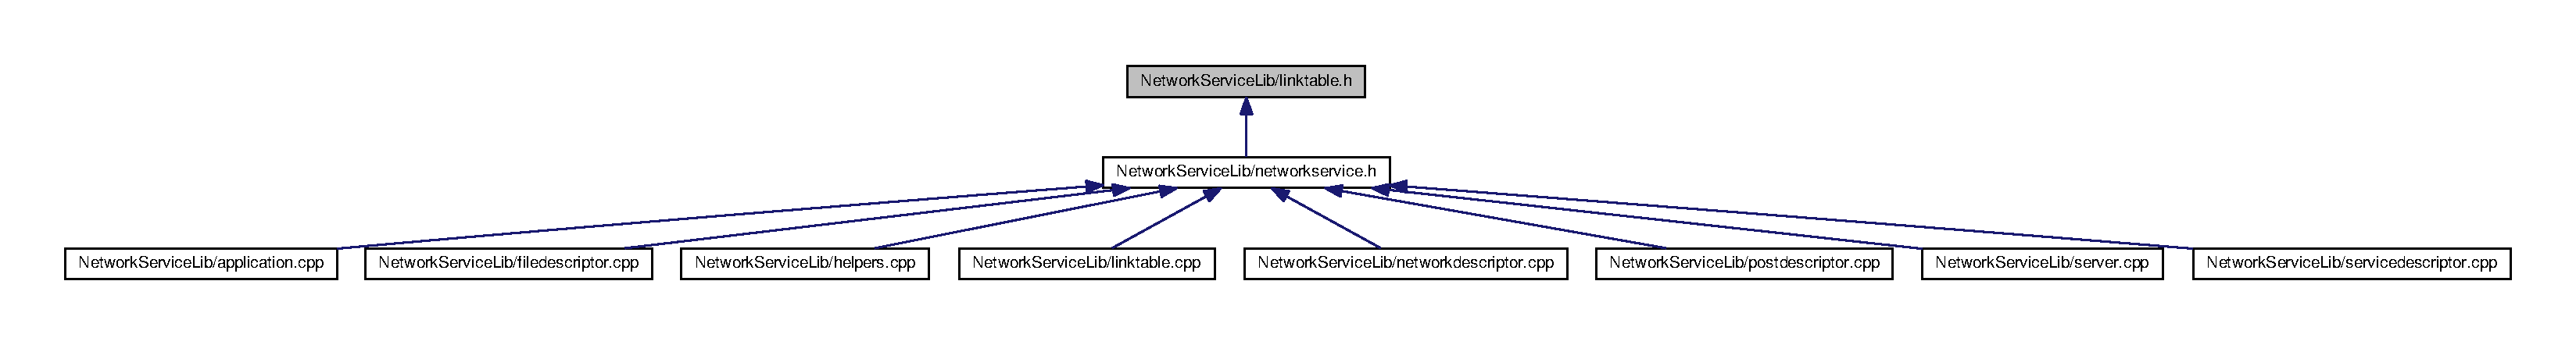
\includegraphics[width=350pt]{linktable_8h__dep__incl}
\end{center}
\end{figure}
\subsection*{Классы}
\begin{DoxyCompactItemize}
\item 
class \hyperlink{class_network_service_1_1_link_table}{Network\+Service\+::\+Link\+Table}
\begin{DoxyCompactList}\small\item\em Класс, реализующий \char`\"{}таблицу связи\char`\"{}. \end{DoxyCompactList}\end{DoxyCompactItemize}
\subsection*{Пространства имен}
\begin{DoxyCompactItemize}
\item 
 \hyperlink{namespace_network_service}{Network\+Service}
\end{DoxyCompactItemize}


\subsection{Подробное описание}
Файл, содержащий объявление класса Link\+Table. 


\hypertarget{myiterator_8h}{}\section{Файл Network\+Service\+Lib/myiterator.h}
\label{myiterator_8h}\index{Network\+Service\+Lib/myiterator.\+h@{Network\+Service\+Lib/myiterator.\+h}}


Файл, содержащий шаблонных классов My\+Iterator, My\+Const\+Iterator.  


Граф файлов, в которые включается этот файл\+:\nopagebreak
\begin{figure}[H]
\begin{center}
\leavevmode
\includegraphics[width=350pt]{myiterator_8h__dep__incl}
\end{center}
\end{figure}
\subsection*{Классы}
\begin{DoxyCompactItemize}
\item 
class \hyperlink{class_network_service_1_1_my_iterator}{Network\+Service\+::\+My\+Iterator$<$ T $>$}
\begin{DoxyCompactList}\small\item\em Шаблонный класс итератора \end{DoxyCompactList}\item 
class \hyperlink{class_network_service_1_1_my_const_iterator}{Network\+Service\+::\+My\+Const\+Iterator$<$ T $>$}
\begin{DoxyCompactList}\small\item\em Шаблонный класс итератора \end{DoxyCompactList}\end{DoxyCompactItemize}
\subsection*{Пространства имен}
\begin{DoxyCompactItemize}
\item 
 \hyperlink{namespace_network_service}{Network\+Service}
\end{DoxyCompactItemize}


\subsection{Подробное описание}
Файл, содержащий шаблонных классов My\+Iterator, My\+Const\+Iterator. 


\hypertarget{networkdescriptor_8cpp}{}\section{Файл Network\+Service\+Lib/networkdescriptor.cpp}
\label{networkdescriptor_8cpp}\index{Network\+Service\+Lib/networkdescriptor.\+cpp@{Network\+Service\+Lib/networkdescriptor.\+cpp}}


Файл, содержащий реализацию класса Network\+Descriptor.  


{\ttfamily \#include \char`\"{}networkservice.\+h\char`\"{}}\\*
Граф включаемых заголовочных файлов для networkdescriptor.\+cpp\+:\nopagebreak
\begin{figure}[H]
\begin{center}
\leavevmode
\includegraphics[width=350pt]{networkdescriptor_8cpp__incl}
\end{center}
\end{figure}


\subsection{Подробное описание}
Файл, содержащий реализацию класса Network\+Descriptor. 


\hypertarget{networkdescriptor_8h}{}\section{Файл Network\+Service\+Lib/networkdescriptor.h}
\label{networkdescriptor_8h}\index{Network\+Service\+Lib/networkdescriptor.\+h@{Network\+Service\+Lib/networkdescriptor.\+h}}


Файл, содержащий объявление класса Network\+Descriptor.  


Граф файлов, в которые включается этот файл\+:\nopagebreak
\begin{figure}[H]
\begin{center}
\leavevmode
\includegraphics[width=350pt]{networkdescriptor_8h__dep__incl}
\end{center}
\end{figure}
\subsection*{Классы}
\begin{DoxyCompactItemize}
\item 
class \hyperlink{class_network_service_1_1_network_descriptor}{Network\+Service\+::\+Network\+Descriptor}
\begin{DoxyCompactList}\small\item\em Описатель сервиса \char`\"{}сеть\char`\"{}, наследуется от \hyperlink{class_network_service_1_1_service_descriptor}{Service\+Descriptor}. \end{DoxyCompactList}\end{DoxyCompactItemize}
\subsection*{Пространства имен}
\begin{DoxyCompactItemize}
\item 
 \hyperlink{namespace_network_service}{Network\+Service}
\end{DoxyCompactItemize}


\subsection{Подробное описание}
Файл, содержащий объявление класса Network\+Descriptor. 


\hypertarget{networkservice_8h}{}\section{Файл Network\+Service\+Lib/networkservice.h}
\label{networkservice_8h}\index{Network\+Service\+Lib/networkservice.\+h@{Network\+Service\+Lib/networkservice.\+h}}


Файл, содержаший все необходимые определения и включения для работы библиотеки  


{\ttfamily \#include $<$chrono$>$}\\*
{\ttfamily \#include $<$string$>$}\\*
{\ttfamily \#include $<$vector$>$}\\*
{\ttfamily \#include $<$utility$>$}\\*
{\ttfamily \#include $<$sys/socket.\+h$>$}\\*
{\ttfamily \#include $<$netinet/in.\+h$>$}\\*
{\ttfamily \#include $<$arpa/inet.\+h$>$}\\*
{\ttfamily \#include $<$stdexcept$>$}\\*
{\ttfamily \#include $<$algorithm$>$}\\*
{\ttfamily \#include $<$typeinfo$>$}\\*
{\ttfamily \#include $<$rapidjson/document.\+h$>$}\\*
{\ttfamily \#include $<$rapidjson/writer.\+h$>$}\\*
{\ttfamily \#include $<$rapidjson/stringbuffer.\+h$>$}\\*
{\ttfamily \#include $<$fstream$>$}\\*
{\ttfamily \#include \char`\"{}helpers.\+h\char`\"{}}\\*
{\ttfamily \#include \char`\"{}servicedescriptor.\+h\char`\"{}}\\*
{\ttfamily \#include \char`\"{}postdescriptor.\+h\char`\"{}}\\*
{\ttfamily \#include \char`\"{}filedescriptor.\+h\char`\"{}}\\*
{\ttfamily \#include \char`\"{}networkdescriptor.\+h\char`\"{}}\\*
{\ttfamily \#include \char`\"{}myiterator.\+h\char`\"{}}\\*
{\ttfamily \#include \char`\"{}linktable.\+h\char`\"{}}\\*
{\ttfamily \#include \char`\"{}server.\+h\char`\"{}}\\*
{\ttfamily \#include \char`\"{}application.\+h\char`\"{}}\\*
Граф включаемых заголовочных файлов для networkservice.\+h\+:\nopagebreak
\begin{figure}[H]
\begin{center}
\leavevmode
\includegraphics[width=350pt]{networkservice_8h__incl}
\end{center}
\end{figure}
Граф файлов, в которые включается этот файл\+:\nopagebreak
\begin{figure}[H]
\begin{center}
\leavevmode
\includegraphics[width=350pt]{networkservice_8h__dep__incl}
\end{center}
\end{figure}
\subsection*{Пространства имен}
\begin{DoxyCompactItemize}
\item 
 \hyperlink{namespace_network_service}{Network\+Service}
\end{DoxyCompactItemize}
\subsection*{Определения типов}
\begin{DoxyCompactItemize}
\item 
typedef std\+::chrono\+::system\+\_\+clock \hyperlink{networkservice_8h_a97d64aa956870c03861fd53e772217f1}{Time}
\begin{DoxyCompactList}\small\item\em Системные часы \end{DoxyCompactList}\item 
typedef std\+::chrono\+::milliseconds \hyperlink{networkservice_8h_a55ca616433f0dffb4cdc575fb4daafe4}{ms}
\begin{DoxyCompactList}\small\item\em Милисекунда \end{DoxyCompactList}\item 
typedef std\+::chrono\+::time\+\_\+point$<$ \hyperlink{networkservice_8h_a97d64aa956870c03861fd53e772217f1}{Time} $>$ \hyperlink{networkservice_8h_ac877dfabb0f4f6a8184aa821b447e81d}{ftimepoint}
\begin{DoxyCompactList}\small\item\em Специализация time\+\_\+point для системных часов \end{DoxyCompactList}\item 
typedef std\+::chrono\+::duration$<$ float $>$ \hyperlink{networkservice_8h_a476cc728ef971cba9111c75ea41a760a}{fduration}
\begin{DoxyCompactList}\small\item\em Специализация duration для типа float. \end{DoxyCompactList}\end{DoxyCompactItemize}
\subsection*{Перечисления}
\begin{DoxyCompactItemize}
\item 
enum \hyperlink{namespace_network_service_abe1196dad9e8afcbc5c6b38196ce2c65}{Network\+Service\+::\+Direction} \{ \hyperlink{namespace_network_service_abe1196dad9e8afcbc5c6b38196ce2c65aba432dcf573f50b84f5ed73af5d4a1d1}{Network\+Service\+::\+S\+E\+N\+D}, 
\hyperlink{namespace_network_service_abe1196dad9e8afcbc5c6b38196ce2c65ad723a3e2a611f41c5add1e872173dc45}{Network\+Service\+::\+R\+E\+C\+V}
 \}
\begin{DoxyCompactList}\small\item\em Направление передачи данных \end{DoxyCompactList}\end{DoxyCompactItemize}
\subsection*{Переменные}
\begin{DoxyCompactItemize}
\item 
static const ulong \hyperlink{networkservice_8h_a6271778876b139199b3f0f059978a236}{minute\+\_\+k} = std\+::chrono\+::minutes\+::period\+::num / std\+::chrono\+::minutes\+::period\+::den
\begin{DoxyCompactList}\small\item\em Коэфиициент для получения количества минут из объекта duration. \end{DoxyCompactList}\end{DoxyCompactItemize}


\subsection{Подробное описание}
Файл, содержаший все необходимые определения и включения для работы библиотеки 

В приложении используйте его. 

\subsection{Типы}
\hypertarget{networkservice_8h_a476cc728ef971cba9111c75ea41a760a}{}\index{networkservice.\+h@{networkservice.\+h}!fduration@{fduration}}
\index{fduration@{fduration}!networkservice.\+h@{networkservice.\+h}}
\subsubsection[{fduration}]{\setlength{\rightskip}{0pt plus 5cm}typedef std\+::chrono\+::duration$<$float$>$ {\bf fduration}}\label{networkservice_8h_a476cc728ef971cba9111c75ea41a760a}


Специализация duration для типа float. 

\hypertarget{networkservice_8h_ac877dfabb0f4f6a8184aa821b447e81d}{}\index{networkservice.\+h@{networkservice.\+h}!ftimepoint@{ftimepoint}}
\index{ftimepoint@{ftimepoint}!networkservice.\+h@{networkservice.\+h}}
\subsubsection[{ftimepoint}]{\setlength{\rightskip}{0pt plus 5cm}typedef std\+::chrono\+::time\+\_\+point$<${\bf Time}$>$ {\bf ftimepoint}}\label{networkservice_8h_ac877dfabb0f4f6a8184aa821b447e81d}


Специализация time\+\_\+point для системных часов 

\hypertarget{networkservice_8h_a55ca616433f0dffb4cdc575fb4daafe4}{}\index{networkservice.\+h@{networkservice.\+h}!ms@{ms}}
\index{ms@{ms}!networkservice.\+h@{networkservice.\+h}}
\subsubsection[{ms}]{\setlength{\rightskip}{0pt plus 5cm}typedef std\+::chrono\+::milliseconds {\bf ms}}\label{networkservice_8h_a55ca616433f0dffb4cdc575fb4daafe4}


Милисекунда 

\hypertarget{networkservice_8h_a97d64aa956870c03861fd53e772217f1}{}\index{networkservice.\+h@{networkservice.\+h}!Time@{Time}}
\index{Time@{Time}!networkservice.\+h@{networkservice.\+h}}
\subsubsection[{Time}]{\setlength{\rightskip}{0pt plus 5cm}typedef std\+::chrono\+::system\+\_\+clock {\bf Time}}\label{networkservice_8h_a97d64aa956870c03861fd53e772217f1}


Системные часы 



\subsection{Переменные}
\hypertarget{networkservice_8h_a6271778876b139199b3f0f059978a236}{}\index{networkservice.\+h@{networkservice.\+h}!minute\+\_\+k@{minute\+\_\+k}}
\index{minute\+\_\+k@{minute\+\_\+k}!networkservice.\+h@{networkservice.\+h}}
\subsubsection[{minute\+\_\+k}]{\setlength{\rightskip}{0pt plus 5cm}const ulong minute\+\_\+k = std\+::chrono\+::minutes\+::period\+::num / std\+::chrono\+::minutes\+::period\+::den\hspace{0.3cm}{\ttfamily [static]}}\label{networkservice_8h_a6271778876b139199b3f0f059978a236}


Коэфиициент для получения количества минут из объекта duration. 


\hypertarget{networkservicelib_8cpp}{}\section{Файл Network\+Service\+Lib/networkservicelib.cpp}
\label{networkservicelib_8cpp}\index{Network\+Service\+Lib/networkservicelib.\+cpp@{Network\+Service\+Lib/networkservicelib.\+cpp}}

\hypertarget{postdescriptor_8cpp}{}\section{Файл Network\+Service\+Lib/postdescriptor.cpp}
\label{postdescriptor_8cpp}\index{Network\+Service\+Lib/postdescriptor.\+cpp@{Network\+Service\+Lib/postdescriptor.\+cpp}}


Файл, содержащий реализацию класса Post\+Descriptor.  


{\ttfamily \#include \char`\"{}networkservice.\+h\char`\"{}}\\*
Граф включаемых заголовочных файлов для postdescriptor.\+cpp\+:\nopagebreak
\begin{figure}[H]
\begin{center}
\leavevmode
\includegraphics[width=350pt]{postdescriptor_8cpp__incl}
\end{center}
\end{figure}


\subsection{Подробное описание}
Файл, содержащий реализацию класса Post\+Descriptor. 


\hypertarget{postdescriptor_8h}{}\section{Файл Network\+Service\+Lib/postdescriptor.h}
\label{postdescriptor_8h}\index{Network\+Service\+Lib/postdescriptor.\+h@{Network\+Service\+Lib/postdescriptor.\+h}}


Файл, содержащий объявление класса Post\+Descriptor.  


Граф файлов, в которые включается этот файл\+:\nopagebreak
\begin{figure}[H]
\begin{center}
\leavevmode
\includegraphics[width=350pt]{postdescriptor_8h__dep__incl}
\end{center}
\end{figure}
\subsection*{Классы}
\begin{DoxyCompactItemize}
\item 
class \hyperlink{class_network_service_1_1_post_descriptor}{Network\+Service\+::\+Post\+Descriptor}
\begin{DoxyCompactList}\small\item\em Описатель сервиса \char`\"{}почта\char`\"{}, наследуемый от \hyperlink{class_network_service_1_1_service_descriptor}{Service\+Descriptor}. \end{DoxyCompactList}\end{DoxyCompactItemize}
\subsection*{Пространства имен}
\begin{DoxyCompactItemize}
\item 
 \hyperlink{namespace_network_service}{Network\+Service}
\end{DoxyCompactItemize}


\subsection{Подробное описание}
Файл, содержащий объявление класса Post\+Descriptor. 


\hypertarget{server_8cpp}{}\section{Файл Network\+Service\+Lib/server.cpp}
\label{server_8cpp}\index{Network\+Service\+Lib/server.\+cpp@{Network\+Service\+Lib/server.\+cpp}}


Файл, содержащий реализацию класса Server.  


{\ttfamily \#include \char`\"{}networkservice.\+h\char`\"{}}\\*
Граф включаемых заголовочных файлов для server.\+cpp\+:\nopagebreak
\begin{figure}[H]
\begin{center}
\leavevmode
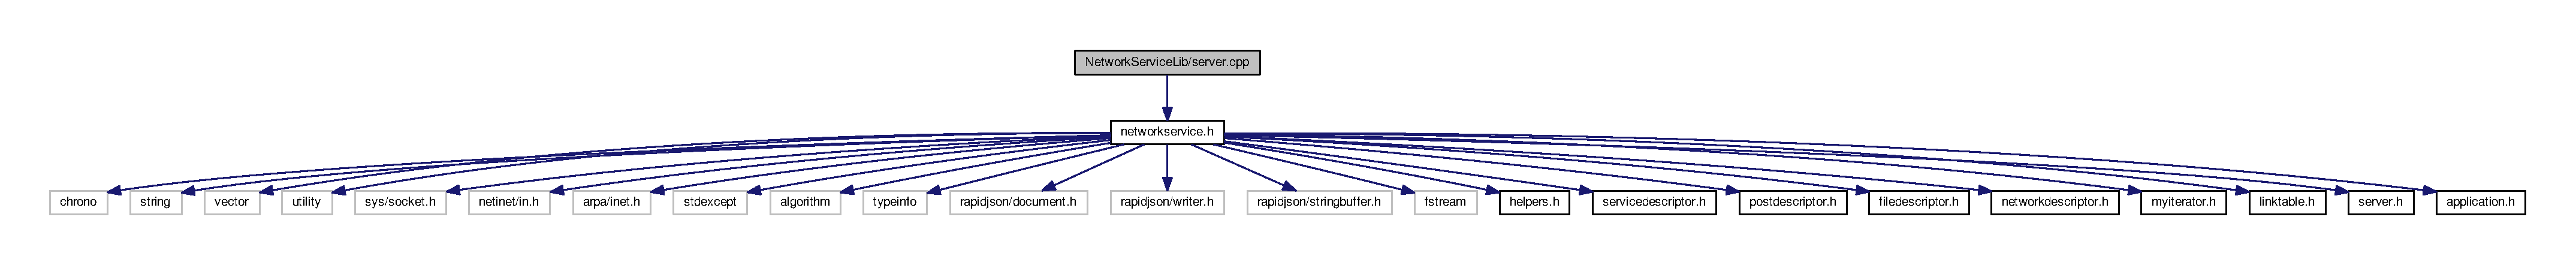
\includegraphics[width=350pt]{server_8cpp__incl}
\end{center}
\end{figure}


\subsection{Подробное описание}
Файл, содержащий реализацию класса Server. 


\hypertarget{server_8h}{}\section{Файл Network\+Service\+Lib/server.h}
\label{server_8h}\index{Network\+Service\+Lib/server.\+h@{Network\+Service\+Lib/server.\+h}}


Файл, содержащий объявление класса Server.  


Граф файлов, в которые включается этот файл\+:\nopagebreak
\begin{figure}[H]
\begin{center}
\leavevmode
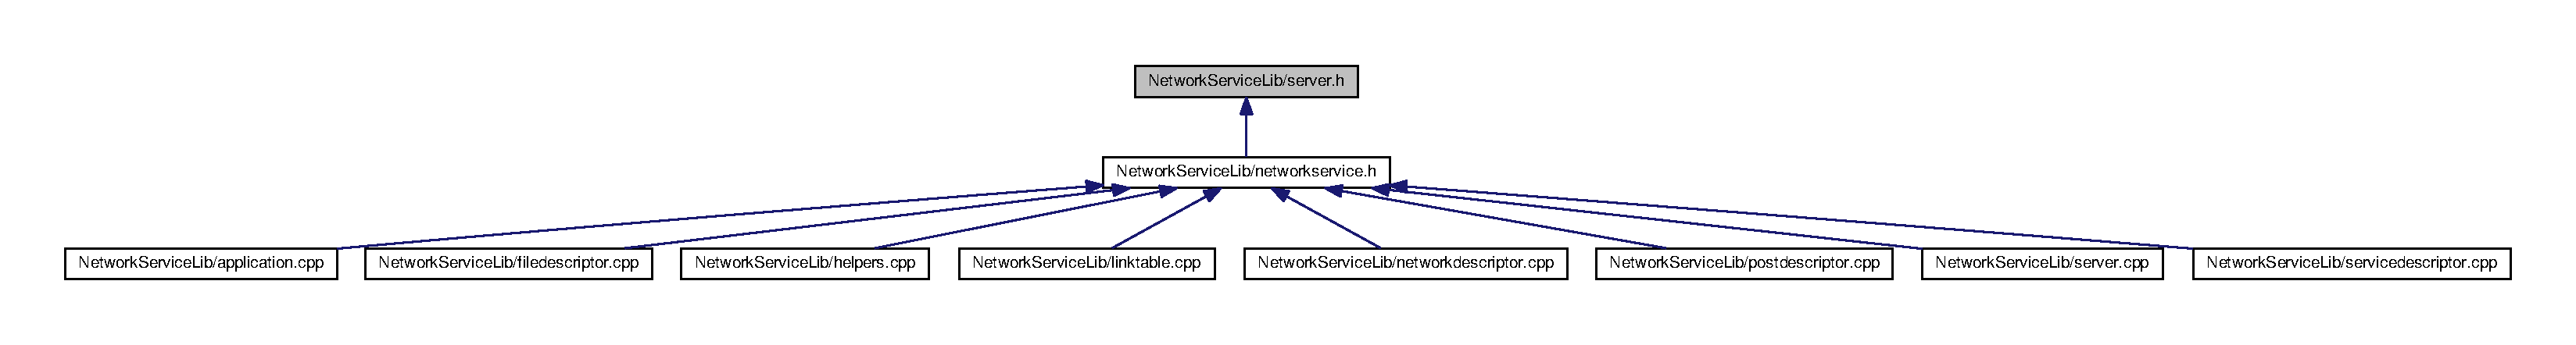
\includegraphics[width=350pt]{server_8h__dep__incl}
\end{center}
\end{figure}
\subsection*{Классы}
\begin{DoxyCompactItemize}
\item 
class \hyperlink{class_network_service_1_1_server}{Network\+Service\+::\+Server}
\begin{DoxyCompactList}\small\item\em Описатель сервера \end{DoxyCompactList}\end{DoxyCompactItemize}
\subsection*{Пространства имен}
\begin{DoxyCompactItemize}
\item 
 \hyperlink{namespace_network_service}{Network\+Service}
\end{DoxyCompactItemize}


\subsection{Подробное описание}
Файл, содержащий объявление класса Server. 


\hypertarget{servicedescriptor_8cpp}{}\section{Файл Network\+Service\+Lib/servicedescriptor.cpp}
\label{servicedescriptor_8cpp}\index{Network\+Service\+Lib/servicedescriptor.\+cpp@{Network\+Service\+Lib/servicedescriptor.\+cpp}}


Файл, содержащий реализацию класса Service\+Descriptor.  


{\ttfamily \#include \char`\"{}networkservice.\+h\char`\"{}}\\*
Граф включаемых заголовочных файлов для servicedescriptor.\+cpp\+:\nopagebreak
\begin{figure}[H]
\begin{center}
\leavevmode
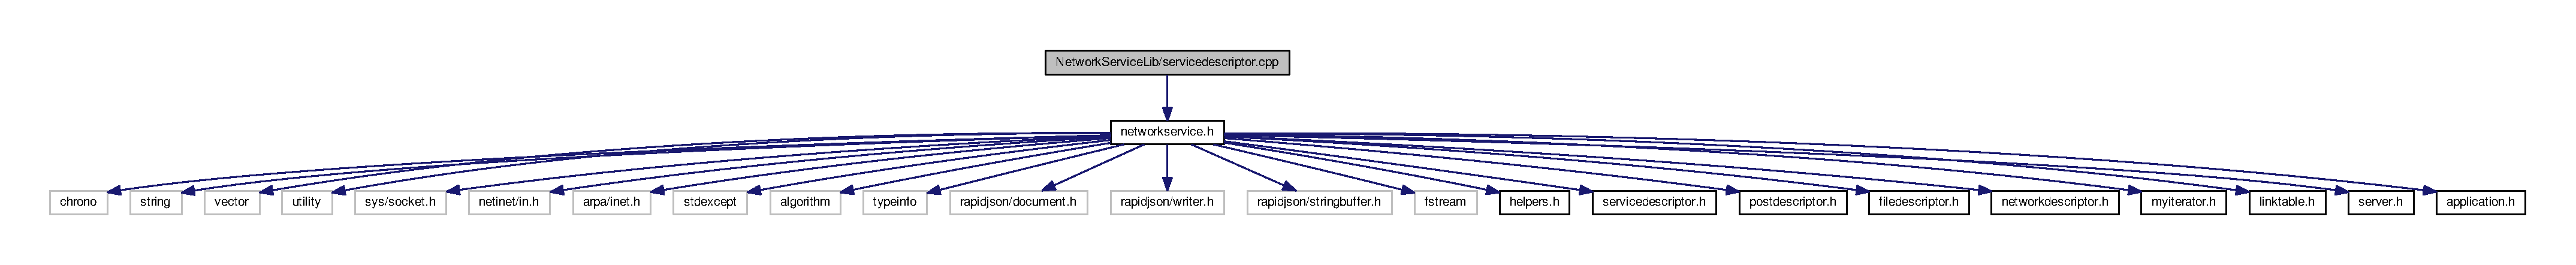
\includegraphics[width=350pt]{servicedescriptor_8cpp__incl}
\end{center}
\end{figure}


\subsection{Подробное описание}
Файл, содержащий реализацию класса Service\+Descriptor. 


\hypertarget{servicedescriptor_8h}{}\section{Файл Network\+Service\+Lib/servicedescriptor.h}
\label{servicedescriptor_8h}\index{Network\+Service\+Lib/servicedescriptor.\+h@{Network\+Service\+Lib/servicedescriptor.\+h}}


Файл, содержащий объявление абстрактного класса Service\+Descriptor.  


Граф файлов, в которые включается этот файл\+:\nopagebreak
\begin{figure}[H]
\begin{center}
\leavevmode
\includegraphics[width=350pt]{servicedescriptor_8h__dep__incl}
\end{center}
\end{figure}
\subsection*{Классы}
\begin{DoxyCompactItemize}
\item 
class \hyperlink{class_network_service_1_1_service_descriptor}{Network\+Service\+::\+Service\+Descriptor}
\begin{DoxyCompactList}\small\item\em Описатель сервиса, абстрактный класс \end{DoxyCompactList}\end{DoxyCompactItemize}
\subsection*{Пространства имен}
\begin{DoxyCompactItemize}
\item 
 \hyperlink{namespace_network_service}{Network\+Service}
\end{DoxyCompactItemize}


\subsection{Подробное описание}
Файл, содержащий объявление абстрактного класса Service\+Descriptor. 


%--- End generated contents ---

% Index
\backmatter
\newpage
\phantomsection
\clearemptydoublepage
\addcontentsline{toc}{chapter}{Алфавитный указатель}
\printindex

\end{document}
